\documentclass[twoside]{book}

% Packages required by doxygen
\usepackage{calc}
\usepackage{doxygen}
\usepackage{graphicx}
\usepackage[utf8]{inputenc}
\usepackage{makeidx}
\usepackage{multicol}
\usepackage{multirow}
\usepackage{textcomp}
\usepackage[table]{xcolor}

% Font selection
\usepackage[T1]{fontenc}
\usepackage{mathptmx}
\usepackage[scaled=.90]{helvet}
\usepackage{courier}
\usepackage{amssymb}
\usepackage{sectsty}
\renewcommand{\familydefault}{\sfdefault}
\allsectionsfont{%
  \fontseries{bc}\selectfont%
  \color{darkgray}%
}
\renewcommand{\DoxyLabelFont}{%
  \fontseries{bc}\selectfont%
  \color{darkgray}%
}

% Page & text layout
\usepackage{geometry}
\geometry{%
  a4paper,%
  top=2.5cm,%
  bottom=2.5cm,%
  left=2.5cm,%
  right=2.5cm%
}
\tolerance=750
\hfuzz=15pt
\hbadness=750
\setlength{\emergencystretch}{15pt}
\setlength{\parindent}{0cm}
\setlength{\parskip}{0.2cm}
\makeatletter
\renewcommand{\paragraph}{%
  \@startsection{paragraph}{4}{0ex}{-1.0ex}{1.0ex}{%
    \normalfont\normalsize\bfseries\SS@parafont%
  }%
}
\renewcommand{\subparagraph}{%
  \@startsection{subparagraph}{5}{0ex}{-1.0ex}{1.0ex}{%
    \normalfont\normalsize\bfseries\SS@subparafont%
  }%
}
\makeatother

% Headers & footers
\usepackage{fancyhdr}
\pagestyle{fancyplain}
\fancyhead[LE]{\fancyplain{}{\bfseries\thepage}}
\fancyhead[CE]{\fancyplain{}{}}
\fancyhead[RE]{\fancyplain{}{\bfseries\leftmark}}
\fancyhead[LO]{\fancyplain{}{\bfseries\rightmark}}
\fancyhead[CO]{\fancyplain{}{}}
\fancyhead[RO]{\fancyplain{}{\bfseries\thepage}}
\fancyfoot[LE]{\fancyplain{}{}}
\fancyfoot[CE]{\fancyplain{}{}}
\fancyfoot[RE]{\fancyplain{}{\bfseries\scriptsize Generated on Mon Dec 23 2013 00\-:20\-:19 for D\-R\-D\-S\-P by Doxygen }}
\fancyfoot[LO]{\fancyplain{}{\bfseries\scriptsize Generated on Mon Dec 23 2013 00\-:20\-:19 for D\-R\-D\-S\-P by Doxygen }}
\fancyfoot[CO]{\fancyplain{}{}}
\fancyfoot[RO]{\fancyplain{}{}}
\renewcommand{\footrulewidth}{0.4pt}
\renewcommand{\chaptermark}[1]{%
  \markboth{#1}{}%
}
\renewcommand{\sectionmark}[1]{%
  \markright{\thesection\ #1}%
}

% Indices & bibliography
\usepackage{natbib}
\usepackage[titles]{tocloft}
\setcounter{tocdepth}{3}
\setcounter{secnumdepth}{5}
\makeindex

% Hyperlinks (required, but should be loaded last)
\usepackage{ifpdf}
\ifpdf
  \usepackage[pdftex,pagebackref=true]{hyperref}
\else
  \usepackage[ps2pdf,pagebackref=true]{hyperref}
\fi
\hypersetup{%
  colorlinks=true,%
  linkcolor=blue,%
  citecolor=blue,%
  unicode%
}

% Custom commands
\newcommand{\clearemptydoublepage}{%
  \newpage{\pagestyle{empty}\cleardoublepage}%
}


%===== C O N T E N T S =====

\begin{document}

% Titlepage & ToC
\hypersetup{pageanchor=false}
\pagenumbering{roman}
\begin{titlepage}
\vspace*{7cm}
\begin{center}%
{\Large D\-R\-D\-S\-P }\\
\vspace*{1cm}
{\large Generated by Doxygen 1.8.5}\\
\vspace*{0.5cm}
{\small Mon Dec 23 2013 00:20:19}\\
\end{center}
\end{titlepage}
\clearemptydoublepage
\tableofcontents
\clearemptydoublepage
\pagenumbering{arabic}
\hypersetup{pageanchor=true}

%--- Begin generated contents ---
\chapter{Hierarchical Index}
\section{Class Hierarchy}
This inheritance list is sorted roughly, but not completely, alphabetically\-:\begin{DoxyCompactList}
\item \contentsline{section}{D\-R\-D\-S\-P\-:\-:A\-A\-B\-B}{\pageref{struct_d_r_d_s_p_1_1_a_a_b_b}}{}
\item \contentsline{section}{D\-R\-D\-S\-P\-:\-:Affine\-Parameter\-Map}{\pageref{struct_d_r_d_s_p_1_1_affine_parameter_map}}{}
\item \contentsline{section}{D\-R\-D\-S\-P\-:\-:Bifurcation\-Diagram$<$ Parameter, Value $>$}{\pageref{struct_d_r_d_s_p_1_1_bifurcation_diagram}}{}
\item \contentsline{section}{D\-R\-D\-S\-P\-:\-:Bifurcation\-Diagram\-Generator$<$ Family, Solver $>$}{\pageref{struct_d_r_d_s_p_1_1_bifurcation_diagram_generator}}{}
\item \contentsline{section}{D\-R\-D\-S\-P\-:\-:Bin}{\pageref{struct_d_r_d_s_p_1_1_bin}}{}
\item \contentsline{section}{D\-R\-D\-S\-P\-:\-:Bitmap}{\pageref{struct_d_r_d_s_p_1_1_bitmap}}{}
\item \contentsline{section}{D\-R\-D\-S\-P\-:\-:bmp\-File\-Head}{\pageref{struct_d_r_d_s_p_1_1bmp_file_head}}{}
\item \contentsline{section}{D\-R\-D\-S\-P\-:\-:bmp\-Info\-Head}{\pageref{struct_d_r_d_s_p_1_1bmp_info_head}}{}
\item \contentsline{section}{D\-R\-D\-S\-P\-:\-:bmp\-Pixel}{\pageref{struct_d_r_d_s_p_1_1bmp_pixel}}{}
\item \contentsline{section}{Eigen\-:\-:internal\-:\-:conj\-\_\-helper$<$ dual$<$ Real\-Scalar $>$, dual$<$ Real\-Scalar $>$, false, true $>$}{\pageref{struct_eigen_1_1internal_1_1conj__helper_3_01dual_3_01_real_scalar_01_4_00_01dual_3_01_real_scal4b61c34ae29b604821accd0f1246383c}}{}
\item \contentsline{section}{Eigen\-:\-:internal\-:\-:conj\-\_\-helper$<$ dual$<$ Real\-Scalar $>$, dual$<$ Real\-Scalar $>$, true, false $>$}{\pageref{struct_eigen_1_1internal_1_1conj__helper_3_01dual_3_01_real_scalar_01_4_00_01dual_3_01_real_scal6e28e8a9ebcfb8ddcb71a8128b9186c8}}{}
\item \contentsline{section}{Eigen\-:\-:internal\-:\-:conj\-\_\-helper$<$ dual$<$ Real\-Scalar $>$, dual$<$ Real\-Scalar $>$, true, true $>$}{\pageref{struct_eigen_1_1internal_1_1conj__helper_3_01dual_3_01_real_scalar_01_4_00_01dual_3_01_real_scala5ecec909c0c0ca9a1043b6a856d6abb}}{}
\item \contentsline{section}{Eigen\-:\-:internal\-:\-:conj\-\_\-helper$<$ dual$<$ Real\-Scalar $>$, Real\-Scalar, Conj, false $>$}{\pageref{struct_eigen_1_1internal_1_1conj__helper_3_01dual_3_01_real_scalar_01_4_00_01_real_scalar_00_01_conj_00_01false_01_4}}{}
\item \contentsline{section}{Eigen\-:\-:internal\-:\-:conj\-\_\-helper$<$ Real\-Scalar, dual$<$ Real\-Scalar $>$, false, Conj $>$}{\pageref{struct_eigen_1_1internal_1_1conj__helper_3_01_real_scalar_00_01dual_3_01_real_scalar_01_4_00_01false_00_01_conj_01_4}}{}
\item \contentsline{section}{D\-R\-D\-S\-P\-:\-:Conjugate\-Gradient$<$ Geodesic, S, D\-S $>$}{\pageref{struct_d_r_d_s_p_1_1_conjugate_gradient}}{}
\item \contentsline{section}{D\-R\-D\-S\-P\-:\-:Continuous\-Dynamical\-System$<$ Solver, Wrap\-Function $>$}{\pageref{struct_d_r_d_s_p_1_1_continuous_dynamical_system}}{}
\item \contentsline{section}{D\-R\-D\-S\-P\-:\-:Continuous\-Dynamical\-System$<$ R\-K4$<$ F $>$, Wrap\-Function $>$}{\pageref{struct_d_r_d_s_p_1_1_continuous_dynamical_system}}{}
\begin{DoxyCompactList}
\item \contentsline{section}{D\-R\-D\-S\-P\-:\-:R\-K\-Dynamical\-System$<$ F, Wrap\-Function $>$}{\pageref{struct_d_r_d_s_p_1_1_r_k_dynamical_system}}{}
\end{DoxyCompactList}
\item \contentsline{section}{D\-R\-D\-S\-P\-:\-:Data\-Comparison\-Result}{\pageref{struct_d_r_d_s_p_1_1_data_comparison_result}}{}
\item \contentsline{section}{D\-R\-D\-S\-P\-:\-:Data\-Generator$<$ Family, Solver $>$}{\pageref{struct_d_r_d_s_p_1_1_data_generator}}{}
\item \contentsline{section}{D\-R\-D\-S\-P\-:\-:Data\-Set}{\pageref{struct_d_r_d_s_p_1_1_data_set}}{}
\begin{DoxyCompactList}
\item \contentsline{section}{D\-R\-D\-S\-P\-:\-:Data\-Set\-Typed}{\pageref{struct_d_r_d_s_p_1_1_data_set_typed}}{}
\end{DoxyCompactList}
\item \contentsline{section}{D\-R\-D\-S\-P\-:\-:Data\-System}{\pageref{struct_d_r_d_s_p_1_1_data_system}}{}
\item \contentsline{section}{D\-R\-D\-S\-P\-:\-:Data\-System\-Typed}{\pageref{struct_d_r_d_s_p_1_1_data_system_typed}}{}
\item \contentsline{section}{D\-R\-D\-S\-P\-:\-:Degrees$<$ T $>$}{\pageref{struct_d_r_d_s_p_1_1_degrees}}{}
\item \contentsline{section}{D\-R\-D\-S\-P\-:\-:Discrete\-Dynamical\-System$<$ State, Map $>$}{\pageref{struct_d_r_d_s_p_1_1_discrete_dynamical_system}}{}
\item \contentsline{section}{D\-R\-D\-S\-P\-:\-:Dot\-Product$<$ V $>$}{\pageref{struct_d_r_d_s_p_1_1_dot_product}}{}
\item \contentsline{section}{D\-R\-D\-S\-P\-:\-:dual$<$ T $>$}{\pageref{struct_d_r_d_s_p_1_1dual}}{}
\item \contentsline{section}{D\-R\-D\-S\-P\-:\-:Embedding}{\pageref{struct_d_r_d_s_p_1_1_embedding}}{}
\begin{DoxyCompactList}
\item \contentsline{section}{D\-R\-D\-S\-P\-:\-:Identity\-Embedding}{\pageref{struct_d_r_d_s_p_1_1_identity_embedding}}{}
\end{DoxyCompactList}
\item \contentsline{section}{D\-R\-D\-S\-P\-:\-:Euclidean\-Geodesic$<$ V $>$}{\pageref{struct_d_r_d_s_p_1_1_euclidean_geodesic}}{}
\item \contentsline{section}{D\-R\-D\-S\-P\-:\-:Family$<$ Model, Parameter $>$}{\pageref{struct_d_r_d_s_p_1_1_family}}{}
\item \contentsline{section}{D\-R\-D\-S\-P\-:\-:Family$<$ R\-B\-F\-Model$<$ F $>$, Vector\-Xd $>$}{\pageref{struct_d_r_d_s_p_1_1_family}}{}
\begin{DoxyCompactList}
\item \contentsline{section}{D\-R\-D\-S\-P\-:\-:R\-B\-F\-Family$<$ F $>$}{\pageref{struct_d_r_d_s_p_1_1_r_b_f_family}}{}
\end{DoxyCompactList}
\item \contentsline{section}{D\-R\-D\-S\-P\-:\-:Family\-Embedded$<$ Family, Embedding $>$}{\pageref{struct_d_r_d_s_p_1_1_family_embedded}}{}
\item \contentsline{section}{D\-R\-D\-S\-P\-:\-:Frobenius\-Inner\-Product}{\pageref{struct_d_r_d_s_p_1_1_frobenius_inner_product}}{}
\item \contentsline{section}{D\-R\-D\-S\-P\-:\-:Gaussian}{\pageref{struct_d_r_d_s_p_1_1_gaussian}}{}
\item \contentsline{section}{D\-R\-D\-S\-P\-:\-:Grassmannian\-:\-:Geodesic}{\pageref{struct_d_r_d_s_p_1_1_grassmannian_1_1_geodesic}}{}
\item \contentsline{section}{D\-R\-D\-S\-P\-:\-:Gradient\-Descent$<$ Geodesic, S, D\-S $>$}{\pageref{struct_d_r_d_s_p_1_1_gradient_descent}}{}
\item \contentsline{section}{D\-R\-D\-S\-P\-:\-:Histogram}{\pageref{struct_d_r_d_s_p_1_1_histogram}}{}
\item \contentsline{section}{D\-R\-D\-S\-P\-:\-:Histogram\-Generator}{\pageref{struct_d_r_d_s_p_1_1_histogram_generator}}{}
\item \contentsline{section}{D\-R\-D\-S\-P\-:\-:Identity\-Wrap\-Function}{\pageref{struct_d_r_d_s_p_1_1_identity_wrap_function}}{}
\item \contentsline{section}{D\-R\-D\-S\-P\-:\-:Inverse\-Multiquadratic}{\pageref{struct_d_r_d_s_p_1_1_inverse_multiquadratic}}{}
\item \contentsline{section}{D\-R\-D\-S\-P\-:\-:Inverse\-Quadratic}{\pageref{struct_d_r_d_s_p_1_1_inverse_quadratic}}{}
\item \contentsline{section}{D\-R\-D\-S\-P\-:\-:Line\-Search}{\pageref{struct_d_r_d_s_p_1_1_line_search}}{}
\item \contentsline{section}{D\-R\-D\-S\-P\-:\-:Model$<$ State $>$}{\pageref{struct_d_r_d_s_p_1_1_model}}{}
\item \contentsline{section}{D\-R\-D\-S\-P\-:\-:Model$<$ Vector\-Xd $>$}{\pageref{struct_d_r_d_s_p_1_1_model}}{}
\begin{DoxyCompactList}
\item \contentsline{section}{D\-R\-D\-S\-P\-:\-:R\-B\-F\-Model$<$ F $>$}{\pageref{struct_d_r_d_s_p_1_1_r_b_f_model}}{}
\end{DoxyCompactList}
\item \contentsline{section}{D\-R\-D\-S\-P\-:\-:Model\-Embedded$<$ Model, Embedding $>$}{\pageref{struct_d_r_d_s_p_1_1_model_embedded}}{}
\item \contentsline{section}{D\-R\-D\-S\-P\-:\-:Multiquadratic}{\pageref{struct_d_r_d_s_p_1_1_multiquadratic}}{}
\item \contentsline{section}{Eigen\-:\-:Num\-Traits$<$ dual$<$ T $>$ $>$}{\pageref{struct_eigen_1_1_num_traits_3_01dual_3_01_t_01_4_01_4}}{}
\item \contentsline{section}{D\-R\-D\-S\-P\-:\-:Polyharmonic\-Spline3}{\pageref{struct_d_r_d_s_p_1_1_polyharmonic_spline3}}{}
\item \contentsline{section}{D\-R\-D\-S\-P\-:\-:Proj\-P\-O\-D}{\pageref{struct_d_r_d_s_p_1_1_proj_p_o_d}}{}
\item \contentsline{section}{D\-R\-D\-S\-P\-:\-:Proj\-Secant}{\pageref{struct_d_r_d_s_p_1_1_proj_secant}}{}
\item \contentsline{section}{D\-R\-D\-S\-P\-:\-:Radial\-Function$<$ F $>$}{\pageref{struct_d_r_d_s_p_1_1_radial_function}}{}
\item \contentsline{section}{D\-R\-D\-S\-P\-:\-:Radians$<$ T $>$}{\pageref{struct_d_r_d_s_p_1_1_radians}}{}
\item \contentsline{section}{D\-R\-D\-S\-P\-:\-:R\-B\-F\-Family\-Producer$<$ F $>$}{\pageref{struct_d_r_d_s_p_1_1_r_b_f_family_producer}}{}
\item \contentsline{section}{D\-R\-D\-S\-P\-:\-:R\-B\-F\-Model\-Producer$<$ F $>$}{\pageref{struct_d_r_d_s_p_1_1_r_b_f_model_producer}}{}
\item \contentsline{section}{D\-R\-D\-S\-P\-:\-:Reduced\-Data}{\pageref{struct_d_r_d_s_p_1_1_reduced_data}}{}
\item \contentsline{section}{D\-R\-D\-S\-P\-:\-:Reduced\-Data\-System}{\pageref{struct_d_r_d_s_p_1_1_reduced_data_system}}{}
\item \contentsline{section}{D\-R\-D\-S\-P\-:\-:R\-K4$<$ F $>$}{\pageref{struct_d_r_d_s_p_1_1_r_k4}}{}
\item \contentsline{section}{Eigen\-:\-:internal\-:\-:scalar\-\_\-product\-\_\-traits$<$ dual$<$ T $>$, T $>$}{\pageref{struct_eigen_1_1internal_1_1scalar__product__traits_3_01dual_3_01_t_01_4_00_01_t_01_4}}{}
\item \contentsline{section}{Eigen\-:\-:internal\-:\-:scalar\-\_\-product\-\_\-traits$<$ T, dual$<$ T $>$ $>$}{\pageref{struct_eigen_1_1internal_1_1scalar__product__traits_3_01_t_00_01dual_3_01_t_01_4_01_4}}{}
\item \contentsline{section}{D\-R\-D\-S\-P\-:\-:Secant\-Cost\-Function}{\pageref{struct_d_r_d_s_p_1_1_secant_cost_function}}{}
\item \contentsline{section}{D\-R\-D\-S\-P\-:\-:Secant\-Cost\-Function\-Multi}{\pageref{struct_d_r_d_s_p_1_1_secant_cost_function_multi}}{}
\item \contentsline{section}{D\-R\-D\-S\-P\-:\-:Secant\-Cost\-Gradient}{\pageref{struct_d_r_d_s_p_1_1_secant_cost_gradient}}{}
\item \contentsline{section}{D\-R\-D\-S\-P\-:\-:Secant\-Cost\-Gradient\-Multi}{\pageref{struct_d_r_d_s_p_1_1_secant_cost_gradient_multi}}{}
\item \contentsline{section}{D\-R\-D\-S\-P\-:\-:Secants}{\pageref{struct_d_r_d_s_p_1_1_secants}}{}
\begin{DoxyCompactList}
\item \contentsline{section}{D\-R\-D\-S\-P\-:\-:Secants\-Data}{\pageref{struct_d_r_d_s_p_1_1_secants_data}}{}
\item \contentsline{section}{D\-R\-D\-S\-P\-:\-:Secants\-Pre\-Computed}{\pageref{struct_d_r_d_s_p_1_1_secants_pre_computed}}{}
\end{DoxyCompactList}
\item \contentsline{section}{D\-R\-D\-S\-P\-:\-:Thin\-Plate\-Spline}{\pageref{struct_d_r_d_s_p_1_1_thin_plate_spline}}{}
\item \contentsline{section}{D\-R\-D\-S\-P\-:\-:Traits$<$ V $>$}{\pageref{struct_d_r_d_s_p_1_1_traits}}{}
\item \contentsline{section}{D\-R\-D\-S\-P\-:\-:Uniform\-Metric$<$ Point, Inner\-Product $>$}{\pageref{struct_d_r_d_s_p_1_1_uniform_metric}}{}
\end{DoxyCompactList}

\chapter{Class Index}
\section{Class List}
Here are the classes, structs, unions and interfaces with brief descriptions\-:\begin{DoxyCompactList}
\item\contentsline{section}{\hyperlink{struct_d_r_d_s_p_1_1_a_a_b_b}{D\-R\-D\-S\-P\-::\-A\-A\-B\-B} \\*An axis-\/aligned bounding box in n-\/dimensions }{\pageref{struct_d_r_d_s_p_1_1_a_a_b_b}}{}
\item\contentsline{section}{\hyperlink{struct_d_r_d_s_p_1_1_affine_parameter_map}{D\-R\-D\-S\-P\-::\-Affine\-Parameter\-Map} \\*An affine map from the original parameter space to the reduced parameter space }{\pageref{struct_d_r_d_s_p_1_1_affine_parameter_map}}{}
\item\contentsline{section}{\hyperlink{struct_d_r_d_s_p_1_1_bin}{D\-R\-D\-S\-P\-::\-Bin} \\*A single bin for the histogram }{\pageref{struct_d_r_d_s_p_1_1_bin}}{}
\item\contentsline{section}{\hyperlink{struct_d_r_d_s_p_1_1_co_matrix_xd}{D\-R\-D\-S\-P\-::\-Co\-Matrix\-Xd} }{\pageref{struct_d_r_d_s_p_1_1_co_matrix_xd}}{}
\item\contentsline{section}{\hyperlink{struct_d_r_d_s_p_1_1_conjugate_gradient}{D\-R\-D\-S\-P\-::\-Conjugate\-Gradient$<$ T\-Geo, T\-Met $>$} }{\pageref{struct_d_r_d_s_p_1_1_conjugate_gradient}}{}
\item\contentsline{section}{\hyperlink{struct_d_r_d_s_p_1_1_continuous_dynamical_system}{D\-R\-D\-S\-P\-::\-Continuous\-Dynamical\-System$<$ T\-Time, T\-State $>$} }{\pageref{struct_d_r_d_s_p_1_1_continuous_dynamical_system}}{}
\item\contentsline{section}{\hyperlink{struct_d_r_d_s_p_1_1_co_vector}{D\-R\-D\-S\-P\-::\-Co\-Vector$<$ Derived $>$} }{\pageref{struct_d_r_d_s_p_1_1_co_vector}}{}
\item\contentsline{section}{\hyperlink{struct_d_r_d_s_p_1_1_co_vector_xd}{D\-R\-D\-S\-P\-::\-Co\-Vector\-Xd} }{\pageref{struct_d_r_d_s_p_1_1_co_vector_xd}}{}
\item\contentsline{section}{\hyperlink{struct_d_r_d_s_p_1_1_data_generator}{D\-R\-D\-S\-P\-::\-Data\-Generator} }{\pageref{struct_d_r_d_s_p_1_1_data_generator}}{}
\item\contentsline{section}{\hyperlink{struct_d_r_d_s_p_1_1_data_set}{D\-R\-D\-S\-P\-::\-Data\-Set} \\*A set of data points }{\pageref{struct_d_r_d_s_p_1_1_data_set}}{}
\item\contentsline{section}{\hyperlink{struct_d_r_d_s_p_1_1_data_set_typed}{D\-R\-D\-S\-P\-::\-Data\-Set\-Typed} \\*A data set with a corrsponding set of types }{\pageref{struct_d_r_d_s_p_1_1_data_set_typed}}{}
\item\contentsline{section}{\hyperlink{struct_d_r_d_s_p_1_1_data_system}{D\-R\-D\-S\-P\-::\-Data\-System} \\*A family of data sets with corresponding parameter values }{\pageref{struct_d_r_d_s_p_1_1_data_system}}{}
\item\contentsline{section}{\hyperlink{struct_d_r_d_s_p_1_1_data_system_typed}{D\-R\-D\-S\-P\-::\-Data\-System\-Typed} \\*A family of typed data sets with a corresponding set of parameter values }{\pageref{struct_d_r_d_s_p_1_1_data_system_typed}}{}
\item\contentsline{section}{\hyperlink{struct_d_r_d_s_p_1_1_dynamical_system}{D\-R\-D\-S\-P\-::\-Dynamical\-System$<$ T\-Time, T\-State $>$} }{\pageref{struct_d_r_d_s_p_1_1_dynamical_system}}{}
\item\contentsline{section}{\hyperlink{struct_d_r_d_s_p_1_1_embedding}{D\-R\-D\-S\-P\-::\-Embedding} \\*An embedding of a state space into R$^\wedge$n }{\pageref{struct_d_r_d_s_p_1_1_embedding}}{}
\item\contentsline{section}{\hyperlink{struct_d_r_d_s_p_1_1_embedding_c_w}{D\-R\-D\-S\-P\-::\-Embedding\-C\-W} \\*An embedding of a state space into R$^\wedge$n whose matrices are to be evaluated component-\/wise }{\pageref{struct_d_r_d_s_p_1_1_embedding_c_w}}{}
\item\contentsline{section}{\hyperlink{struct_d_r_d_s_p_1_1_euler}{D\-R\-D\-S\-P\-::\-Euler$<$ T\-Time, T\-State $>$} }{\pageref{struct_d_r_d_s_p_1_1_euler}}{}
\item\contentsline{section}{\hyperlink{struct_d_r_d_s_p_1_1_function}{D\-R\-D\-S\-P\-::\-Function} }{\pageref{struct_d_r_d_s_p_1_1_function}}{}
\item\contentsline{section}{\hyperlink{struct_d_r_d_s_p_1_1_gaussian}{D\-R\-D\-S\-P\-::\-Gaussian} }{\pageref{struct_d_r_d_s_p_1_1_gaussian}}{}
\item\contentsline{section}{\hyperlink{struct_d_r_d_s_p_1_1_geodesic}{D\-R\-D\-S\-P\-::\-Geodesic$<$ T\-Vec $>$} }{\pageref{struct_d_r_d_s_p_1_1_geodesic}}{}
\item\contentsline{section}{\hyperlink{struct_d_r_d_s_p_1_1_gradient_descent}{D\-R\-D\-S\-P\-::\-Gradient\-Descent$<$ T\-Geo, T\-Met $>$} }{\pageref{struct_d_r_d_s_p_1_1_gradient_descent}}{}
\item\contentsline{section}{\hyperlink{struct_d_r_d_s_p_1_1_grassmannian}{D\-R\-D\-S\-P\-::\-Grassmannian} }{\pageref{struct_d_r_d_s_p_1_1_grassmannian}}{}
\item\contentsline{section}{\hyperlink{struct_d_r_d_s_p_1_1_histogram}{D\-R\-D\-S\-P\-::\-Histogram} \\*A histogram }{\pageref{struct_d_r_d_s_p_1_1_histogram}}{}
\item\contentsline{section}{\hyperlink{struct_d_r_d_s_p_1_1_histogram_generator}{D\-R\-D\-S\-P\-::\-Histogram\-Generator} \\*A class for generating histograms from data }{\pageref{struct_d_r_d_s_p_1_1_histogram_generator}}{}
\item\contentsline{section}{\hyperlink{struct_d_r_d_s_p_1_1_inner_product}{D\-R\-D\-S\-P\-::\-Inner\-Product$<$ Derived $>$} }{\pageref{struct_d_r_d_s_p_1_1_inner_product}}{}
\item\contentsline{section}{\hyperlink{struct_d_r_d_s_p_1_1_inverse_multiquadratic}{D\-R\-D\-S\-P\-::\-Inverse\-Multiquadratic} }{\pageref{struct_d_r_d_s_p_1_1_inverse_multiquadratic}}{}
\item\contentsline{section}{\hyperlink{struct_d_r_d_s_p_1_1_inverse_quadratic}{D\-R\-D\-S\-P\-::\-Inverse\-Quadratic} }{\pageref{struct_d_r_d_s_p_1_1_inverse_quadratic}}{}
\item\contentsline{section}{\hyperlink{struct_d_r_d_s_p_1_1_i_p_dot}{D\-R\-D\-S\-P\-::\-I\-P\-Dot} }{\pageref{struct_d_r_d_s_p_1_1_i_p_dot}}{}
\item\contentsline{section}{\hyperlink{struct_d_r_d_s_p_1_1_i_p_frobenius}{D\-R\-D\-S\-P\-::\-I\-P\-Frobenius} }{\pageref{struct_d_r_d_s_p_1_1_i_p_frobenius}}{}
\item\contentsline{section}{\hyperlink{struct_d_r_d_s_p_1_1_line_search}{D\-R\-D\-S\-P\-::\-Line\-Search$<$ T\-Met $>$} }{\pageref{struct_d_r_d_s_p_1_1_line_search}}{}
\item\contentsline{section}{\hyperlink{struct_d_r_d_s_p_1_1_metric}{D\-R\-D\-S\-P\-::\-Metric$<$ Derived $>$} }{\pageref{struct_d_r_d_s_p_1_1_metric}}{}
\item\contentsline{section}{\hyperlink{struct_d_r_d_s_p_1_1_metric_uniform}{D\-R\-D\-S\-P\-::\-Metric\-Uniform$<$ \-\_\-\-T\-I\-P $>$} }{\pageref{struct_d_r_d_s_p_1_1_metric_uniform}}{}
\item\contentsline{section}{\hyperlink{struct_d_r_d_s_p_1_1_model}{D\-R\-D\-S\-P\-::\-Model} \\*Interface for a model without parameters }{\pageref{struct_d_r_d_s_p_1_1_model}}{}
\item\contentsline{section}{\hyperlink{struct_d_r_d_s_p_1_1_model_c_w}{D\-R\-D\-S\-P\-::\-Model\-C\-W} \\*Interface for a model without parameters, whose derivatives are to be evaluated component-\/wise }{\pageref{struct_d_r_d_s_p_1_1_model_c_w}}{}
\item\contentsline{section}{\hyperlink{struct_d_r_d_s_p_1_1_model_embedded}{D\-R\-D\-S\-P\-::\-Model\-Embedded} \\*A model without parameters whose state space is embedded into R$^\wedge$n }{\pageref{struct_d_r_d_s_p_1_1_model_embedded}}{}
\item\contentsline{section}{\hyperlink{struct_d_r_d_s_p_1_1_model_embedded_c_w}{D\-R\-D\-S\-P\-::\-Model\-Embedded\-C\-W} \\*A model without parameters whose state space is embedded into R$^\wedge$n, and whose derivates are to be evaluated component-\/wise }{\pageref{struct_d_r_d_s_p_1_1_model_embedded_c_w}}{}
\item\contentsline{section}{\hyperlink{struct_d_r_d_s_p_1_1_model_interface}{D\-R\-D\-S\-P\-::\-Model\-Interface} }{\pageref{struct_d_r_d_s_p_1_1_model_interface}}{}
\item\contentsline{section}{\hyperlink{struct_d_r_d_s_p_1_1_model_parameterized}{D\-R\-D\-S\-P\-::\-Model\-Parameterized} \\*Interface for a model with parameters }{\pageref{struct_d_r_d_s_p_1_1_model_parameterized}}{}
\item\contentsline{section}{\hyperlink{struct_d_r_d_s_p_1_1_model_parameterized_c_w}{D\-R\-D\-S\-P\-::\-Model\-Parameterized\-C\-W} \\*Interface for a model with parameters, whose derivatives are to be evaluated component-\/wise }{\pageref{struct_d_r_d_s_p_1_1_model_parameterized_c_w}}{}
\item\contentsline{section}{\hyperlink{struct_d_r_d_s_p_1_1_model_parameterized_embedded}{D\-R\-D\-S\-P\-::\-Model\-Parameterized\-Embedded} \\*A model with parameters whose state space is embedded into R$^\wedge$n }{\pageref{struct_d_r_d_s_p_1_1_model_parameterized_embedded}}{}
\item\contentsline{section}{\hyperlink{struct_d_r_d_s_p_1_1_model_parameterized_embedded_c_w}{D\-R\-D\-S\-P\-::\-Model\-Parameterized\-Embedded\-C\-W} \\*A model with parameters whose state space is embedded into R$^\wedge$n, and whose derivatives are to be evaluated component-\/wise }{\pageref{struct_d_r_d_s_p_1_1_model_parameterized_embedded_c_w}}{}
\item\contentsline{section}{\hyperlink{struct_d_r_d_s_p_1_1_model_parameterized_interface}{D\-R\-D\-S\-P\-::\-Model\-Parameterized\-Interface} }{\pageref{struct_d_r_d_s_p_1_1_model_parameterized_interface}}{}
\item\contentsline{section}{\hyperlink{struct_d_r_d_s_p_1_1_model_r_b_f}{D\-R\-D\-S\-P\-::\-Model\-R\-B\-F} }{\pageref{struct_d_r_d_s_p_1_1_model_r_b_f}}{}
\item\contentsline{section}{\hyperlink{struct_d_r_d_s_p_1_1_model_r_b_f_producer}{D\-R\-D\-S\-P\-::\-Model\-R\-B\-F\-Producer} }{\pageref{struct_d_r_d_s_p_1_1_model_r_b_f_producer}}{}
\item\contentsline{section}{\hyperlink{struct_d_r_d_s_p_1_1_model_reduced}{D\-R\-D\-S\-P\-::\-Model\-Reduced} }{\pageref{struct_d_r_d_s_p_1_1_model_reduced}}{}
\item\contentsline{section}{\hyperlink{struct_d_r_d_s_p_1_1_model_reduced_producer}{D\-R\-D\-S\-P\-::\-Model\-Reduced\-Producer} }{\pageref{struct_d_r_d_s_p_1_1_model_reduced_producer}}{}
\item\contentsline{section}{\hyperlink{struct_d_r_d_s_p_1_1_multiquadratic}{D\-R\-D\-S\-P\-::\-Multiquadratic} }{\pageref{struct_d_r_d_s_p_1_1_multiquadratic}}{}
\item\contentsline{section}{\hyperlink{struct_d_r_d_s_p_1_1_optimization}{D\-R\-D\-S\-P\-::\-Optimization$<$ T\-Geo, T\-Met $>$} }{\pageref{struct_d_r_d_s_p_1_1_optimization}}{}
\item\contentsline{section}{\hyperlink{struct_d_r_d_s_p_1_1_polyharmonic_spline3}{D\-R\-D\-S\-P\-::\-Polyharmonic\-Spline3} }{\pageref{struct_d_r_d_s_p_1_1_polyharmonic_spline3}}{}
\item\contentsline{section}{\hyperlink{struct_d_r_d_s_p_1_1_proj_p_o_d}{D\-R\-D\-S\-P\-::\-Proj\-P\-O\-D} }{\pageref{struct_d_r_d_s_p_1_1_proj_p_o_d}}{}
\item\contentsline{section}{\hyperlink{struct_d_r_d_s_p_1_1_proj_secant}{D\-R\-D\-S\-P\-::\-Proj\-Secant} }{\pageref{struct_d_r_d_s_p_1_1_proj_secant}}{}
\item\contentsline{section}{\hyperlink{struct_d_r_d_s_p_1_1_proj_secant_system}{D\-R\-D\-S\-P\-::\-Proj\-Secant\-System} }{\pageref{struct_d_r_d_s_p_1_1_proj_secant_system}}{}
\item\contentsline{section}{\hyperlink{struct_d_r_d_s_p_1_1_radial_function}{D\-R\-D\-S\-P\-::\-Radial\-Function} }{\pageref{struct_d_r_d_s_p_1_1_radial_function}}{}
\item\contentsline{section}{\hyperlink{struct_d_r_d_s_p_1_1_reduced_data}{D\-R\-D\-S\-P\-::\-Reduced\-Data} }{\pageref{struct_d_r_d_s_p_1_1_reduced_data}}{}
\item\contentsline{section}{\hyperlink{struct_d_r_d_s_p_1_1_reduced_data_system}{D\-R\-D\-S\-P\-::\-Reduced\-Data\-System} }{\pageref{struct_d_r_d_s_p_1_1_reduced_data_system}}{}
\item\contentsline{section}{\hyperlink{struct_d_r_d_s_p_1_1_r_k}{D\-R\-D\-S\-P\-::\-R\-K$<$ T\-State $>$} }{\pageref{struct_d_r_d_s_p_1_1_r_k}}{}
\item\contentsline{section}{\hyperlink{struct_d_r_d_s_p_1_1_r_k_dynamical_system}{D\-R\-D\-S\-P\-::\-R\-K\-Dynamical\-System$<$ T\-Time, T\-State $>$} }{\pageref{struct_d_r_d_s_p_1_1_r_k_dynamical_system}}{}
\item\contentsline{section}{\hyperlink{struct_d_r_d_s_p_1_1_secants}{D\-R\-D\-S\-P\-::\-Secants} \\*Base class/interface for a set of secants }{\pageref{struct_d_r_d_s_p_1_1_secants}}{}
\item\contentsline{section}{\hyperlink{struct_d_r_d_s_p_1_1_secants_data}{D\-R\-D\-S\-P\-::\-Secants\-Data} \\*Set of secants that are computed on demand from a given \hyperlink{struct_d_r_d_s_p_1_1_data_set}{Data\-Set} }{\pageref{struct_d_r_d_s_p_1_1_secants_data}}{}
\item\contentsline{section}{\hyperlink{struct_d_r_d_s_p_1_1_secants_pre_computed}{D\-R\-D\-S\-P\-::\-Secants\-Pre\-Computed} \\*Set of secants that have been pre-\/computed }{\pageref{struct_d_r_d_s_p_1_1_secants_pre_computed}}{}
\item\contentsline{section}{\hyperlink{struct_d_r_d_s_p_1_1_secants_system}{D\-R\-D\-S\-P\-::\-Secants\-System} }{\pageref{struct_d_r_d_s_p_1_1_secants_system}}{}
\item\contentsline{section}{\hyperlink{struct_d_r_d_s_p_1_1_solver}{D\-R\-D\-S\-P\-::\-Solver$<$ T\-Time, T\-State $>$} }{\pageref{struct_d_r_d_s_p_1_1_solver}}{}
\item\contentsline{section}{\hyperlink{struct_d_r_d_s_p_1_1_solver_function}{D\-R\-D\-S\-P\-::\-Solver\-Function$<$ T\-Time, T\-State $>$} }{\pageref{struct_d_r_d_s_p_1_1_solver_function}}{}
\item\contentsline{section}{\hyperlink{struct_d_r_d_s_p_1_1_thin_plate_spline}{D\-R\-D\-S\-P\-::\-Thin\-Plate\-Spline} }{\pageref{struct_d_r_d_s_p_1_1_thin_plate_spline}}{}
\item\contentsline{section}{\hyperlink{struct_d_r_d_s_p_1_1_traits}{D\-R\-D\-S\-P\-::\-Traits$<$ T $>$} }{\pageref{struct_d_r_d_s_p_1_1_traits}}{}
\item\contentsline{section}{\hyperlink{struct_d_r_d_s_p_1_1_traits_3_01double_01_4}{D\-R\-D\-S\-P\-::\-Traits$<$ double $>$} }{\pageref{struct_d_r_d_s_p_1_1_traits_3_01double_01_4}}{}
\item\contentsline{section}{\hyperlink{struct_d_r_d_s_p_1_1_traits_3_01float_01_4}{D\-R\-D\-S\-P\-::\-Traits$<$ float $>$} }{\pageref{struct_d_r_d_s_p_1_1_traits_3_01float_01_4}}{}
\item\contentsline{section}{\hyperlink{struct_d_r_d_s_p_1_1_traits_3_01_matrix_3_01___scalar_00_01___rows_00_01___cols_00_01___options_7f94984544c1bbd2d14e661033a6db2c}{D\-R\-D\-S\-P\-::\-Traits$<$ Matrix$<$ \-\_\-\-Scalar, \-\_\-\-Rows, \-\_\-\-Cols, \-\_\-\-Options, \-\_\-\-Max\-Rows, \-\_\-\-Max\-Cols $>$ $>$} }{\pageref{struct_d_r_d_s_p_1_1_traits_3_01_matrix_3_01___scalar_00_01___rows_00_01___cols_00_01___options_7f94984544c1bbd2d14e661033a6db2c}}{}
\item\contentsline{section}{\hyperlink{struct_d_r_d_s_p_1_1_traits_3_01_metric_uniform_3_01___t_i_p_01_4_01_4}{D\-R\-D\-S\-P\-::\-Traits$<$ Metric\-Uniform$<$ \-\_\-\-T\-I\-P $>$ $>$} }{\pageref{struct_d_r_d_s_p_1_1_traits_3_01_metric_uniform_3_01___t_i_p_01_4_01_4}}{}
\item\contentsline{section}{\hyperlink{struct_d_r_d_s_p_1_1_traits_3_01struct_01_co_matrix_xd_01_4}{D\-R\-D\-S\-P\-::\-Traits$<$ struct Co\-Matrix\-Xd $>$} }{\pageref{struct_d_r_d_s_p_1_1_traits_3_01struct_01_co_matrix_xd_01_4}}{}
\item\contentsline{section}{\hyperlink{struct_d_r_d_s_p_1_1_traits_3_01struct_01_co_vector_xd_01_4}{D\-R\-D\-S\-P\-::\-Traits$<$ struct Co\-Vector\-Xd $>$} }{\pageref{struct_d_r_d_s_p_1_1_traits_3_01struct_01_co_vector_xd_01_4}}{}
\item\contentsline{section}{\hyperlink{struct_d_r_d_s_p_1_1_traits_3_01struct_01_i_p_dot_01_4}{D\-R\-D\-S\-P\-::\-Traits$<$ struct I\-P\-Dot $>$} }{\pageref{struct_d_r_d_s_p_1_1_traits_3_01struct_01_i_p_dot_01_4}}{}
\item\contentsline{section}{\hyperlink{struct_d_r_d_s_p_1_1_traits_3_01struct_01_i_p_frobenius_01_4}{D\-R\-D\-S\-P\-::\-Traits$<$ struct I\-P\-Frobenius $>$} }{\pageref{struct_d_r_d_s_p_1_1_traits_3_01struct_01_i_p_frobenius_01_4}}{}
\item\contentsline{section}{\hyperlink{struct_d_r_d_s_p_1_1_traits_3_01struct_01_i_p_vector_01_4}{D\-R\-D\-S\-P\-::\-Traits$<$ struct I\-P\-Vector $>$} }{\pageref{struct_d_r_d_s_p_1_1_traits_3_01struct_01_i_p_vector_01_4}}{}
\item\contentsline{section}{\hyperlink{struct_d_r_d_s_p_1_1_vector}{D\-R\-D\-S\-P\-::\-Vector$<$ Derived $>$} }{\pageref{struct_d_r_d_s_p_1_1_vector}}{}
\item\contentsline{section}{\hyperlink{struct_d_r_d_s_p_1_1_wrap_function}{D\-R\-D\-S\-P\-::\-Wrap\-Function$<$ T\-State $>$} }{\pageref{struct_d_r_d_s_p_1_1_wrap_function}}{}
\end{DoxyCompactList}

\chapter{Class Documentation}
\hypertarget{struct_d_r_d_s_p_1_1_a_a_b_b}{\section{D\-R\-D\-S\-P\-:\-:A\-A\-B\-B Struct Reference}
\label{struct_d_r_d_s_p_1_1_a_a_b_b}\index{D\-R\-D\-S\-P\-::\-A\-A\-B\-B@{D\-R\-D\-S\-P\-::\-A\-A\-B\-B}}
}


An axis-\/aligned bounding box in n-\/dimensions.  




{\ttfamily \#include $<$aabb.\-h$>$}

\subsection*{Public Member Functions}
\begin{DoxyCompactItemize}
\item 
\hypertarget{struct_d_r_d_s_p_1_1_a_a_b_b_a1c7e675e120109fe01b9e25163ee1582}{{\bfseries A\-A\-B\-B} (uint32\-\_\-t dim)}\label{struct_d_r_d_s_p_1_1_a_a_b_b_a1c7e675e120109fe01b9e25163ee1582}

\item 
\hypertarget{struct_d_r_d_s_p_1_1_a_a_b_b_afde78b10d7572acdd515b711a11854d2}{double {\bfseries Volume} () const }\label{struct_d_r_d_s_p_1_1_a_a_b_b_afde78b10d7572acdd515b711a11854d2}

\item 
\hypertarget{struct_d_r_d_s_p_1_1_a_a_b_b_aed54140a2475ce0bb49cff8b4672a27e}{void {\bfseries Scale} (double factor)}\label{struct_d_r_d_s_p_1_1_a_a_b_b_aed54140a2475ce0bb49cff8b4672a27e}

\item 
\hypertarget{struct_d_r_d_s_p_1_1_a_a_b_b_a59540823643c20e61f49dac04a167649}{void {\bfseries Translate} (const Vector\-Xd \&delta)}\label{struct_d_r_d_s_p_1_1_a_a_b_b_a59540823643c20e61f49dac04a167649}

\item 
\hypertarget{struct_d_r_d_s_p_1_1_a_a_b_b_abee9488dff679ac9956fc01dbbe5b4ef}{void {\bfseries Set\-Zero} ()}\label{struct_d_r_d_s_p_1_1_a_a_b_b_abee9488dff679ac9956fc01dbbe5b4ef}

\end{DoxyCompactItemize}
\subsection*{Public Attributes}
\begin{DoxyCompactItemize}
\item 
\hypertarget{struct_d_r_d_s_p_1_1_a_a_b_b_a164c8db4daf154b8d0eb5d817849f0c1}{Vector\-Xd \hyperlink{struct_d_r_d_s_p_1_1_a_a_b_b_a164c8db4daf154b8d0eb5d817849f0c1}{b\-Min}}\label{struct_d_r_d_s_p_1_1_a_a_b_b_a164c8db4daf154b8d0eb5d817849f0c1}

\begin{DoxyCompactList}\small\item\em minimum bounds \end{DoxyCompactList}\item 
\hypertarget{struct_d_r_d_s_p_1_1_a_a_b_b_a429e3f5162a168b4611cd3b8c70150c1}{Vector\-Xd \hyperlink{struct_d_r_d_s_p_1_1_a_a_b_b_a429e3f5162a168b4611cd3b8c70150c1}{b\-Max}}\label{struct_d_r_d_s_p_1_1_a_a_b_b_a429e3f5162a168b4611cd3b8c70150c1}

\begin{DoxyCompactList}\small\item\em maximum bounds \end{DoxyCompactList}\end{DoxyCompactItemize}


\subsection{Detailed Description}
An axis-\/aligned bounding box in n-\/dimensions. 

The documentation for this struct was generated from the following files\-:\begin{DoxyCompactItemize}
\item 
include/\-D\-R\-D\-S\-P/data/aabb.\-h\item 
src/data/aabb.\-cpp\end{DoxyCompactItemize}

\hypertarget{struct_d_r_d_s_p_1_1_affine_parameter_map}{\section{D\-R\-D\-S\-P\-:\-:Affine\-Parameter\-Map Struct Reference}
\label{struct_d_r_d_s_p_1_1_affine_parameter_map}\index{D\-R\-D\-S\-P\-::\-Affine\-Parameter\-Map@{D\-R\-D\-S\-P\-::\-Affine\-Parameter\-Map}}
}


An affine map from the original parameter space to the reduced parameter space.  




{\ttfamily \#include $<$affine\-Parameter\-Map.\-h$>$}

\subsection*{Public Member Functions}
\begin{DoxyCompactItemize}
\item 
\hypertarget{struct_d_r_d_s_p_1_1_affine_parameter_map_aec7c72a6f33b412a3fd1326d5bb49d54}{{\bfseries Affine\-Parameter\-Map} (uint32\-\_\-t dim, uint32\-\_\-t num\-R\-B\-Fs, uint32\-\_\-t param\-Dim)}\label{struct_d_r_d_s_p_1_1_affine_parameter_map_aec7c72a6f33b412a3fd1326d5bb49d54}

\item 
\hypertarget{struct_d_r_d_s_p_1_1_affine_parameter_map_ac59316fb45c1d70439c180e28a021c25}{Matrix\-Xd \hyperlink{struct_d_r_d_s_p_1_1_affine_parameter_map_ac59316fb45c1d70439c180e28a021c25}{operator()} (const Vector\-Xd \&parameter) const }\label{struct_d_r_d_s_p_1_1_affine_parameter_map_ac59316fb45c1d70439c180e28a021c25}

\begin{DoxyCompactList}\small\item\em Evaluate the parameter map. \end{DoxyCompactList}\item 
\hypertarget{struct_d_r_d_s_p_1_1_affine_parameter_map_ae983bda2073bac0d8e6aebcc34d51153}{Matrix\-Xd \hyperlink{struct_d_r_d_s_p_1_1_affine_parameter_map_ae983bda2073bac0d8e6aebcc34d51153}{Get\-Lambda} (const Vector\-Xd \&parameter) const }\label{struct_d_r_d_s_p_1_1_affine_parameter_map_ae983bda2073bac0d8e6aebcc34d51153}

\begin{DoxyCompactList}\small\item\em Get the matrix version of the original parameter. \end{DoxyCompactList}\end{DoxyCompactItemize}
\subsection*{Public Attributes}
\begin{DoxyCompactItemize}
\item 
\hypertarget{struct_d_r_d_s_p_1_1_affine_parameter_map_a5f12477a00c6f104a97b240cb5a81295}{uint32\-\_\-t \hyperlink{struct_d_r_d_s_p_1_1_affine_parameter_map_a5f12477a00c6f104a97b240cb5a81295}{N}}\label{struct_d_r_d_s_p_1_1_affine_parameter_map_a5f12477a00c6f104a97b240cb5a81295}

\begin{DoxyCompactList}\small\item\em Width of the matrix version of the parameter returned by \hyperlink{struct_d_r_d_s_p_1_1_affine_parameter_map_ae983bda2073bac0d8e6aebcc34d51153}{Get\-Lambda()} \end{DoxyCompactList}\item 
\hypertarget{struct_d_r_d_s_p_1_1_affine_parameter_map_a7c4c0f072f5248a9c5cf65b813fcb836}{uint32\-\_\-t \hyperlink{struct_d_r_d_s_p_1_1_affine_parameter_map_a7c4c0f072f5248a9c5cf65b813fcb836}{R}}\label{struct_d_r_d_s_p_1_1_affine_parameter_map_a7c4c0f072f5248a9c5cf65b813fcb836}

\begin{DoxyCompactList}\small\item\em Width of the coefficient matrix. \end{DoxyCompactList}\item 
\hypertarget{struct_d_r_d_s_p_1_1_affine_parameter_map_a01f8605f53620a7fea05ece7a08e4d8f}{uint32\-\_\-t \hyperlink{struct_d_r_d_s_p_1_1_affine_parameter_map_a01f8605f53620a7fea05ece7a08e4d8f}{dimension}}\label{struct_d_r_d_s_p_1_1_affine_parameter_map_a01f8605f53620a7fea05ece7a08e4d8f}

\begin{DoxyCompactList}\small\item\em Dimension of the reduced state space. \end{DoxyCompactList}\item 
\hypertarget{struct_d_r_d_s_p_1_1_affine_parameter_map_aa7a22938ac316c2b5d2714436ea3afd6}{uint32\-\_\-t \hyperlink{struct_d_r_d_s_p_1_1_affine_parameter_map_aa7a22938ac316c2b5d2714436ea3afd6}{parameter\-Dimension}}\label{struct_d_r_d_s_p_1_1_affine_parameter_map_aa7a22938ac316c2b5d2714436ea3afd6}

\begin{DoxyCompactList}\small\item\em Dimension of the original parameter space. \end{DoxyCompactList}\item 
\hypertarget{struct_d_r_d_s_p_1_1_affine_parameter_map_a760993390cbbec42011c1e1e76a44660}{Matrix\-Xd \hyperlink{struct_d_r_d_s_p_1_1_affine_parameter_map_a760993390cbbec42011c1e1e76a44660}{coeffs}}\label{struct_d_r_d_s_p_1_1_affine_parameter_map_a760993390cbbec42011c1e1e76a44660}

\begin{DoxyCompactList}\small\item\em Coefficients describing the affine map. \end{DoxyCompactList}\end{DoxyCompactItemize}


\subsection{Detailed Description}
An affine map from the original parameter space to the reduced parameter space. 

The documentation for this struct was generated from the following files\-:\begin{DoxyCompactItemize}
\item 
include/\-D\-R\-D\-S\-P/dynamics/affine\-Parameter\-Map.\-h\item 
src/dynamics/affine\-Parameter\-Map.\-cpp\end{DoxyCompactItemize}

\hypertarget{struct_d_r_d_s_p_1_1_bin}{\section{D\-R\-D\-S\-P\-:\-:Bin Struct Reference}
\label{struct_d_r_d_s_p_1_1_bin}\index{D\-R\-D\-S\-P\-::\-Bin@{D\-R\-D\-S\-P\-::\-Bin}}
}


A single bin for the histogram.  




{\ttfamily \#include $<$histogram.\-h$>$}

\subsection*{Public Member Functions}
\begin{DoxyCompactItemize}
\item 
\hypertarget{struct_d_r_d_s_p_1_1_bin_a81018d4b5c9376ce11f8c330ea1e4ab6}{double {\bfseries Width} () const }\label{struct_d_r_d_s_p_1_1_bin_a81018d4b5c9376ce11f8c330ea1e4ab6}

\item 
\hypertarget{struct_d_r_d_s_p_1_1_bin_ae538982ca6d6a230311844363beccf7c}{double {\bfseries Centre} () const }\label{struct_d_r_d_s_p_1_1_bin_ae538982ca6d6a230311844363beccf7c}

\item 
\hypertarget{struct_d_r_d_s_p_1_1_bin_ab97c729c1b67f6e3e764eee03c0eba9a}{double {\bfseries Frequency\-Density} () const }\label{struct_d_r_d_s_p_1_1_bin_ab97c729c1b67f6e3e764eee03c0eba9a}

\item 
\hypertarget{struct_d_r_d_s_p_1_1_bin_ab9adbac4bcb9819b0bcc08456758a450}{bool {\bfseries Test} (double x) const }\label{struct_d_r_d_s_p_1_1_bin_ab9adbac4bcb9819b0bcc08456758a450}

\item 
\hypertarget{struct_d_r_d_s_p_1_1_bin_a7b0e4edfa0f3708a5564620334ef2f58}{\hyperlink{struct_d_r_d_s_p_1_1_bin}{Bin} \& {\bfseries operator++} ()}\label{struct_d_r_d_s_p_1_1_bin_a7b0e4edfa0f3708a5564620334ef2f58}

\item 
\hypertarget{struct_d_r_d_s_p_1_1_bin_a02ec5f5512126681d907d1190500fe03}{\hyperlink{struct_d_r_d_s_p_1_1_bin}{Bin} \& {\bfseries operator-\/-\/} ()}\label{struct_d_r_d_s_p_1_1_bin_a02ec5f5512126681d907d1190500fe03}

\end{DoxyCompactItemize}
\subsection*{Public Attributes}
\begin{DoxyCompactItemize}
\item 
\hypertarget{struct_d_r_d_s_p_1_1_bin_a5d097fae91de9385ff6899d8775e42de}{double {\bfseries min\-Value} = 0.\-0}\label{struct_d_r_d_s_p_1_1_bin_a5d097fae91de9385ff6899d8775e42de}

\item 
\hypertarget{struct_d_r_d_s_p_1_1_bin_acb22aeeea00d388c4ae01094316549c4}{double {\bfseries max\-Value} = 0.\-0}\label{struct_d_r_d_s_p_1_1_bin_acb22aeeea00d388c4ae01094316549c4}

\item 
\hypertarget{struct_d_r_d_s_p_1_1_bin_a64a0982f434f1f8826bf3b54b422519d}{uint32\-\_\-t {\bfseries frequency} = 0}\label{struct_d_r_d_s_p_1_1_bin_a64a0982f434f1f8826bf3b54b422519d}

\end{DoxyCompactItemize}


\subsection{Detailed Description}
A single bin for the histogram. 

The documentation for this struct was generated from the following files\-:\begin{DoxyCompactItemize}
\item 
include/\-D\-R\-D\-S\-P/data/histogram.\-h\item 
src/data/histogram.\-cpp\end{DoxyCompactItemize}

\hypertarget{struct_d_r_d_s_p_1_1_co_matrix_xd}{\section{D\-R\-D\-S\-P\-:\-:Co\-Matrix\-Xd Struct Reference}
\label{struct_d_r_d_s_p_1_1_co_matrix_xd}\index{D\-R\-D\-S\-P\-::\-Co\-Matrix\-Xd@{D\-R\-D\-S\-P\-::\-Co\-Matrix\-Xd}}
}
Inheritance diagram for D\-R\-D\-S\-P\-:\-:Co\-Matrix\-Xd\-:\begin{figure}[H]
\begin{center}
\leavevmode
\includegraphics[height=3.000000cm]{struct_d_r_d_s_p_1_1_co_matrix_xd}
\end{center}
\end{figure}
\subsection*{Public Member Functions}
\begin{DoxyCompactItemize}
\item 
\hypertarget{struct_d_r_d_s_p_1_1_co_matrix_xd_a64a8d7fdf9f9016e32f92e5802546007}{{\bfseries Co\-Matrix\-Xd} (const Matrix\-Xd \&rhs)}\label{struct_d_r_d_s_p_1_1_co_matrix_xd_a64a8d7fdf9f9016e32f92e5802546007}

\item 
\hypertarget{struct_d_r_d_s_p_1_1_co_matrix_xd_a359bcb9f8dc228faf4a2ae571315cae2}{T\-Scalar {\bfseries operator()} (const T\-Vec \&V) const }\label{struct_d_r_d_s_p_1_1_co_matrix_xd_a359bcb9f8dc228faf4a2ae571315cae2}

\item 
\hypertarget{struct_d_r_d_s_p_1_1_co_matrix_xd_ab60da2584a81d0f8b9a6cc5765a0a9d9}{\hyperlink{struct_d_r_d_s_p_1_1_co_matrix_xd}{Co\-Matrix\-Xd} {\bfseries operator+} (const \hyperlink{struct_d_r_d_s_p_1_1_co_matrix_xd}{Co\-Matrix\-Xd} \&M) const }\label{struct_d_r_d_s_p_1_1_co_matrix_xd_ab60da2584a81d0f8b9a6cc5765a0a9d9}

\item 
\hypertarget{struct_d_r_d_s_p_1_1_co_matrix_xd_a147909d4f0f99ce675991efe2f4f9f6a}{\hyperlink{struct_d_r_d_s_p_1_1_co_matrix_xd}{Co\-Matrix\-Xd} \& {\bfseries operator+=} (const \hyperlink{struct_d_r_d_s_p_1_1_co_matrix_xd}{Co\-Matrix\-Xd} \&M)}\label{struct_d_r_d_s_p_1_1_co_matrix_xd_a147909d4f0f99ce675991efe2f4f9f6a}

\item 
\hypertarget{struct_d_r_d_s_p_1_1_co_matrix_xd_a35b2984f11ab3762caa6dd39f6645742}{\hyperlink{struct_d_r_d_s_p_1_1_co_matrix_xd}{Co\-Matrix\-Xd} {\bfseries operator-\/} (const \hyperlink{struct_d_r_d_s_p_1_1_co_matrix_xd}{Co\-Matrix\-Xd} \&M) const }\label{struct_d_r_d_s_p_1_1_co_matrix_xd_a35b2984f11ab3762caa6dd39f6645742}

\item 
\hypertarget{struct_d_r_d_s_p_1_1_co_matrix_xd_a86d7c369f687a0c0d3dbe00def6e44e7}{\hyperlink{struct_d_r_d_s_p_1_1_co_matrix_xd}{Co\-Matrix\-Xd} \& {\bfseries operator-\/=} (const \hyperlink{struct_d_r_d_s_p_1_1_co_matrix_xd}{Co\-Matrix\-Xd} \&M)}\label{struct_d_r_d_s_p_1_1_co_matrix_xd_a86d7c369f687a0c0d3dbe00def6e44e7}

\item 
\hypertarget{struct_d_r_d_s_p_1_1_co_matrix_xd_ada72f35802fe629ae2a1b7aca0420272}{\hyperlink{struct_d_r_d_s_p_1_1_co_matrix_xd}{Co\-Matrix\-Xd} {\bfseries operator$\ast$} (const T\-Scalar \&a) const }\label{struct_d_r_d_s_p_1_1_co_matrix_xd_ada72f35802fe629ae2a1b7aca0420272}

\item 
\hypertarget{struct_d_r_d_s_p_1_1_co_matrix_xd_ab91e1d9b3e70567269dc0e62e6b543be}{\hyperlink{struct_d_r_d_s_p_1_1_co_matrix_xd}{Co\-Matrix\-Xd} \& {\bfseries operator$\ast$=} (const T\-Scalar \&a)}\label{struct_d_r_d_s_p_1_1_co_matrix_xd_ab91e1d9b3e70567269dc0e62e6b543be}

\item 
\hypertarget{struct_d_r_d_s_p_1_1_co_matrix_xd_a67332252d8e4c606fb447abd54b530c8}{\hyperlink{struct_d_r_d_s_p_1_1_co_matrix_xd}{Co\-Matrix\-Xd} {\bfseries operator/} (const T\-Scalar \&a) const }\label{struct_d_r_d_s_p_1_1_co_matrix_xd_a67332252d8e4c606fb447abd54b530c8}

\item 
\hypertarget{struct_d_r_d_s_p_1_1_co_matrix_xd_a22bc6ca0a774f3293d1966920811d7f4}{\hyperlink{struct_d_r_d_s_p_1_1_co_matrix_xd}{Co\-Matrix\-Xd} \& {\bfseries operator/=} (const T\-Scalar \&a)}\label{struct_d_r_d_s_p_1_1_co_matrix_xd_a22bc6ca0a774f3293d1966920811d7f4}

\item 
\hypertarget{struct_d_r_d_s_p_1_1_co_matrix_xd_a1e42a1ba60c5b98496c7c1764cbb7686}{\hyperlink{struct_d_r_d_s_p_1_1_co_matrix_xd}{Co\-Matrix\-Xd} {\bfseries operator-\/} () const }\label{struct_d_r_d_s_p_1_1_co_matrix_xd_a1e42a1ba60c5b98496c7c1764cbb7686}

\end{DoxyCompactItemize}
\subsection*{Additional Inherited Members}


The documentation for this struct was generated from the following file\-:\begin{DoxyCompactItemize}
\item 
include/\-D\-R\-D\-S\-P/geometry/vector.\-h\end{DoxyCompactItemize}

\hypertarget{struct_d_r_d_s_p_1_1_conjugate_gradient}{\section{D\-R\-D\-S\-P\-:\-:Conjugate\-Gradient$<$ Geodesic $>$ Struct Template Reference}
\label{struct_d_r_d_s_p_1_1_conjugate_gradient}\index{D\-R\-D\-S\-P\-::\-Conjugate\-Gradient$<$ Geodesic $>$@{D\-R\-D\-S\-P\-::\-Conjugate\-Gradient$<$ Geodesic $>$}}
}
\subsection*{Public Types}
\begin{DoxyCompactItemize}
\item 
enum {\bfseries mod\-Type} \{ {\bfseries F\-R}, 
{\bfseries P\-R}, 
{\bfseries H\-S}
 \}
\item 
\hypertarget{struct_d_r_d_s_p_1_1_conjugate_gradient_a8e0530e6eb42ec794636928afa96bcf3}{typedef Geodesic\-::\-Metric {\bfseries Metric}}\label{struct_d_r_d_s_p_1_1_conjugate_gradient_a8e0530e6eb42ec794636928afa96bcf3}

\item 
\hypertarget{struct_d_r_d_s_p_1_1_conjugate_gradient_aa2b56058b24948111e1e0af905ba4804}{typedef Metric\-::\-Point {\bfseries Point}}\label{struct_d_r_d_s_p_1_1_conjugate_gradient_aa2b56058b24948111e1e0af905ba4804}

\item 
\hypertarget{struct_d_r_d_s_p_1_1_conjugate_gradient_aa3b0207ecee13952f4bcae716852a805}{typedef \\*
Metric\-::\-Inner\-Product\-::\-Vector {\bfseries Vector}}\label{struct_d_r_d_s_p_1_1_conjugate_gradient_aa3b0207ecee13952f4bcae716852a805}

\end{DoxyCompactItemize}
\subsection*{Public Member Functions}
\begin{DoxyCompactItemize}
\item 
\hypertarget{struct_d_r_d_s_p_1_1_conjugate_gradient_a50cc2feb8470b14e487e4900a0729531}{{\footnotesize template$<$typename S , typename D\-S $>$ }\\bool {\bfseries Step} (Point \&x, const S \&cost, const D\-S \&gradient)}\label{struct_d_r_d_s_p_1_1_conjugate_gradient_a50cc2feb8470b14e487e4900a0729531}

\item 
\hypertarget{struct_d_r_d_s_p_1_1_conjugate_gradient_afb69550164e1851bfef45b0819d329be}{{\footnotesize template$<$typename S , typename D\-S $>$ }\\bool {\bfseries Optimize} (Point \&x, const S \&cost, const D\-S \&gradient)}\label{struct_d_r_d_s_p_1_1_conjugate_gradient_afb69550164e1851bfef45b0819d329be}

\end{DoxyCompactItemize}
\subsection*{Public Attributes}
\begin{DoxyCompactItemize}
\item 
\hypertarget{struct_d_r_d_s_p_1_1_conjugate_gradient_a1f7b00cedb7596ca2d5ddd9319970968}{Metric {\bfseries metric}}\label{struct_d_r_d_s_p_1_1_conjugate_gradient_a1f7b00cedb7596ca2d5ddd9319970968}

\item 
\hypertarget{struct_d_r_d_s_p_1_1_conjugate_gradient_a4d615b846d98b25b42595a9224984896}{Geodesic {\bfseries geodesic}}\label{struct_d_r_d_s_p_1_1_conjugate_gradient_a4d615b846d98b25b42595a9224984896}

\item 
\hypertarget{struct_d_r_d_s_p_1_1_conjugate_gradient_a63540dd317ba49a3cb74652e1843d468}{\hyperlink{struct_d_r_d_s_p_1_1_line_search}{Line\-Search} {\bfseries line\-Search}}\label{struct_d_r_d_s_p_1_1_conjugate_gradient_a63540dd317ba49a3cb74652e1843d468}

\item 
\hypertarget{struct_d_r_d_s_p_1_1_conjugate_gradient_a0fda11830e3613a899c21174c9bef987}{uint32\-\_\-t {\bfseries n} = 0}\label{struct_d_r_d_s_p_1_1_conjugate_gradient_a0fda11830e3613a899c21174c9bef987}

\item 
\hypertarget{struct_d_r_d_s_p_1_1_conjugate_gradient_a3d17de4607acfbd7bf82986350730f83}{uint32\-\_\-t {\bfseries max\-Steps} = 1000}\label{struct_d_r_d_s_p_1_1_conjugate_gradient_a3d17de4607acfbd7bf82986350730f83}

\item 
\hypertarget{struct_d_r_d_s_p_1_1_conjugate_gradient_a0370bc97e78073a487af5067a0f4f16e}{enum \\*
D\-R\-D\-S\-P\-::\-Conjugate\-Gradient\-::mod\-Type {\bfseries modifier} = H\-S}\label{struct_d_r_d_s_p_1_1_conjugate_gradient_a0370bc97e78073a487af5067a0f4f16e}

\end{DoxyCompactItemize}
\subsection*{Protected Member Functions}
\begin{DoxyCompactItemize}
\item 
\hypertarget{struct_d_r_d_s_p_1_1_conjugate_gradient_a68790da1a177ed56ce1db8a53f79e806}{double {\bfseries Modifier} (const Point \&x)}\label{struct_d_r_d_s_p_1_1_conjugate_gradient_a68790da1a177ed56ce1db8a53f79e806}

\end{DoxyCompactItemize}
\subsection*{Protected Attributes}
\begin{DoxyCompactItemize}
\item 
\hypertarget{struct_d_r_d_s_p_1_1_conjugate_gradient_a8f7ae6f524c01551e8e49e3d7b817029}{Point {\bfseries last\-X}}\label{struct_d_r_d_s_p_1_1_conjugate_gradient_a8f7ae6f524c01551e8e49e3d7b817029}

\item 
\hypertarget{struct_d_r_d_s_p_1_1_conjugate_gradient_a26a670a4537d7da7cf27664fbbc1f004}{Vector {\bfseries grad}}\label{struct_d_r_d_s_p_1_1_conjugate_gradient_a26a670a4537d7da7cf27664fbbc1f004}

\item 
\hypertarget{struct_d_r_d_s_p_1_1_conjugate_gradient_adf3802e381b2d39ba60238594dd6e2e2}{Vector {\bfseries last\-Grad}}\label{struct_d_r_d_s_p_1_1_conjugate_gradient_adf3802e381b2d39ba60238594dd6e2e2}

\end{DoxyCompactItemize}


The documentation for this struct was generated from the following file\-:\begin{DoxyCompactItemize}
\item 
include/\-D\-R\-D\-S\-P/optimization/conjugate\-\_\-gradient.\-h\end{DoxyCompactItemize}

\hypertarget{struct_d_r_d_s_p_1_1_continuous_dynamical_system}{\section{D\-R\-D\-S\-P\-:\-:Continuous\-Dynamical\-System$<$ T\-Time, T\-State $>$ Struct Template Reference}
\label{struct_d_r_d_s_p_1_1_continuous_dynamical_system}\index{D\-R\-D\-S\-P\-::\-Continuous\-Dynamical\-System$<$ T\-Time, T\-State $>$@{D\-R\-D\-S\-P\-::\-Continuous\-Dynamical\-System$<$ T\-Time, T\-State $>$}}
}
Inheritance diagram for D\-R\-D\-S\-P\-:\-:Continuous\-Dynamical\-System$<$ T\-Time, T\-State $>$\-:\begin{figure}[H]
\begin{center}
\leavevmode
\includegraphics[height=2.537765cm]{struct_d_r_d_s_p_1_1_continuous_dynamical_system}
\end{center}
\end{figure}
\subsection*{Public Member Functions}
\begin{DoxyCompactItemize}
\item 
\hypertarget{struct_d_r_d_s_p_1_1_continuous_dynamical_system_acc32849f074ae91f4d46cfbd26f34fa3}{{\bfseries Continuous\-Dynamical\-System} (\hyperlink{struct_d_r_d_s_p_1_1_solver}{Solver}$<$ T\-Time, T\-State $>$ \&S)}\label{struct_d_r_d_s_p_1_1_continuous_dynamical_system_acc32849f074ae91f4d46cfbd26f34fa3}

\item 
\hypertarget{struct_d_r_d_s_p_1_1_continuous_dynamical_system_a20bfbacb5264a804b11c950439fe4c08}{{\bfseries Continuous\-Dynamical\-System} (\hyperlink{struct_d_r_d_s_p_1_1_solver}{Solver}$<$ T\-Time, T\-State $>$ \&S, const \hyperlink{struct_d_r_d_s_p_1_1_wrap_function}{Wrap\-Function}$<$ T\-State $>$ \&W)}\label{struct_d_r_d_s_p_1_1_continuous_dynamical_system_a20bfbacb5264a804b11c950439fe4c08}

\item 
\hypertarget{struct_d_r_d_s_p_1_1_continuous_dynamical_system_ac6b77bbecb35c1da88497de317a3b50d}{void {\bfseries Advance} (T\-Time dt)}\label{struct_d_r_d_s_p_1_1_continuous_dynamical_system_ac6b77bbecb35c1da88497de317a3b50d}

\end{DoxyCompactItemize}
\subsection*{Public Attributes}
\begin{DoxyCompactItemize}
\item 
\hypertarget{struct_d_r_d_s_p_1_1_continuous_dynamical_system_a2fd6dbc179354bd4972c19c0c39de7ca}{\hyperlink{struct_d_r_d_s_p_1_1_solver}{Solver}$<$ T\-Time, T\-State $>$ \& {\bfseries solver}}\label{struct_d_r_d_s_p_1_1_continuous_dynamical_system_a2fd6dbc179354bd4972c19c0c39de7ca}

\item 
\hypertarget{struct_d_r_d_s_p_1_1_continuous_dynamical_system_a1aef26b908300f0d10d0fd8f8e92d974}{const \hyperlink{struct_d_r_d_s_p_1_1_wrap_function}{Wrap\-Function}$<$ T\-State $>$ \& {\bfseries wrap\-Function}}\label{struct_d_r_d_s_p_1_1_continuous_dynamical_system_a1aef26b908300f0d10d0fd8f8e92d974}

\item 
\hypertarget{struct_d_r_d_s_p_1_1_continuous_dynamical_system_a1b58189b0f6cfd9ebfe3eea51695276a}{double {\bfseries dt\-Max}}\label{struct_d_r_d_s_p_1_1_continuous_dynamical_system_a1b58189b0f6cfd9ebfe3eea51695276a}

\end{DoxyCompactItemize}


The documentation for this struct was generated from the following file\-:\begin{DoxyCompactItemize}
\item 
include/\-D\-R\-D\-S\-P/dynamics/dynamical\-System.\-h\end{DoxyCompactItemize}

\hypertarget{struct_d_r_d_s_p_1_1_co_vector}{\section{D\-R\-D\-S\-P\-:\-:Co\-Vector$<$ Derived $>$ Struct Template Reference}
\label{struct_d_r_d_s_p_1_1_co_vector}\index{D\-R\-D\-S\-P\-::\-Co\-Vector$<$ Derived $>$@{D\-R\-D\-S\-P\-::\-Co\-Vector$<$ Derived $>$}}
}
Inheritance diagram for D\-R\-D\-S\-P\-:\-:Co\-Vector$<$ Derived $>$\-:\begin{figure}[H]
\begin{center}
\leavevmode
\includegraphics[height=2.000000cm]{struct_d_r_d_s_p_1_1_co_vector}
\end{center}
\end{figure}
\subsection*{Public Types}
\begin{DoxyCompactItemize}
\item 
\hypertarget{struct_d_r_d_s_p_1_1_co_vector_ab4fce97a89ef7f12ec0469c68283a36b}{typedef \hyperlink{struct_d_r_d_s_p_1_1_traits}{Traits}$<$ Derived $>$\-::T\-Vec {\bfseries T\-Vec}}\label{struct_d_r_d_s_p_1_1_co_vector_ab4fce97a89ef7f12ec0469c68283a36b}

\end{DoxyCompactItemize}
\subsection*{Public Member Functions}
\begin{DoxyCompactItemize}
\item 
\hypertarget{struct_d_r_d_s_p_1_1_co_vector_a9a378efe5267d0bba22b194b3dc0698b}{virtual T\-Scalar {\bfseries operator()} (const T\-Vec \&V) const =0}\label{struct_d_r_d_s_p_1_1_co_vector_a9a378efe5267d0bba22b194b3dc0698b}

\end{DoxyCompactItemize}


The documentation for this struct was generated from the following file\-:\begin{DoxyCompactItemize}
\item 
include/\-D\-R\-D\-S\-P/geometry/vector.\-h\end{DoxyCompactItemize}

\hypertarget{struct_d_r_d_s_p_1_1_co_vector_xd}{\section{D\-R\-D\-S\-P\-:\-:Co\-Vector\-Xd Struct Reference}
\label{struct_d_r_d_s_p_1_1_co_vector_xd}\index{D\-R\-D\-S\-P\-::\-Co\-Vector\-Xd@{D\-R\-D\-S\-P\-::\-Co\-Vector\-Xd}}
}
Inheritance diagram for D\-R\-D\-S\-P\-:\-:Co\-Vector\-Xd\-:\begin{figure}[H]
\begin{center}
\leavevmode
\includegraphics[height=3.000000cm]{struct_d_r_d_s_p_1_1_co_vector_xd}
\end{center}
\end{figure}
\subsection*{Public Member Functions}
\begin{DoxyCompactItemize}
\item 
\hypertarget{struct_d_r_d_s_p_1_1_co_vector_xd_a1d667a92798aeb3cc7b41ef66651d6f1}{{\bfseries Co\-Vector\-Xd} (const Vector\-Xd \&rhs)}\label{struct_d_r_d_s_p_1_1_co_vector_xd_a1d667a92798aeb3cc7b41ef66651d6f1}

\item 
\hypertarget{struct_d_r_d_s_p_1_1_co_vector_xd_ab304698fb26798dcd9460a85a6bcc9f7}{T\-Scalar {\bfseries operator()} (const T\-Vec \&V) const }\label{struct_d_r_d_s_p_1_1_co_vector_xd_ab304698fb26798dcd9460a85a6bcc9f7}

\item 
\hypertarget{struct_d_r_d_s_p_1_1_co_vector_xd_ae9dd77d633e38cdae84184a43c767bb3}{\hyperlink{struct_d_r_d_s_p_1_1_co_vector_xd}{Co\-Vector\-Xd} {\bfseries operator+} (const \hyperlink{struct_d_r_d_s_p_1_1_co_vector_xd}{Co\-Vector\-Xd} \&M) const }\label{struct_d_r_d_s_p_1_1_co_vector_xd_ae9dd77d633e38cdae84184a43c767bb3}

\item 
\hypertarget{struct_d_r_d_s_p_1_1_co_vector_xd_a2faad7b1946d7865d18e33bb1fb428af}{\hyperlink{struct_d_r_d_s_p_1_1_co_vector_xd}{Co\-Vector\-Xd} \& {\bfseries operator+=} (const \hyperlink{struct_d_r_d_s_p_1_1_co_vector_xd}{Co\-Vector\-Xd} \&M)}\label{struct_d_r_d_s_p_1_1_co_vector_xd_a2faad7b1946d7865d18e33bb1fb428af}

\item 
\hypertarget{struct_d_r_d_s_p_1_1_co_vector_xd_abcd5f800b05247ba663358387f0250fe}{\hyperlink{struct_d_r_d_s_p_1_1_co_vector_xd}{Co\-Vector\-Xd} {\bfseries operator-\/} (const \hyperlink{struct_d_r_d_s_p_1_1_co_vector_xd}{Co\-Vector\-Xd} \&M) const }\label{struct_d_r_d_s_p_1_1_co_vector_xd_abcd5f800b05247ba663358387f0250fe}

\item 
\hypertarget{struct_d_r_d_s_p_1_1_co_vector_xd_a9e15856f1b9498956ac0baa8c695bd77}{\hyperlink{struct_d_r_d_s_p_1_1_co_vector_xd}{Co\-Vector\-Xd} \& {\bfseries operator-\/=} (const \hyperlink{struct_d_r_d_s_p_1_1_co_vector_xd}{Co\-Vector\-Xd} \&M)}\label{struct_d_r_d_s_p_1_1_co_vector_xd_a9e15856f1b9498956ac0baa8c695bd77}

\item 
\hypertarget{struct_d_r_d_s_p_1_1_co_vector_xd_a527f1752685e8b0115c2a45c8f743cc4}{\hyperlink{struct_d_r_d_s_p_1_1_co_vector_xd}{Co\-Vector\-Xd} {\bfseries operator$\ast$} (const T\-Scalar \&a) const }\label{struct_d_r_d_s_p_1_1_co_vector_xd_a527f1752685e8b0115c2a45c8f743cc4}

\item 
\hypertarget{struct_d_r_d_s_p_1_1_co_vector_xd_a03f9355148d74d76fc9c1cdad0fcd454}{\hyperlink{struct_d_r_d_s_p_1_1_co_vector_xd}{Co\-Vector\-Xd} \& {\bfseries operator$\ast$=} (const T\-Scalar \&a)}\label{struct_d_r_d_s_p_1_1_co_vector_xd_a03f9355148d74d76fc9c1cdad0fcd454}

\item 
\hypertarget{struct_d_r_d_s_p_1_1_co_vector_xd_ad65659fe00cceee8514ff6b0fa80f6d9}{\hyperlink{struct_d_r_d_s_p_1_1_co_vector_xd}{Co\-Vector\-Xd} {\bfseries operator/} (const T\-Scalar \&a) const }\label{struct_d_r_d_s_p_1_1_co_vector_xd_ad65659fe00cceee8514ff6b0fa80f6d9}

\item 
\hypertarget{struct_d_r_d_s_p_1_1_co_vector_xd_ad7db0fcdf937e4f4cdc601caf3bae63d}{\hyperlink{struct_d_r_d_s_p_1_1_co_vector_xd}{Co\-Vector\-Xd} \& {\bfseries operator/=} (const T\-Scalar \&a)}\label{struct_d_r_d_s_p_1_1_co_vector_xd_ad7db0fcdf937e4f4cdc601caf3bae63d}

\item 
\hypertarget{struct_d_r_d_s_p_1_1_co_vector_xd_af309a5d3ad0374d1378d9e4af4b12e4f}{\hyperlink{struct_d_r_d_s_p_1_1_co_vector_xd}{Co\-Vector\-Xd} {\bfseries operator-\/} () const }\label{struct_d_r_d_s_p_1_1_co_vector_xd_af309a5d3ad0374d1378d9e4af4b12e4f}

\end{DoxyCompactItemize}
\subsection*{Additional Inherited Members}


The documentation for this struct was generated from the following file\-:\begin{DoxyCompactItemize}
\item 
include/\-D\-R\-D\-S\-P/geometry/vector.\-h\end{DoxyCompactItemize}

\hypertarget{struct_d_r_d_s_p_1_1_data_generator}{\section{D\-R\-D\-S\-P\-:\-:Data\-Generator Struct Reference}
\label{struct_d_r_d_s_p_1_1_data_generator}\index{D\-R\-D\-S\-P\-::\-Data\-Generator@{D\-R\-D\-S\-P\-::\-Data\-Generator}}
}
\subsection*{Public Member Functions}
\begin{DoxyCompactItemize}
\item 
\hypertarget{struct_d_r_d_s_p_1_1_data_generator_a0e9088e0c4d4953e93a47b9bf9d7669c}{{\bfseries Data\-Generator} (\hyperlink{struct_d_r_d_s_p_1_1_model_parameterized}{Model\-Parameterized} \&m)}\label{struct_d_r_d_s_p_1_1_data_generator_a0e9088e0c4d4953e93a47b9bf9d7669c}

\item 
\hypertarget{struct_d_r_d_s_p_1_1_data_generator_a63fda985506ece1413442a01802a0ac8}{void {\bfseries Generate\-Single\-File} (double param)}\label{struct_d_r_d_s_p_1_1_data_generator_a63fda985506ece1413442a01802a0ac8}

\item 
\hypertarget{struct_d_r_d_s_p_1_1_data_generator_af380aae927456c37efd68a2b2ba9ea4a}{void {\bfseries Generate\-Files} ()}\label{struct_d_r_d_s_p_1_1_data_generator_af380aae927456c37efd68a2b2ba9ea4a}

\item 
\hypertarget{struct_d_r_d_s_p_1_1_data_generator_a76849673b1f778bc3187edf4f93dd3f9}{\hyperlink{struct_d_r_d_s_p_1_1_data_set}{Data\-Set} {\bfseries Generate\-Data\-Set} (double param)}\label{struct_d_r_d_s_p_1_1_data_generator_a76849673b1f778bc3187edf4f93dd3f9}

\item 
\hypertarget{struct_d_r_d_s_p_1_1_data_generator_a1d37b6ff27ff19c6709b4b8c3b60ffdf}{\hyperlink{struct_d_r_d_s_p_1_1_data_system}{Data\-System} {\bfseries Generate\-Data\-System} ()}\label{struct_d_r_d_s_p_1_1_data_generator_a1d37b6ff27ff19c6709b4b8c3b60ffdf}

\item 
\hypertarget{struct_d_r_d_s_p_1_1_data_generator_a6eed5c243e6a56c95529e9f94d93f990}{void {\bfseries Match\-Settings} (const \hyperlink{struct_d_r_d_s_p_1_1_data_generator}{Data\-Generator} \&gen)}\label{struct_d_r_d_s_p_1_1_data_generator_a6eed5c243e6a56c95529e9f94d93f990}

\end{DoxyCompactItemize}
\subsection*{Public Attributes}
\begin{DoxyCompactItemize}
\item 
\hypertarget{struct_d_r_d_s_p_1_1_data_generator_a771034ca8f046f91d8332819cba3933f}{double {\bfseries p\-Min}}\label{struct_d_r_d_s_p_1_1_data_generator_a771034ca8f046f91d8332819cba3933f}

\item 
\hypertarget{struct_d_r_d_s_p_1_1_data_generator_a4c104e3da0e0bd9bb92a02162e34fe4d}{double {\bfseries p\-Max}}\label{struct_d_r_d_s_p_1_1_data_generator_a4c104e3da0e0bd9bb92a02162e34fe4d}

\item 
\hypertarget{struct_d_r_d_s_p_1_1_data_generator_a994048a122d95b5b7e1d794a24f3b2bd}{double {\bfseries p\-Delta}}\label{struct_d_r_d_s_p_1_1_data_generator_a994048a122d95b5b7e1d794a24f3b2bd}

\item 
\hypertarget{struct_d_r_d_s_p_1_1_data_generator_abe05b419d5ee0549ba7b0351bd351a60}{double {\bfseries t\-Start}}\label{struct_d_r_d_s_p_1_1_data_generator_abe05b419d5ee0549ba7b0351bd351a60}

\item 
\hypertarget{struct_d_r_d_s_p_1_1_data_generator_a2154e8c92e11f171fc0f807da08d1dfc}{double {\bfseries t\-Interval}}\label{struct_d_r_d_s_p_1_1_data_generator_a2154e8c92e11f171fc0f807da08d1dfc}

\item 
\hypertarget{struct_d_r_d_s_p_1_1_data_generator_ac579a463fe631b1fa0e00dc1d58bc458}{uint32\-\_\-t {\bfseries print}}\label{struct_d_r_d_s_p_1_1_data_generator_ac579a463fe631b1fa0e00dc1d58bc458}

\item 
\hypertarget{struct_d_r_d_s_p_1_1_data_generator_a248a205ee9fda5d082a6706e4a8791f5}{bool {\bfseries binary\-Output}}\label{struct_d_r_d_s_p_1_1_data_generator_a248a205ee9fda5d082a6706e4a8791f5}

\item 
\hypertarget{struct_d_r_d_s_p_1_1_data_generator_ab8bb2f4c082e690816a524b6d4de70ee}{bool {\bfseries text\-Output}}\label{struct_d_r_d_s_p_1_1_data_generator_ab8bb2f4c082e690816a524b6d4de70ee}

\item 
\hypertarget{struct_d_r_d_s_p_1_1_data_generator_a807b5b7fffa6cb5a13bcd360bfcb2abd}{Vector\-Xd {\bfseries initial}}\label{struct_d_r_d_s_p_1_1_data_generator_a807b5b7fffa6cb5a13bcd360bfcb2abd}

\item 
\hypertarget{struct_d_r_d_s_p_1_1_data_generator_adcfa6b6a64dd3da8544234dac3585be8}{\hyperlink{struct_d_r_d_s_p_1_1_model_parameterized_interface}{Model\-Parameterized\-Interface} {\bfseries model}}\label{struct_d_r_d_s_p_1_1_data_generator_adcfa6b6a64dd3da8544234dac3585be8}

\item 
\hypertarget{struct_d_r_d_s_p_1_1_data_generator_a158608e79fdaecc9037fa16f0efe1a16}{\hyperlink{struct_d_r_d_s_p_1_1_r_k_dynamical_system}{R\-K\-Dynamical\-System}$<$ double, \\*
Vector\-Xd $>$ {\bfseries rk}}\label{struct_d_r_d_s_p_1_1_data_generator_a158608e79fdaecc9037fa16f0efe1a16}

\end{DoxyCompactItemize}


The documentation for this struct was generated from the following files\-:\begin{DoxyCompactItemize}
\item 
include/\-D\-R\-D\-S\-P/dynamics/generate\-\_\-data.\-h\item 
src/dynamics/generate\-\_\-data.\-cpp\end{DoxyCompactItemize}

\hypertarget{struct_d_r_d_s_p_1_1_data_set}{\section{D\-R\-D\-S\-P\-:\-:Data\-Set Struct Reference}
\label{struct_d_r_d_s_p_1_1_data_set}\index{D\-R\-D\-S\-P\-::\-Data\-Set@{D\-R\-D\-S\-P\-::\-Data\-Set}}
}


A set of data points.  




{\ttfamily \#include $<$data\-\_\-set.\-h$>$}

Inheritance diagram for D\-R\-D\-S\-P\-:\-:Data\-Set\-:\begin{figure}[H]
\begin{center}
\leavevmode
\includegraphics[height=2.000000cm]{struct_d_r_d_s_p_1_1_data_set}
\end{center}
\end{figure}
\subsection*{Public Member Functions}
\begin{DoxyCompactItemize}
\item 
\hypertarget{struct_d_r_d_s_p_1_1_data_set_ae1212b5491e3c0a478da1910952e2bc2}{{\bfseries Data\-Set} (uint32\-\_\-t dim)}\label{struct_d_r_d_s_p_1_1_data_set_ae1212b5491e3c0a478da1910952e2bc2}

\item 
\hypertarget{struct_d_r_d_s_p_1_1_data_set_a54362d191e61148507f2fca3b4558cc3}{{\bfseries Data\-Set} (const \hyperlink{struct_d_r_d_s_p_1_1_data_set}{Data\-Set} \&rhs)}\label{struct_d_r_d_s_p_1_1_data_set_a54362d191e61148507f2fca3b4558cc3}

\item 
\hypertarget{struct_d_r_d_s_p_1_1_data_set_afb512480181cf243960cd6af9c8f07aa}{{\bfseries Data\-Set} (\hyperlink{struct_d_r_d_s_p_1_1_data_set}{Data\-Set} \&\&rhs)}\label{struct_d_r_d_s_p_1_1_data_set_afb512480181cf243960cd6af9c8f07aa}

\item 
\hypertarget{struct_d_r_d_s_p_1_1_data_set_a3cfc4b016689711854acd45637e893ef}{\hyperlink{struct_d_r_d_s_p_1_1_data_set}{Data\-Set} \& {\bfseries operator=} (const \hyperlink{struct_d_r_d_s_p_1_1_data_set}{Data\-Set} \&rhs)}\label{struct_d_r_d_s_p_1_1_data_set_a3cfc4b016689711854acd45637e893ef}

\item 
\hypertarget{struct_d_r_d_s_p_1_1_data_set_adc4d9c3292d47ee1b5ab110dd04e9166}{\hyperlink{struct_d_r_d_s_p_1_1_data_set}{Data\-Set} \& {\bfseries operator=} (\hyperlink{struct_d_r_d_s_p_1_1_data_set}{Data\-Set} \&\&rhs)}\label{struct_d_r_d_s_p_1_1_data_set_adc4d9c3292d47ee1b5ab110dd04e9166}

\item 
\hypertarget{struct_d_r_d_s_p_1_1_data_set_a714db7eb5bf512b3c1746e41da8e4859}{void {\bfseries Create} (uint32\-\_\-t num\-Points, uint32\-\_\-t dim)}\label{struct_d_r_d_s_p_1_1_data_set_a714db7eb5bf512b3c1746e41da8e4859}

\item 
\hypertarget{struct_d_r_d_s_p_1_1_data_set_a65d09f3c71c115517a5df8ce96f26117}{void {\bfseries Destroy} ()}\label{struct_d_r_d_s_p_1_1_data_set_a65d09f3c71c115517a5df8ce96f26117}

\item 
\hypertarget{struct_d_r_d_s_p_1_1_data_set_a0ffb95866863d3b2bad35b0c68c6c7f3}{bool \hyperlink{struct_d_r_d_s_p_1_1_data_set_a0ffb95866863d3b2bad35b0c68c6c7f3}{Load\-Binary} (const char $\ast$filename)}\label{struct_d_r_d_s_p_1_1_data_set_a0ffb95866863d3b2bad35b0c68c6c7f3}

\begin{DoxyCompactList}\small\item\em Load a data set from file in binary format. \end{DoxyCompactList}\item 
\hypertarget{struct_d_r_d_s_p_1_1_data_set_a9caf2a2c685f1433028de6d3c11bd758}{bool \hyperlink{struct_d_r_d_s_p_1_1_data_set_a9caf2a2c685f1433028de6d3c11bd758}{Load\-Text} (const char $\ast$filename)}\label{struct_d_r_d_s_p_1_1_data_set_a9caf2a2c685f1433028de6d3c11bd758}

\begin{DoxyCompactList}\small\item\em Load a data set from file in text format (space separated) \end{DoxyCompactList}\item 
\hypertarget{struct_d_r_d_s_p_1_1_data_set_a1d90f86c1fbe0380d91158b1c050c501}{void \hyperlink{struct_d_r_d_s_p_1_1_data_set_a1d90f86c1fbe0380d91158b1c050c501}{Write\-C\-S\-V} (const char $\ast$filename) const }\label{struct_d_r_d_s_p_1_1_data_set_a1d90f86c1fbe0380d91158b1c050c501}

\begin{DoxyCompactList}\small\item\em Write the data set to file in C\-S\-V format. \end{DoxyCompactList}\item 
\hypertarget{struct_d_r_d_s_p_1_1_data_set_a0f42640d4f826807b69830bf3617152c}{\hyperlink{struct_d_r_d_s_p_1_1_data_set}{Data\-Set} \hyperlink{struct_d_r_d_s_p_1_1_data_set_a0f42640d4f826807b69830bf3617152c}{Project\-Data} (const Matrix\-Xd \&W) const }\label{struct_d_r_d_s_p_1_1_data_set_a0f42640d4f826807b69830bf3617152c}

\begin{DoxyCompactList}\small\item\em Apply the given projection to this data set. \end{DoxyCompactList}\item 
\hypertarget{struct_d_r_d_s_p_1_1_data_set_ae82340f4e02cb4ca434dc9361716eef0}{Vector\-Xd \& {\bfseries operator\mbox{[}$\,$\mbox{]}} (uint32\-\_\-t i)}\label{struct_d_r_d_s_p_1_1_data_set_ae82340f4e02cb4ca434dc9361716eef0}

\item 
\hypertarget{struct_d_r_d_s_p_1_1_data_set_a1349d1989fe1292e4c8e7ce4eb105b6c}{const Vector\-Xd \& {\bfseries operator\mbox{[}$\,$\mbox{]}} (uint32\-\_\-t i) const }\label{struct_d_r_d_s_p_1_1_data_set_a1349d1989fe1292e4c8e7ce4eb105b6c}

\end{DoxyCompactItemize}
\subsection*{Public Attributes}
\begin{DoxyCompactItemize}
\item 
\hypertarget{struct_d_r_d_s_p_1_1_data_set_a3b7ec561a02546bc111bd2ad69146cb7}{Vector\-Xd $\ast$ \hyperlink{struct_d_r_d_s_p_1_1_data_set_a3b7ec561a02546bc111bd2ad69146cb7}{points}}\label{struct_d_r_d_s_p_1_1_data_set_a3b7ec561a02546bc111bd2ad69146cb7}

\begin{DoxyCompactList}\small\item\em Array of data vectors. \end{DoxyCompactList}\item 
\hypertarget{struct_d_r_d_s_p_1_1_data_set_aa2598262725329c137e03b8947638780}{uint32\-\_\-t \hyperlink{struct_d_r_d_s_p_1_1_data_set_aa2598262725329c137e03b8947638780}{dimension}}\label{struct_d_r_d_s_p_1_1_data_set_aa2598262725329c137e03b8947638780}

\begin{DoxyCompactList}\small\item\em Dimension of the space. \end{DoxyCompactList}\item 
\hypertarget{struct_d_r_d_s_p_1_1_data_set_a5e6912a9f2017bb2c97840a5d379c882}{uint32\-\_\-t \hyperlink{struct_d_r_d_s_p_1_1_data_set_a5e6912a9f2017bb2c97840a5d379c882}{count}}\label{struct_d_r_d_s_p_1_1_data_set_a5e6912a9f2017bb2c97840a5d379c882}

\begin{DoxyCompactList}\small\item\em Number of points in the set. \end{DoxyCompactList}\end{DoxyCompactItemize}


\subsection{Detailed Description}
A set of data points. 

The documentation for this struct was generated from the following files\-:\begin{DoxyCompactItemize}
\item 
include/\-D\-R\-D\-S\-P/data/data\-\_\-set.\-h\item 
src/data/data\-\_\-set.\-cpp\end{DoxyCompactItemize}

\hypertarget{struct_d_r_d_s_p_1_1_data_set_typed}{\section{D\-R\-D\-S\-P\-:\-:Data\-Set\-Typed Struct Reference}
\label{struct_d_r_d_s_p_1_1_data_set_typed}\index{D\-R\-D\-S\-P\-::\-Data\-Set\-Typed@{D\-R\-D\-S\-P\-::\-Data\-Set\-Typed}}
}


A data set with a corrsponding set of types.  




{\ttfamily \#include $<$data\-\_\-typed.\-h$>$}

Inheritance diagram for D\-R\-D\-S\-P\-:\-:Data\-Set\-Typed\-:\begin{figure}[H]
\begin{center}
\leavevmode
\includegraphics[height=2.000000cm]{struct_d_r_d_s_p_1_1_data_set_typed}
\end{center}
\end{figure}
\subsection*{Public Member Functions}
\begin{DoxyCompactItemize}
\item 
\hypertarget{struct_d_r_d_s_p_1_1_data_set_typed_a2c0d17460e6b0ad3db11626ee8c54c5a}{{\bfseries Data\-Set\-Typed} (uint32\-\_\-t num\-Points, uint32\-\_\-t dim)}\label{struct_d_r_d_s_p_1_1_data_set_typed_a2c0d17460e6b0ad3db11626ee8c54c5a}

\end{DoxyCompactItemize}
\subsection*{Public Attributes}
\begin{DoxyCompactItemize}
\item 
\hypertarget{struct_d_r_d_s_p_1_1_data_set_typed_a5694d79a99492b42bc14f7e57a6550c7}{vector$<$ uint16\-\_\-t $>$ {\bfseries types}}\label{struct_d_r_d_s_p_1_1_data_set_typed_a5694d79a99492b42bc14f7e57a6550c7}

\end{DoxyCompactItemize}


\subsection{Detailed Description}
A data set with a corrsponding set of types. 

The documentation for this struct was generated from the following files\-:\begin{DoxyCompactItemize}
\item 
include/\-D\-R\-D\-S\-P/data/data\-\_\-typed.\-h\item 
src/data/data\-\_\-typed.\-cpp\end{DoxyCompactItemize}

\hypertarget{struct_d_r_d_s_p_1_1_data_system}{\section{D\-R\-D\-S\-P\-:\-:Data\-System Struct Reference}
\label{struct_d_r_d_s_p_1_1_data_system}\index{D\-R\-D\-S\-P\-::\-Data\-System@{D\-R\-D\-S\-P\-::\-Data\-System}}
}


A family of data sets with corresponding parameter values.  




{\ttfamily \#include $<$data\-\_\-system.\-h$>$}

\subsection*{Public Member Functions}
\begin{DoxyCompactItemize}
\item 
\hypertarget{struct_d_r_d_s_p_1_1_data_system_aff122ec613cf26452c910ae884b11095}{{\bfseries Data\-System} (uint32\-\_\-t dim, uint32\-\_\-t num\-Params, uint32\-\_\-t param\-Dim)}\label{struct_d_r_d_s_p_1_1_data_system_aff122ec613cf26452c910ae884b11095}

\item 
\hypertarget{struct_d_r_d_s_p_1_1_data_system_a23b905c286750d16f9cd8996ad4c2076}{bool \hyperlink{struct_d_r_d_s_p_1_1_data_system_a23b905c286750d16f9cd8996ad4c2076}{Load} (const char $\ast$filename, uint32\-\_\-t max\-Points=0)}\label{struct_d_r_d_s_p_1_1_data_system_a23b905c286750d16f9cd8996ad4c2076}

\begin{DoxyCompactList}\small\item\em Load a data system from a text file. \end{DoxyCompactList}\item 
\hypertarget{struct_d_r_d_s_p_1_1_data_system_a1c2765c2e9a5b228dfd5c7487d67f94b}{bool \hyperlink{struct_d_r_d_s_p_1_1_data_system_a1c2765c2e9a5b228dfd5c7487d67f94b}{Load\-Set\-Binary} (const char $\ast$filename, uint32\-\_\-t i, uint32\-\_\-t max\-Points=0)}\label{struct_d_r_d_s_p_1_1_data_system_a1c2765c2e9a5b228dfd5c7487d67f94b}

\begin{DoxyCompactList}\small\item\em Load the ith data set from the given file in binary format. \end{DoxyCompactList}\item 
\hypertarget{struct_d_r_d_s_p_1_1_data_system_acf1c420d18c840b32fa5891f03253ee4}{bool \hyperlink{struct_d_r_d_s_p_1_1_data_system_acf1c420d18c840b32fa5891f03253ee4}{Load\-Set\-Text} (const char $\ast$filename, uint32\-\_\-t i, uint32\-\_\-t max\-Points=0)}\label{struct_d_r_d_s_p_1_1_data_system_acf1c420d18c840b32fa5891f03253ee4}

\begin{DoxyCompactList}\small\item\em Load the ith data set from the given file in text format (space separated) \end{DoxyCompactList}\item 
\hypertarget{struct_d_r_d_s_p_1_1_data_system_a6b4e0e6bc3ba1135a08fc2c2ed874e39}{void \hyperlink{struct_d_r_d_s_p_1_1_data_system_a6b4e0e6bc3ba1135a08fc2c2ed874e39}{Write\-Data\-Sets\-C\-S\-V} (const char $\ast$file\-Prefix, const char $\ast$file\-Suffix) const }\label{struct_d_r_d_s_p_1_1_data_system_a6b4e0e6bc3ba1135a08fc2c2ed874e39}

\begin{DoxyCompactList}\small\item\em Write the data sets to numbered files with given prefix and suffix. \end{DoxyCompactList}\item 
\hypertarget{struct_d_r_d_s_p_1_1_data_system_afd5e714d21c0d7c1b1efb65b233788ab}{\hyperlink{struct_d_r_d_s_p_1_1_data_system}{Data\-System} \hyperlink{struct_d_r_d_s_p_1_1_data_system_afd5e714d21c0d7c1b1efb65b233788ab}{Project\-Data} (const Matrix\-Xd \&W) const }\label{struct_d_r_d_s_p_1_1_data_system_afd5e714d21c0d7c1b1efb65b233788ab}

\begin{DoxyCompactList}\small\item\em Apply the given projection to this data system. \end{DoxyCompactList}\end{DoxyCompactItemize}
\subsection*{Public Attributes}
\begin{DoxyCompactItemize}
\item 
\hypertarget{struct_d_r_d_s_p_1_1_data_system_ab6aefaa08cd0a5b6a9e83105ecd56289}{uint32\-\_\-t \hyperlink{struct_d_r_d_s_p_1_1_data_system_ab6aefaa08cd0a5b6a9e83105ecd56289}{dimension}}\label{struct_d_r_d_s_p_1_1_data_system_ab6aefaa08cd0a5b6a9e83105ecd56289}

\begin{DoxyCompactList}\small\item\em Dimension of the space in which the data points live. \end{DoxyCompactList}\item 
\hypertarget{struct_d_r_d_s_p_1_1_data_system_a621ef4f4452821030bb57e93dadf334e}{uint32\-\_\-t \hyperlink{struct_d_r_d_s_p_1_1_data_system_a621ef4f4452821030bb57e93dadf334e}{num\-Parameters}}\label{struct_d_r_d_s_p_1_1_data_system_a621ef4f4452821030bb57e93dadf334e}

\begin{DoxyCompactList}\small\item\em Number of parameters/data sets in the family. \end{DoxyCompactList}\item 
\hypertarget{struct_d_r_d_s_p_1_1_data_system_ac494c5833ae14e805cd1d0a8b8e52143}{uint32\-\_\-t \hyperlink{struct_d_r_d_s_p_1_1_data_system_ac494c5833ae14e805cd1d0a8b8e52143}{parameter\-Dimension}}\label{struct_d_r_d_s_p_1_1_data_system_ac494c5833ae14e805cd1d0a8b8e52143}

\begin{DoxyCompactList}\small\item\em Dimension of the parameter space. \end{DoxyCompactList}\item 
\hypertarget{struct_d_r_d_s_p_1_1_data_system_a5fe0b41909f9056f986b4284e0fcb614}{vector$<$ \hyperlink{struct_d_r_d_s_p_1_1_data_set}{Data\-Set} $>$ \hyperlink{struct_d_r_d_s_p_1_1_data_system_a5fe0b41909f9056f986b4284e0fcb614}{data\-Sets}}\label{struct_d_r_d_s_p_1_1_data_system_a5fe0b41909f9056f986b4284e0fcb614}

\begin{DoxyCompactList}\small\item\em Array of data sets. \end{DoxyCompactList}\item 
\hypertarget{struct_d_r_d_s_p_1_1_data_system_aae14ac3e8c2e1a397759cd3a4d8a102f}{vector$<$ Vector\-Xd $>$ \hyperlink{struct_d_r_d_s_p_1_1_data_system_aae14ac3e8c2e1a397759cd3a4d8a102f}{parameters}}\label{struct_d_r_d_s_p_1_1_data_system_aae14ac3e8c2e1a397759cd3a4d8a102f}

\begin{DoxyCompactList}\small\item\em Array of parameter values. \end{DoxyCompactList}\end{DoxyCompactItemize}


\subsection{Detailed Description}
A family of data sets with corresponding parameter values. 

The documentation for this struct was generated from the following files\-:\begin{DoxyCompactItemize}
\item 
include/\-D\-R\-D\-S\-P/data/data\-\_\-system.\-h\item 
src/data/data\-\_\-system.\-cpp\end{DoxyCompactItemize}

\hypertarget{struct_d_r_d_s_p_1_1_data_system_typed}{\section{D\-R\-D\-S\-P\-:\-:Data\-System\-Typed Struct Reference}
\label{struct_d_r_d_s_p_1_1_data_system_typed}\index{D\-R\-D\-S\-P\-::\-Data\-System\-Typed@{D\-R\-D\-S\-P\-::\-Data\-System\-Typed}}
}


A family of typed data sets with a corresponding set of parameter values.  




{\ttfamily \#include $<$data\-\_\-typed.\-h$>$}

\subsection*{Public Member Functions}
\begin{DoxyCompactItemize}
\item 
\hypertarget{struct_d_r_d_s_p_1_1_data_system_typed_a0a2e1c728062460a99bd8439b1030122}{{\bfseries Data\-System\-Typed} (uint32\-\_\-t dim, uint16\-\_\-t num\-Params, uint8\-\_\-t param\-Dim)}\label{struct_d_r_d_s_p_1_1_data_system_typed_a0a2e1c728062460a99bd8439b1030122}

\item 
\hypertarget{struct_d_r_d_s_p_1_1_data_system_typed_a5ca9677e046e5e0217b5a85a1609ab12}{bool \hyperlink{struct_d_r_d_s_p_1_1_data_system_typed_a5ca9677e046e5e0217b5a85a1609ab12}{Load} (const char $\ast$filename, uint32\-\_\-t max\-Points=0)}\label{struct_d_r_d_s_p_1_1_data_system_typed_a5ca9677e046e5e0217b5a85a1609ab12}

\begin{DoxyCompactList}\small\item\em Read a data system described by the given text file. \end{DoxyCompactList}\item 
\hypertarget{struct_d_r_d_s_p_1_1_data_system_typed_af3009201b319094aaf57481c6554a45f}{bool \hyperlink{struct_d_r_d_s_p_1_1_data_system_typed_af3009201b319094aaf57481c6554a45f}{Load\-Set\-Binary} (const char $\ast$filename, uint32\-\_\-t i, uint32\-\_\-t max\-Points=0)}\label{struct_d_r_d_s_p_1_1_data_system_typed_af3009201b319094aaf57481c6554a45f}

\begin{DoxyCompactList}\small\item\em Load the ith data set from the given file in binary format. \end{DoxyCompactList}\item 
\hypertarget{struct_d_r_d_s_p_1_1_data_system_typed_a83d7c0da126fdd1edd9d569b3eee2ee0}{bool \hyperlink{struct_d_r_d_s_p_1_1_data_system_typed_a83d7c0da126fdd1edd9d569b3eee2ee0}{Load\-Set\-Text} (const char $\ast$filename, uint32\-\_\-t i, uint32\-\_\-t max\-Points=0)}\label{struct_d_r_d_s_p_1_1_data_system_typed_a83d7c0da126fdd1edd9d569b3eee2ee0}

\begin{DoxyCompactList}\small\item\em Load the ith data set from the given file in text format (space separated) \end{DoxyCompactList}\end{DoxyCompactItemize}
\subsection*{Public Attributes}
\begin{DoxyCompactItemize}
\item 
\hypertarget{struct_d_r_d_s_p_1_1_data_system_typed_a99939d1840632745127aa328eb4845f8}{vector$<$ \hyperlink{struct_d_r_d_s_p_1_1_data_set_typed}{Data\-Set\-Typed} $>$ \hyperlink{struct_d_r_d_s_p_1_1_data_system_typed_a99939d1840632745127aa328eb4845f8}{data\-Sets}}\label{struct_d_r_d_s_p_1_1_data_system_typed_a99939d1840632745127aa328eb4845f8}

\begin{DoxyCompactList}\small\item\em Array of typed data sets. \end{DoxyCompactList}\item 
\hypertarget{struct_d_r_d_s_p_1_1_data_system_typed_a68a32ce5ca326ebe2eadab955cdaf020}{vector$<$ Vector\-Xd $>$ \hyperlink{struct_d_r_d_s_p_1_1_data_system_typed_a68a32ce5ca326ebe2eadab955cdaf020}{parameters}}\label{struct_d_r_d_s_p_1_1_data_system_typed_a68a32ce5ca326ebe2eadab955cdaf020}

\begin{DoxyCompactList}\small\item\em Array of parameters. \end{DoxyCompactList}\item 
\hypertarget{struct_d_r_d_s_p_1_1_data_system_typed_a2b4eaddeb36714703850fdb92050ca0a}{uint32\-\_\-t \hyperlink{struct_d_r_d_s_p_1_1_data_system_typed_a2b4eaddeb36714703850fdb92050ca0a}{dimension}}\label{struct_d_r_d_s_p_1_1_data_system_typed_a2b4eaddeb36714703850fdb92050ca0a}

\begin{DoxyCompactList}\small\item\em Dimension of the space in which the data points live. \end{DoxyCompactList}\item 
\hypertarget{struct_d_r_d_s_p_1_1_data_system_typed_a965e1066f9c4449413add3978a4cb0af}{uint16\-\_\-t \hyperlink{struct_d_r_d_s_p_1_1_data_system_typed_a965e1066f9c4449413add3978a4cb0af}{num\-Parameters}}\label{struct_d_r_d_s_p_1_1_data_system_typed_a965e1066f9c4449413add3978a4cb0af}

\begin{DoxyCompactList}\small\item\em Number of parameters/data sets in the family. \end{DoxyCompactList}\item 
\hypertarget{struct_d_r_d_s_p_1_1_data_system_typed_af3b60c8a97dc029652d551b7cdd34be4}{uint8\-\_\-t \hyperlink{struct_d_r_d_s_p_1_1_data_system_typed_af3b60c8a97dc029652d551b7cdd34be4}{parameter\-Dimension}}\label{struct_d_r_d_s_p_1_1_data_system_typed_af3b60c8a97dc029652d551b7cdd34be4}

\begin{DoxyCompactList}\small\item\em Dimension of the parameter space. \end{DoxyCompactList}\end{DoxyCompactItemize}


\subsection{Detailed Description}
A family of typed data sets with a corresponding set of parameter values. 

The documentation for this struct was generated from the following files\-:\begin{DoxyCompactItemize}
\item 
include/\-D\-R\-D\-S\-P/data/data\-\_\-typed.\-h\item 
src/data/data\-\_\-typed.\-cpp\end{DoxyCompactItemize}

\hypertarget{struct_d_r_d_s_p_1_1_dynamical_system}{\section{D\-R\-D\-S\-P\-:\-:Dynamical\-System$<$ T\-Time, T\-State $>$ Struct Template Reference}
\label{struct_d_r_d_s_p_1_1_dynamical_system}\index{D\-R\-D\-S\-P\-::\-Dynamical\-System$<$ T\-Time, T\-State $>$@{D\-R\-D\-S\-P\-::\-Dynamical\-System$<$ T\-Time, T\-State $>$}}
}
Inheritance diagram for D\-R\-D\-S\-P\-:\-:Dynamical\-System$<$ T\-Time, T\-State $>$\-:\begin{figure}[H]
\begin{center}
\leavevmode
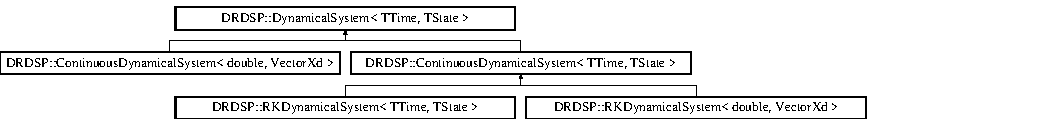
\includegraphics[height=1.577465cm]{struct_d_r_d_s_p_1_1_dynamical_system}
\end{center}
\end{figure}
\subsection*{Public Member Functions}
\begin{DoxyCompactItemize}
\item 
\hypertarget{struct_d_r_d_s_p_1_1_dynamical_system_ab877e883970210e09051f389203fb3e4}{virtual void {\bfseries Advance} (T\-Time dt)=0}\label{struct_d_r_d_s_p_1_1_dynamical_system_ab877e883970210e09051f389203fb3e4}

\end{DoxyCompactItemize}
\subsection*{Public Attributes}
\begin{DoxyCompactItemize}
\item 
\hypertarget{struct_d_r_d_s_p_1_1_dynamical_system_a31ddd60e00edcbe16c980e302b7752de}{T\-State {\bfseries state}}\label{struct_d_r_d_s_p_1_1_dynamical_system_a31ddd60e00edcbe16c980e302b7752de}

\end{DoxyCompactItemize}


The documentation for this struct was generated from the following file\-:\begin{DoxyCompactItemize}
\item 
include/\-D\-R\-D\-S\-P/dynamics/dynamical\-System.\-h\end{DoxyCompactItemize}

\hypertarget{struct_d_r_d_s_p_1_1_embedding}{\section{D\-R\-D\-S\-P\-:\-:Embedding Struct Reference}
\label{struct_d_r_d_s_p_1_1_embedding}\index{D\-R\-D\-S\-P\-::\-Embedding@{D\-R\-D\-S\-P\-::\-Embedding}}
}


Base for an embedding of a state space into R$^\wedge$n.  




{\ttfamily \#include $<$embedding.\-h$>$}

Inheritance diagram for D\-R\-D\-S\-P\-:\-:Embedding\-:\begin{figure}[H]
\begin{center}
\leavevmode
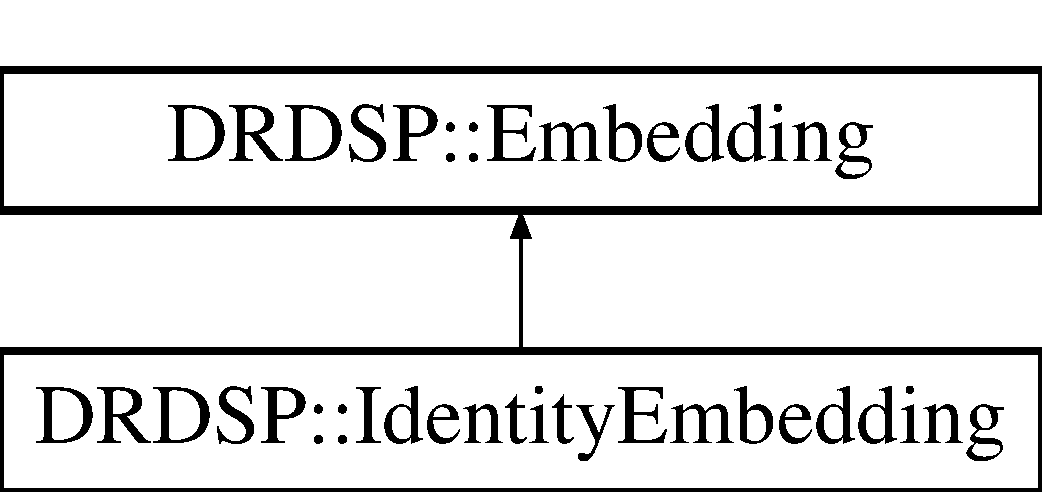
\includegraphics[height=2.000000cm]{struct_d_r_d_s_p_1_1_embedding}
\end{center}
\end{figure}
\subsection*{Public Member Functions}
\begin{DoxyCompactItemize}
\item 
\hypertarget{struct_d_r_d_s_p_1_1_embedding_a761628175adca44353dfae4c5adabe1f}{{\bfseries Embedding} (uint32\-\_\-t \hyperlink{struct_d_r_d_s_p_1_1_embedding_a31e1f302b771269d2475538dc0d12e26}{source\-Dim}, uint32\-\_\-t \hyperlink{struct_d_r_d_s_p_1_1_embedding_a43679793e6c6df0de8a564c97b774928}{embed\-Dim})}\label{struct_d_r_d_s_p_1_1_embedding_a761628175adca44353dfae4c5adabe1f}

\end{DoxyCompactItemize}
\subsection*{Public Attributes}
\begin{DoxyCompactItemize}
\item 
\hypertarget{struct_d_r_d_s_p_1_1_embedding_a31e1f302b771269d2475538dc0d12e26}{uint32\-\_\-t \hyperlink{struct_d_r_d_s_p_1_1_embedding_a31e1f302b771269d2475538dc0d12e26}{source\-Dim}}\label{struct_d_r_d_s_p_1_1_embedding_a31e1f302b771269d2475538dc0d12e26}

\begin{DoxyCompactList}\small\item\em Dimension of the original state space. \end{DoxyCompactList}\item 
\hypertarget{struct_d_r_d_s_p_1_1_embedding_a43679793e6c6df0de8a564c97b774928}{uint32\-\_\-t \hyperlink{struct_d_r_d_s_p_1_1_embedding_a43679793e6c6df0de8a564c97b774928}{embed\-Dim}}\label{struct_d_r_d_s_p_1_1_embedding_a43679793e6c6df0de8a564c97b774928}

\begin{DoxyCompactList}\small\item\em Dimension of the embedding space, R$^\wedge$n. \end{DoxyCompactList}\end{DoxyCompactItemize}


\subsection{Detailed Description}
Base for an embedding of a state space into R$^\wedge$n. 

The documentation for this struct was generated from the following file\-:\begin{DoxyCompactItemize}
\item 
include/\-D\-R\-D\-S\-P/dynamics/embedding.\-h\end{DoxyCompactItemize}

\hypertarget{struct_d_r_d_s_p_1_1_embedding_c_w}{\section{D\-R\-D\-S\-P\-:\-:Embedding\-C\-W Struct Reference}
\label{struct_d_r_d_s_p_1_1_embedding_c_w}\index{D\-R\-D\-S\-P\-::\-Embedding\-C\-W@{D\-R\-D\-S\-P\-::\-Embedding\-C\-W}}
}
\subsection*{Public Member Functions}
\begin{DoxyCompactItemize}
\item 
\hypertarget{struct_d_r_d_s_p_1_1_embedding_c_w_a36beb21857003df4f283dd1f0459b178}{{\bfseries Embedding\-C\-W} (uint32\-\_\-t orig\-Dim, uint32\-\_\-t embed\-Dim)}\label{struct_d_r_d_s_p_1_1_embedding_c_w_a36beb21857003df4f283dd1f0459b178}

\item 
\hypertarget{struct_d_r_d_s_p_1_1_embedding_c_w_a630cb32ea4cf52cc278c89322a944257}{virtual Vector\-Xd {\bfseries Evaluate} (const Vector\-Xd \&x) const }\label{struct_d_r_d_s_p_1_1_embedding_c_w_a630cb32ea4cf52cc278c89322a944257}

\item 
\hypertarget{struct_d_r_d_s_p_1_1_embedding_c_w_ae7e3c46b785e7b023119238a0d8cc0db}{virtual double {\bfseries Derivative} (const Vector\-Xd \&x, uint32\-\_\-t i, uint32\-\_\-t j) const }\label{struct_d_r_d_s_p_1_1_embedding_c_w_ae7e3c46b785e7b023119238a0d8cc0db}

\item 
\hypertarget{struct_d_r_d_s_p_1_1_embedding_c_w_a0350d8d148c7816ae8b2ee27bf4f54cd}{virtual double {\bfseries Derivative\-Adjoint} (const Vector\-Xd \&x, uint32\-\_\-t i, uint32\-\_\-t j) const }\label{struct_d_r_d_s_p_1_1_embedding_c_w_a0350d8d148c7816ae8b2ee27bf4f54cd}

\item 
\hypertarget{struct_d_r_d_s_p_1_1_embedding_c_w_a98b06fcd2b37246b967ff2660be15568}{virtual double {\bfseries Derivative2} (const Vector\-Xd \&x, uint32\-\_\-t i, uint32\-\_\-t j, uint32\-\_\-t k) const }\label{struct_d_r_d_s_p_1_1_embedding_c_w_a98b06fcd2b37246b967ff2660be15568}

\item 
\hypertarget{struct_d_r_d_s_p_1_1_embedding_c_w_a7fc6f574011396ef14a775e02fb7ef25}{double {\bfseries Compute\-Induced\-Metric} (const Vector\-Xd \&x, uint32\-\_\-t i, uint32\-\_\-t j) const }\label{struct_d_r_d_s_p_1_1_embedding_c_w_a7fc6f574011396ef14a775e02fb7ef25}

\item 
\hypertarget{struct_d_r_d_s_p_1_1_embedding_c_w_ad63dfe0eeab18767684e46cd3000ef83}{\hyperlink{struct_d_r_d_s_p_1_1_data_set}{Data\-Set} {\bfseries Embed\-Data} (const \hyperlink{struct_d_r_d_s_p_1_1_data_set}{Data\-Set} \&data) const }\label{struct_d_r_d_s_p_1_1_embedding_c_w_ad63dfe0eeab18767684e46cd3000ef83}

\item 
\hypertarget{struct_d_r_d_s_p_1_1_embedding_c_w_a3ac7659dca082002fef531dd9403ee1f}{\hyperlink{struct_d_r_d_s_p_1_1_data_system}{Data\-System} {\bfseries Embed\-Data} (const \hyperlink{struct_d_r_d_s_p_1_1_data_system}{Data\-System} \&data) const }\label{struct_d_r_d_s_p_1_1_embedding_c_w_a3ac7659dca082002fef531dd9403ee1f}

\end{DoxyCompactItemize}
\subsection*{Public Attributes}
\begin{DoxyCompactItemize}
\item 
\hypertarget{struct_d_r_d_s_p_1_1_embedding_c_w_aa3f8538fb8f9341f744f79a2bda8d8ef}{uint32\-\_\-t {\bfseries o\-Dim}}\label{struct_d_r_d_s_p_1_1_embedding_c_w_aa3f8538fb8f9341f744f79a2bda8d8ef}

\item 
\hypertarget{struct_d_r_d_s_p_1_1_embedding_c_w_ade05f2b8835edeb8b418bcd27d2d74db}{uint32\-\_\-t {\bfseries e\-Dim}}\label{struct_d_r_d_s_p_1_1_embedding_c_w_ade05f2b8835edeb8b418bcd27d2d74db}

\end{DoxyCompactItemize}


The documentation for this struct was generated from the following files\-:\begin{DoxyCompactItemize}
\item 
include/\-D\-R\-D\-S\-P/dynamics/embedding.\-h\item 
src/dynamics/embedding.\-cpp\end{DoxyCompactItemize}

\hypertarget{struct_d_r_d_s_p_1_1_euler}{\section{D\-R\-D\-S\-P\-:\-:Euler$<$ T\-Time, T\-State $>$ Struct Template Reference}
\label{struct_d_r_d_s_p_1_1_euler}\index{D\-R\-D\-S\-P\-::\-Euler$<$ T\-Time, T\-State $>$@{D\-R\-D\-S\-P\-::\-Euler$<$ T\-Time, T\-State $>$}}
}
Inheritance diagram for D\-R\-D\-S\-P\-:\-:Euler$<$ T\-Time, T\-State $>$\-:\begin{figure}[H]
\begin{center}
\leavevmode
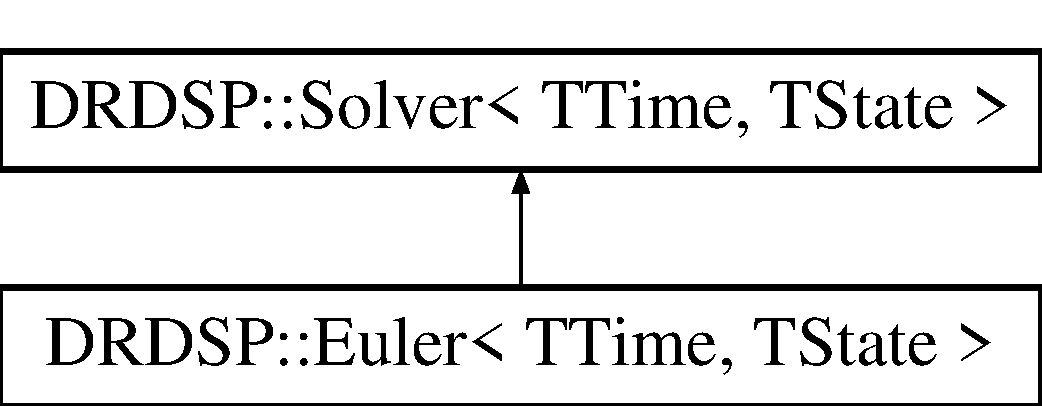
\includegraphics[height=2.000000cm]{struct_d_r_d_s_p_1_1_euler}
\end{center}
\end{figure}
\subsection*{Public Member Functions}
\begin{DoxyCompactItemize}
\item 
\hypertarget{struct_d_r_d_s_p_1_1_euler_acb158bee2c2c68dc9fbd697375b7c5c9}{void {\bfseries Integrate} (T\-State \&x, T\-Time \&t, T\-Time dt)}\label{struct_d_r_d_s_p_1_1_euler_acb158bee2c2c68dc9fbd697375b7c5c9}

\end{DoxyCompactItemize}
\subsection*{Additional Inherited Members}


The documentation for this struct was generated from the following file\-:\begin{DoxyCompactItemize}
\item 
include/\-D\-R\-D\-S\-P/dynamics/solver.\-h\end{DoxyCompactItemize}

\hypertarget{struct_d_r_d_s_p_1_1_function}{\section{D\-R\-D\-S\-P\-:\-:Function Struct Reference}
\label{struct_d_r_d_s_p_1_1_function}\index{D\-R\-D\-S\-P\-::\-Function@{D\-R\-D\-S\-P\-::\-Function}}
}
Inheritance diagram for D\-R\-D\-S\-P\-:\-:Function\-:\begin{figure}[H]
\begin{center}
\leavevmode
\includegraphics[height=0.987654cm]{struct_d_r_d_s_p_1_1_function}
\end{center}
\end{figure}
\subsection*{Public Member Functions}
\begin{DoxyCompactItemize}
\item 
\hypertarget{struct_d_r_d_s_p_1_1_function_ab8c577c9d6cbcf89ae2da9092aaee7b6}{virtual double {\bfseries operator()} (double r) const =0}\label{struct_d_r_d_s_p_1_1_function_ab8c577c9d6cbcf89ae2da9092aaee7b6}

\item 
\hypertarget{struct_d_r_d_s_p_1_1_function_ac01b334d7ca8042e51c703760dc0a243}{virtual double {\bfseries Derivative} (double r) const =0}\label{struct_d_r_d_s_p_1_1_function_ac01b334d7ca8042e51c703760dc0a243}

\end{DoxyCompactItemize}


The documentation for this struct was generated from the following file\-:\begin{DoxyCompactItemize}
\item 
include/\-D\-R\-D\-S\-P/dynamics/radial\-\_\-basis.\-h\end{DoxyCompactItemize}

\hypertarget{struct_d_r_d_s_p_1_1_gaussian}{\section{D\-R\-D\-S\-P\-:\-:Gaussian Struct Reference}
\label{struct_d_r_d_s_p_1_1_gaussian}\index{D\-R\-D\-S\-P\-::\-Gaussian@{D\-R\-D\-S\-P\-::\-Gaussian}}
}
\subsection*{Public Member Functions}
\begin{DoxyCompactItemize}
\item 
\hypertarget{struct_d_r_d_s_p_1_1_gaussian_aff703aa9e683cce46f56a41d173d2643}{double {\bfseries operator()} (double r) const }\label{struct_d_r_d_s_p_1_1_gaussian_aff703aa9e683cce46f56a41d173d2643}

\item 
\hypertarget{struct_d_r_d_s_p_1_1_gaussian_a9ae975cdc5b2bbc1ae2e1c3725f48890}{double {\bfseries Derivative} (double r) const }\label{struct_d_r_d_s_p_1_1_gaussian_a9ae975cdc5b2bbc1ae2e1c3725f48890}

\end{DoxyCompactItemize}
\subsection*{Public Attributes}
\begin{DoxyCompactItemize}
\item 
\hypertarget{struct_d_r_d_s_p_1_1_gaussian_a54c0ec40d9295e0167e6216912f01d2a}{double {\bfseries scale}}\label{struct_d_r_d_s_p_1_1_gaussian_a54c0ec40d9295e0167e6216912f01d2a}

\end{DoxyCompactItemize}


The documentation for this struct was generated from the following files\-:\begin{DoxyCompactItemize}
\item 
include/\-D\-R\-D\-S\-P/dynamics/radial\-\_\-basis.\-h\item 
src/dynamics/radial\-\_\-basis.\-cpp\end{DoxyCompactItemize}

\hypertarget{struct_d_r_d_s_p_1_1_geodesic}{\section{D\-R\-D\-S\-P\-:\-:Geodesic$<$ T\-Vec $>$ Struct Template Reference}
\label{struct_d_r_d_s_p_1_1_geodesic}\index{D\-R\-D\-S\-P\-::\-Geodesic$<$ T\-Vec $>$@{D\-R\-D\-S\-P\-::\-Geodesic$<$ T\-Vec $>$}}
}
\subsection*{Public Member Functions}
\begin{DoxyCompactItemize}
\item 
\hypertarget{struct_d_r_d_s_p_1_1_geodesic_adbe5b874998ae05965c4743d05f9d9f2}{virtual void {\bfseries Set} (const T\-Vec \&point, const T\-Vec \&tangent)}\label{struct_d_r_d_s_p_1_1_geodesic_adbe5b874998ae05965c4743d05f9d9f2}

\item 
\hypertarget{struct_d_r_d_s_p_1_1_geodesic_a7c9365578a93c484a762d00b8326ea4f}{const T\-Vec \& {\bfseries Get\-Point} () const }\label{struct_d_r_d_s_p_1_1_geodesic_a7c9365578a93c484a762d00b8326ea4f}

\item 
\hypertarget{struct_d_r_d_s_p_1_1_geodesic_abe5e93e0cadb4cf672c34857e6eb776a}{const T\-Vec \& {\bfseries Get\-Tangent} () const }\label{struct_d_r_d_s_p_1_1_geodesic_abe5e93e0cadb4cf672c34857e6eb776a}

\item 
\hypertarget{struct_d_r_d_s_p_1_1_geodesic_a7151a62079dd6aee49c5ee572aa9f659}{virtual T\-Vec {\bfseries Evaluate} (double t)}\label{struct_d_r_d_s_p_1_1_geodesic_a7151a62079dd6aee49c5ee572aa9f659}

\item 
\hypertarget{struct_d_r_d_s_p_1_1_geodesic_a72765c1bb3c224bc3f738863c85bab46}{virtual T\-Vec {\bfseries Parallel\-Translate} (const T\-Vec \&V, double t)}\label{struct_d_r_d_s_p_1_1_geodesic_a72765c1bb3c224bc3f738863c85bab46}

\end{DoxyCompactItemize}
\subsection*{Protected Attributes}
\begin{DoxyCompactItemize}
\item 
\hypertarget{struct_d_r_d_s_p_1_1_geodesic_a22554954743fb723aba0255edd316a44}{T\-Vec {\bfseries Point}}\label{struct_d_r_d_s_p_1_1_geodesic_a22554954743fb723aba0255edd316a44}

\item 
\hypertarget{struct_d_r_d_s_p_1_1_geodesic_a7a645623e8edc301cfdebf163cc619ef}{T\-Vec {\bfseries Tangent}}\label{struct_d_r_d_s_p_1_1_geodesic_a7a645623e8edc301cfdebf163cc619ef}

\end{DoxyCompactItemize}


The documentation for this struct was generated from the following file\-:\begin{DoxyCompactItemize}
\item 
include/\-D\-R\-D\-S\-P/geometry/geodesic.\-h\end{DoxyCompactItemize}

\hypertarget{struct_d_r_d_s_p_1_1_gradient_descent}{\section{D\-R\-D\-S\-P\-:\-:Gradient\-Descent$<$ Geodesic $>$ Struct Template Reference}
\label{struct_d_r_d_s_p_1_1_gradient_descent}\index{D\-R\-D\-S\-P\-::\-Gradient\-Descent$<$ Geodesic $>$@{D\-R\-D\-S\-P\-::\-Gradient\-Descent$<$ Geodesic $>$}}
}
\subsection*{Public Types}
\begin{DoxyCompactItemize}
\item 
\hypertarget{struct_d_r_d_s_p_1_1_gradient_descent_a0534fdca2e58308db1766b72510da64a}{typedef Geodesic\-::\-Metric {\bfseries Metric}}\label{struct_d_r_d_s_p_1_1_gradient_descent_a0534fdca2e58308db1766b72510da64a}

\item 
\hypertarget{struct_d_r_d_s_p_1_1_gradient_descent_a35bcc6491682744ad9720510a1d13ecb}{typedef Metric\-::\-Point {\bfseries Point}}\label{struct_d_r_d_s_p_1_1_gradient_descent_a35bcc6491682744ad9720510a1d13ecb}

\end{DoxyCompactItemize}
\subsection*{Public Member Functions}
\begin{DoxyCompactItemize}
\item 
\hypertarget{struct_d_r_d_s_p_1_1_gradient_descent_a826130f2adf7029ab248d9fc4d70d224}{{\footnotesize template$<$typename S , typename D\-S $>$ }\\bool {\bfseries Step} (Point \&x, const S \&cost, const D\-S \&gradient)}\label{struct_d_r_d_s_p_1_1_gradient_descent_a826130f2adf7029ab248d9fc4d70d224}

\item 
\hypertarget{struct_d_r_d_s_p_1_1_gradient_descent_aef8ad1b92b8fefa8f67072f052dfb042}{{\footnotesize template$<$typename S , typename D\-S $>$ }\\bool {\bfseries Optimize} (Point \&x, const S \&cost, const D\-S \&gradient)}\label{struct_d_r_d_s_p_1_1_gradient_descent_aef8ad1b92b8fefa8f67072f052dfb042}

\end{DoxyCompactItemize}
\subsection*{Public Attributes}
\begin{DoxyCompactItemize}
\item 
\hypertarget{struct_d_r_d_s_p_1_1_gradient_descent_a3d83fb182690e94d667cf7e079706427}{Metric {\bfseries metric}}\label{struct_d_r_d_s_p_1_1_gradient_descent_a3d83fb182690e94d667cf7e079706427}

\item 
\hypertarget{struct_d_r_d_s_p_1_1_gradient_descent_a5da80c1f920af9fca7bbee2e4698848b}{\hyperlink{struct_d_r_d_s_p_1_1_line_search}{Line\-Search} {\bfseries line\-Search}}\label{struct_d_r_d_s_p_1_1_gradient_descent_a5da80c1f920af9fca7bbee2e4698848b}

\item 
\hypertarget{struct_d_r_d_s_p_1_1_gradient_descent_afd2cba8ba783cebeb2abd470242c4d5c}{uint32\-\_\-t {\bfseries max\-Steps}}\label{struct_d_r_d_s_p_1_1_gradient_descent_afd2cba8ba783cebeb2abd470242c4d5c}

\end{DoxyCompactItemize}


The documentation for this struct was generated from the following file\-:\begin{DoxyCompactItemize}
\item 
include/\-D\-R\-D\-S\-P/optimization/gradient\-\_\-descent.\-h\end{DoxyCompactItemize}

\hypertarget{struct_d_r_d_s_p_1_1_grassmannian}{\section{D\-R\-D\-S\-P\-:\-:Grassmannian Struct Reference}
\label{struct_d_r_d_s_p_1_1_grassmannian}\index{D\-R\-D\-S\-P\-::\-Grassmannian@{D\-R\-D\-S\-P\-::\-Grassmannian}}
}
Inheritance diagram for D\-R\-D\-S\-P\-:\-:Grassmannian\-:\begin{figure}[H]
\begin{center}
\leavevmode
\includegraphics[height=2.000000cm]{struct_d_r_d_s_p_1_1_grassmannian}
\end{center}
\end{figure}
\subsection*{Public Member Functions}
\begin{DoxyCompactItemize}
\item 
\hypertarget{struct_d_r_d_s_p_1_1_grassmannian_ae287de05dd2c87cc5a9bf3c3546e234b}{void {\bfseries Set} (const Matrix\-Xd \&point, const Matrix\-Xd \&tangent)}\label{struct_d_r_d_s_p_1_1_grassmannian_ae287de05dd2c87cc5a9bf3c3546e234b}

\item 
\hypertarget{struct_d_r_d_s_p_1_1_grassmannian_ab21eaf2cb5b01abe7801fa073179ef0c}{Matrix\-Xd {\bfseries Evaluate} (double t)}\label{struct_d_r_d_s_p_1_1_grassmannian_ab21eaf2cb5b01abe7801fa073179ef0c}

\item 
\hypertarget{struct_d_r_d_s_p_1_1_grassmannian_a7e6d630608028cf6738b24abbbf44ca4}{Matrix\-Xd {\bfseries Parallel\-Translate} (const Matrix\-Xd \&V, double t)}\label{struct_d_r_d_s_p_1_1_grassmannian_a7e6d630608028cf6738b24abbbf44ca4}

\end{DoxyCompactItemize}
\subsection*{Static Public Member Functions}
\begin{DoxyCompactItemize}
\item 
\hypertarget{struct_d_r_d_s_p_1_1_grassmannian_a0430d94764664fbeb8bd97e3d4514082}{static Matrix\-Xd {\bfseries Horizontal\-Component} (const Matrix\-Xd \&W, const Matrix\-Xd \&V)}\label{struct_d_r_d_s_p_1_1_grassmannian_a0430d94764664fbeb8bd97e3d4514082}

\item 
\hypertarget{struct_d_r_d_s_p_1_1_grassmannian_af3ba1867c912e3dc2418b12b54e1f4e5}{static Matrix\-Xd {\bfseries Vertical\-Component} (const Matrix\-Xd \&W, const Matrix\-Xd \&V)}\label{struct_d_r_d_s_p_1_1_grassmannian_af3ba1867c912e3dc2418b12b54e1f4e5}

\end{DoxyCompactItemize}
\subsection*{Protected Types}
\begin{DoxyCompactItemize}
\item 
\hypertarget{struct_d_r_d_s_p_1_1_grassmannian_a23da554a1095a655265e45eed30d7327}{typedef Jacobi\-S\-V\-D$<$ Matrix\-Xd $>$\\*
\-::Singular\-Values\-Type {\bfseries sv\-Type}}\label{struct_d_r_d_s_p_1_1_grassmannian_a23da554a1095a655265e45eed30d7327}

\end{DoxyCompactItemize}
\subsection*{Protected Attributes}
\begin{DoxyCompactItemize}
\item 
\hypertarget{struct_d_r_d_s_p_1_1_grassmannian_a8086c9fce12db9b15634d9d587cd056d}{Jacobi\-S\-V\-D$<$ Matrix\-Xd $>$ {\bfseries svd}}\label{struct_d_r_d_s_p_1_1_grassmannian_a8086c9fce12db9b15634d9d587cd056d}

\end{DoxyCompactItemize}


The documentation for this struct was generated from the following files\-:\begin{DoxyCompactItemize}
\item 
include/\-D\-R\-D\-S\-P/geometry/grassmannian.\-h\item 
src/geometry/grassmannian.\-cpp\end{DoxyCompactItemize}

\hypertarget{struct_d_r_d_s_p_1_1_histogram}{\section{D\-R\-D\-S\-P\-:\-:Histogram Struct Reference}
\label{struct_d_r_d_s_p_1_1_histogram}\index{D\-R\-D\-S\-P\-::\-Histogram@{D\-R\-D\-S\-P\-::\-Histogram}}
}


A histogram.  




{\ttfamily \#include $<$histogram.\-h$>$}

\subsection*{Public Member Functions}
\begin{DoxyCompactItemize}
\item 
\hypertarget{struct_d_r_d_s_p_1_1_histogram_a5555b96af544fc87151196d59d83c20a}{{\bfseries Histogram} (uint32\-\_\-t n\-Bins)}\label{struct_d_r_d_s_p_1_1_histogram_a5555b96af544fc87151196d59d83c20a}

\item 
\hypertarget{struct_d_r_d_s_p_1_1_histogram_a11252e6e91d54a93766eab33756e46fd}{void {\bfseries Create} (uint32\-\_\-t n\-Bins)}\label{struct_d_r_d_s_p_1_1_histogram_a11252e6e91d54a93766eab33756e46fd}

\item 
\hypertarget{struct_d_r_d_s_p_1_1_histogram_a84577ee394d1017b16aa4229ff7f5904}{void {\bfseries Destroy} ()}\label{struct_d_r_d_s_p_1_1_histogram_a84577ee394d1017b16aa4229ff7f5904}

\item 
\hypertarget{struct_d_r_d_s_p_1_1_histogram_adeb7a588aa66fe2e6dd0d851ea92d625}{uint32\-\_\-t \hyperlink{struct_d_r_d_s_p_1_1_histogram_adeb7a588aa66fe2e6dd0d851ea92d625}{Total\-Frequency} () const }\label{struct_d_r_d_s_p_1_1_histogram_adeb7a588aa66fe2e6dd0d851ea92d625}

\begin{DoxyCompactList}\small\item\em Sums the bin frequencies. \end{DoxyCompactList}\item 
\hypertarget{struct_d_r_d_s_p_1_1_histogram_a849de9ad07ff6c468dad15a9951a3f81}{void {\bfseries Write\-C\-S\-V} (const char $\ast$filename) const }\label{struct_d_r_d_s_p_1_1_histogram_a849de9ad07ff6c468dad15a9951a3f81}

\end{DoxyCompactItemize}
\subsection*{Public Attributes}
\begin{DoxyCompactItemize}
\item 
\hypertarget{struct_d_r_d_s_p_1_1_histogram_af08514f760ecf60c8ccd422e38bd98cc}{vector$<$ \hyperlink{struct_d_r_d_s_p_1_1_bin}{Bin} $>$ {\bfseries bins}}\label{struct_d_r_d_s_p_1_1_histogram_af08514f760ecf60c8ccd422e38bd98cc}

\end{DoxyCompactItemize}


\subsection{Detailed Description}
A histogram. 

This is just an array of bins with some helper functions. 

The documentation for this struct was generated from the following files\-:\begin{DoxyCompactItemize}
\item 
include/\-D\-R\-D\-S\-P/data/histogram.\-h\item 
src/data/histogram.\-cpp\end{DoxyCompactItemize}

\hypertarget{struct_d_r_d_s_p_1_1_histogram_generator}{\section{D\-R\-D\-S\-P\-:\-:Histogram\-Generator Struct Reference}
\label{struct_d_r_d_s_p_1_1_histogram_generator}\index{D\-R\-D\-S\-P\-::\-Histogram\-Generator@{D\-R\-D\-S\-P\-::\-Histogram\-Generator}}
}


A class for generating histograms from data.  




{\ttfamily \#include $<$histogram.\-h$>$}

\subsection*{Public Member Functions}
\begin{DoxyCompactItemize}
\item 
\hypertarget{struct_d_r_d_s_p_1_1_histogram_generator_aba084569d244397f561b0f219921d296}{\hyperlink{struct_d_r_d_s_p_1_1_histogram_generator_aba084569d244397f561b0f219921d296}{Histogram\-Generator} ()}\label{struct_d_r_d_s_p_1_1_histogram_generator_aba084569d244397f561b0f219921d296}

\begin{DoxyCompactList}\small\item\em Use a logarithmic scale for the bin sizes. \end{DoxyCompactList}\item 
\hypertarget{struct_d_r_d_s_p_1_1_histogram_generator_ad8a1d610f8fb2ca15b3765d54e13885e}{{\bfseries Histogram\-Generator} (uint32\-\_\-t n\-Bins)}\label{struct_d_r_d_s_p_1_1_histogram_generator_ad8a1d610f8fb2ca15b3765d54e13885e}

\item 
\hypertarget{struct_d_r_d_s_p_1_1_histogram_generator_af1acac305990b01bc4cc6e612415bf72}{\hyperlink{struct_d_r_d_s_p_1_1_histogram}{Histogram} {\bfseries Generate} (const double $\ast$data, size\-\_\-t N) const }\label{struct_d_r_d_s_p_1_1_histogram_generator_af1acac305990b01bc4cc6e612415bf72}

\end{DoxyCompactItemize}
\subsection*{Public Attributes}
\begin{DoxyCompactItemize}
\item 
\hypertarget{struct_d_r_d_s_p_1_1_histogram_generator_a2f6b01668e743ce436f54c3ca56275a1}{uint32\-\_\-t {\bfseries num\-Bins}}\label{struct_d_r_d_s_p_1_1_histogram_generator_a2f6b01668e743ce436f54c3ca56275a1}

\item 
\hypertarget{struct_d_r_d_s_p_1_1_histogram_generator_aef85198c4644dbcfa27d24e9015bb025}{double \hyperlink{struct_d_r_d_s_p_1_1_histogram_generator_aef85198c4644dbcfa27d24e9015bb025}{clamp\-Min}}\label{struct_d_r_d_s_p_1_1_histogram_generator_aef85198c4644dbcfa27d24e9015bb025}

\begin{DoxyCompactList}\small\item\em The number of bins that we want the histogram to contain. \end{DoxyCompactList}\item 
\hypertarget{struct_d_r_d_s_p_1_1_histogram_generator_a5cec8e7e75d95a66b4a17c3f70c2b556}{double {\bfseries clamp\-Max}}\label{struct_d_r_d_s_p_1_1_histogram_generator_a5cec8e7e75d95a66b4a17c3f70c2b556}

\item 
\hypertarget{struct_d_r_d_s_p_1_1_histogram_generator_a12fe0ce6860a6f8bd17b1355f91c0ac6}{bool \hyperlink{struct_d_r_d_s_p_1_1_histogram_generator_a12fe0ce6860a6f8bd17b1355f91c0ac6}{clamp}}\label{struct_d_r_d_s_p_1_1_histogram_generator_a12fe0ce6860a6f8bd17b1355f91c0ac6}

\begin{DoxyCompactList}\small\item\em clamping limits the range of the bins \end{DoxyCompactList}\item 
\hypertarget{struct_d_r_d_s_p_1_1_histogram_generator_a84935b50902a985afdeca6541bac8c06}{bool \hyperlink{struct_d_r_d_s_p_1_1_histogram_generator_a84935b50902a985afdeca6541bac8c06}{log\-Scale}}\label{struct_d_r_d_s_p_1_1_histogram_generator_a84935b50902a985afdeca6541bac8c06}

\begin{DoxyCompactList}\small\item\em Perform clamping. \end{DoxyCompactList}\end{DoxyCompactItemize}


\subsection{Detailed Description}
A class for generating histograms from data. 

The documentation for this struct was generated from the following files\-:\begin{DoxyCompactItemize}
\item 
include/\-D\-R\-D\-S\-P/data/histogram.\-h\item 
src/data/histogram.\-cpp\end{DoxyCompactItemize}

\hypertarget{struct_d_r_d_s_p_1_1_inner_product}{\section{D\-R\-D\-S\-P\-:\-:Inner\-Product$<$ Derived $>$ Struct Template Reference}
\label{struct_d_r_d_s_p_1_1_inner_product}\index{D\-R\-D\-S\-P\-::\-Inner\-Product$<$ Derived $>$@{D\-R\-D\-S\-P\-::\-Inner\-Product$<$ Derived $>$}}
}
\subsection*{Public Types}
\begin{DoxyCompactItemize}
\item 
\hypertarget{struct_d_r_d_s_p_1_1_inner_product_a17ea87e68e60f51e48a2744e8a46c958}{typedef \hyperlink{struct_d_r_d_s_p_1_1_traits}{Traits}$<$ Derived $>$\-::T\-Vec {\bfseries T\-Vec}}\label{struct_d_r_d_s_p_1_1_inner_product_a17ea87e68e60f51e48a2744e8a46c958}

\item 
\hypertarget{struct_d_r_d_s_p_1_1_inner_product_af3dad68262d43466e9d3ee914bd70041}{typedef \hyperlink{struct_d_r_d_s_p_1_1_traits}{Traits}$<$ Derived $>$\-::T\-C\-V {\bfseries T\-C\-V}}\label{struct_d_r_d_s_p_1_1_inner_product_af3dad68262d43466e9d3ee914bd70041}

\item 
\hypertarget{struct_d_r_d_s_p_1_1_inner_product_ac4de33c75ca947cc2af0495473dde742}{typedef \hyperlink{struct_d_r_d_s_p_1_1_traits}{Traits}$<$ Derived $>$\-::T\-Scalar {\bfseries T\-Scalar}}\label{struct_d_r_d_s_p_1_1_inner_product_ac4de33c75ca947cc2af0495473dde742}

\end{DoxyCompactItemize}
\subsection*{Public Member Functions}
\begin{DoxyCompactItemize}
\item 
\hypertarget{struct_d_r_d_s_p_1_1_inner_product_a031062be7cf0accf6edcd6f2548551e6}{virtual T\-Scalar {\bfseries operator()} (const T\-Vec \&V, const T\-Vec \&W) const =0}\label{struct_d_r_d_s_p_1_1_inner_product_a031062be7cf0accf6edcd6f2548551e6}

\item 
\hypertarget{struct_d_r_d_s_p_1_1_inner_product_af1060a7d135de0be40781a0f2274b278}{virtual T\-Scalar {\bfseries Norm2} (const T\-Vec \&V) const =0}\label{struct_d_r_d_s_p_1_1_inner_product_af1060a7d135de0be40781a0f2274b278}

\item 
\hypertarget{struct_d_r_d_s_p_1_1_inner_product_a21893f0870c563cb8399b9e8897afa79}{virtual T\-C\-V {\bfseries Flat} (const T\-Vec \&V) const =0}\label{struct_d_r_d_s_p_1_1_inner_product_a21893f0870c563cb8399b9e8897afa79}

\item 
\hypertarget{struct_d_r_d_s_p_1_1_inner_product_a075af7a56185206cd221c93a834bc354}{virtual T\-Vec {\bfseries Sharp} (const T\-C\-V \&V) const =0}\label{struct_d_r_d_s_p_1_1_inner_product_a075af7a56185206cd221c93a834bc354}

\end{DoxyCompactItemize}


The documentation for this struct was generated from the following file\-:\begin{DoxyCompactItemize}
\item 
include/\-D\-R\-D\-S\-P/geometry/inner\-\_\-product.\-h\end{DoxyCompactItemize}

\hypertarget{struct_d_r_d_s_p_1_1_inverse_multiquadratic}{\section{D\-R\-D\-S\-P\-:\-:Inverse\-Multiquadratic Struct Reference}
\label{struct_d_r_d_s_p_1_1_inverse_multiquadratic}\index{D\-R\-D\-S\-P\-::\-Inverse\-Multiquadratic@{D\-R\-D\-S\-P\-::\-Inverse\-Multiquadratic}}
}
\subsection*{Public Member Functions}
\begin{DoxyCompactItemize}
\item 
\hypertarget{struct_d_r_d_s_p_1_1_inverse_multiquadratic_a9de4a748cfda8c1bd8c0dfca408faed7}{{\bfseries Inverse\-Multiquadratic} (double scale)}\label{struct_d_r_d_s_p_1_1_inverse_multiquadratic_a9de4a748cfda8c1bd8c0dfca408faed7}

\item 
\hypertarget{struct_d_r_d_s_p_1_1_inverse_multiquadratic_a513dbe313c51ad9ba2c9397c987563f7}{double {\bfseries operator()} (double r) const }\label{struct_d_r_d_s_p_1_1_inverse_multiquadratic_a513dbe313c51ad9ba2c9397c987563f7}

\item 
\hypertarget{struct_d_r_d_s_p_1_1_inverse_multiquadratic_af6a5298e54581ec417a06335c3757744}{double {\bfseries Derivative} (double r) const }\label{struct_d_r_d_s_p_1_1_inverse_multiquadratic_af6a5298e54581ec417a06335c3757744}

\end{DoxyCompactItemize}
\subsection*{Public Attributes}
\begin{DoxyCompactItemize}
\item 
\hypertarget{struct_d_r_d_s_p_1_1_inverse_multiquadratic_a39009875f833958785889ac9373ad37c}{double {\bfseries scale}}\label{struct_d_r_d_s_p_1_1_inverse_multiquadratic_a39009875f833958785889ac9373ad37c}

\end{DoxyCompactItemize}


The documentation for this struct was generated from the following files\-:\begin{DoxyCompactItemize}
\item 
include/\-D\-R\-D\-S\-P/dynamics/radial\-\_\-basis.\-h\item 
src/dynamics/radial\-\_\-basis.\-cpp\end{DoxyCompactItemize}

\hypertarget{struct_d_r_d_s_p_1_1_inverse_quadratic}{\section{D\-R\-D\-S\-P\-:\-:Inverse\-Quadratic Struct Reference}
\label{struct_d_r_d_s_p_1_1_inverse_quadratic}\index{D\-R\-D\-S\-P\-::\-Inverse\-Quadratic@{D\-R\-D\-S\-P\-::\-Inverse\-Quadratic}}
}
\subsection*{Public Member Functions}
\begin{DoxyCompactItemize}
\item 
\hypertarget{struct_d_r_d_s_p_1_1_inverse_quadratic_a4a7714fcbafbaec4bb30c6922feb59e1}{{\bfseries Inverse\-Quadratic} (double scale)}\label{struct_d_r_d_s_p_1_1_inverse_quadratic_a4a7714fcbafbaec4bb30c6922feb59e1}

\item 
\hypertarget{struct_d_r_d_s_p_1_1_inverse_quadratic_a24a735561bee7c360ee1d1d86126fdad}{{\footnotesize template$<$typename T $>$ }\\T {\bfseries operator()} (T r) const }\label{struct_d_r_d_s_p_1_1_inverse_quadratic_a24a735561bee7c360ee1d1d86126fdad}

\item 
\hypertarget{struct_d_r_d_s_p_1_1_inverse_quadratic_af57547e80e67331d04526fbb98d9bc2c}{{\footnotesize template$<$typename T $>$ }\\T {\bfseries Derivative} (T r) const }\label{struct_d_r_d_s_p_1_1_inverse_quadratic_af57547e80e67331d04526fbb98d9bc2c}

\end{DoxyCompactItemize}
\subsection*{Public Attributes}
\begin{DoxyCompactItemize}
\item 
\hypertarget{struct_d_r_d_s_p_1_1_inverse_quadratic_a31241ecd1ec571b651307d29e6b69c07}{double {\bfseries scale}}\label{struct_d_r_d_s_p_1_1_inverse_quadratic_a31241ecd1ec571b651307d29e6b69c07}

\end{DoxyCompactItemize}


The documentation for this struct was generated from the following file\-:\begin{DoxyCompactItemize}
\item 
include/\-D\-R\-D\-S\-P/dynamics/radial\-\_\-basis.\-h\end{DoxyCompactItemize}

\hypertarget{struct_d_r_d_s_p_1_1_i_p_dot}{\section{D\-R\-D\-S\-P\-:\-:I\-P\-Dot Struct Reference}
\label{struct_d_r_d_s_p_1_1_i_p_dot}\index{D\-R\-D\-S\-P\-::\-I\-P\-Dot@{D\-R\-D\-S\-P\-::\-I\-P\-Dot}}
}
Inheritance diagram for D\-R\-D\-S\-P\-:\-:I\-P\-Dot\-:\begin{figure}[H]
\begin{center}
\leavevmode
\includegraphics[height=2.000000cm]{struct_d_r_d_s_p_1_1_i_p_dot}
\end{center}
\end{figure}
\subsection*{Public Member Functions}
\begin{DoxyCompactItemize}
\item 
\hypertarget{struct_d_r_d_s_p_1_1_i_p_dot_a04fd32a9c8452a39e048bf455bed4704}{T\-Scalar {\bfseries operator()} (const T\-Vec \&V, const T\-Vec \&W) const }\label{struct_d_r_d_s_p_1_1_i_p_dot_a04fd32a9c8452a39e048bf455bed4704}

\item 
\hypertarget{struct_d_r_d_s_p_1_1_i_p_dot_a18e6e71fc6c295234ecd4fe38c3ec0a1}{T\-Scalar {\bfseries Norm2} (const T\-Vec \&V) const }\label{struct_d_r_d_s_p_1_1_i_p_dot_a18e6e71fc6c295234ecd4fe38c3ec0a1}

\item 
\hypertarget{struct_d_r_d_s_p_1_1_i_p_dot_a9401510883e01f0234ed98fae2542504}{T\-C\-V {\bfseries Flat} (const T\-Vec \&V) const }\label{struct_d_r_d_s_p_1_1_i_p_dot_a9401510883e01f0234ed98fae2542504}

\item 
\hypertarget{struct_d_r_d_s_p_1_1_i_p_dot_a2e454edec85353eb6a48eeda553c1a0a}{T\-Vec {\bfseries Sharp} (const T\-C\-V \&V) const }\label{struct_d_r_d_s_p_1_1_i_p_dot_a2e454edec85353eb6a48eeda553c1a0a}

\end{DoxyCompactItemize}
\subsection*{Additional Inherited Members}


The documentation for this struct was generated from the following file\-:\begin{DoxyCompactItemize}
\item 
include/\-D\-R\-D\-S\-P/geometry/inner\-\_\-product.\-h\end{DoxyCompactItemize}

\hypertarget{struct_d_r_d_s_p_1_1_i_p_frobenius}{\section{D\-R\-D\-S\-P\-:\-:I\-P\-Frobenius Struct Reference}
\label{struct_d_r_d_s_p_1_1_i_p_frobenius}\index{D\-R\-D\-S\-P\-::\-I\-P\-Frobenius@{D\-R\-D\-S\-P\-::\-I\-P\-Frobenius}}
}
Inheritance diagram for D\-R\-D\-S\-P\-:\-:I\-P\-Frobenius\-:\begin{figure}[H]
\begin{center}
\leavevmode
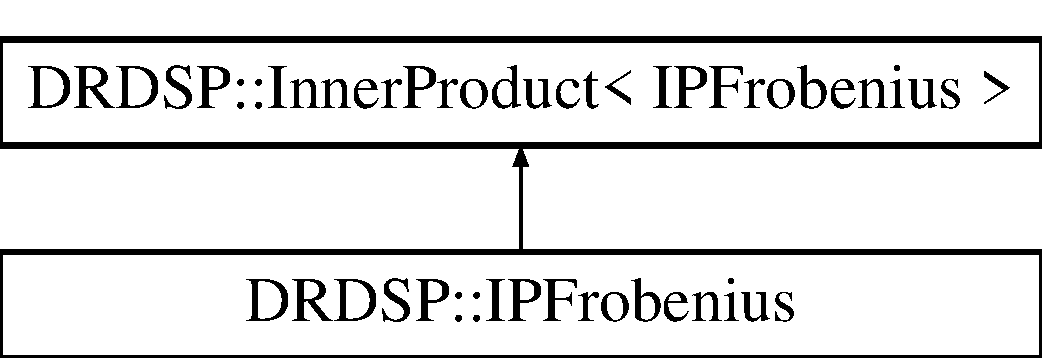
\includegraphics[height=2.000000cm]{struct_d_r_d_s_p_1_1_i_p_frobenius}
\end{center}
\end{figure}
\subsection*{Public Member Functions}
\begin{DoxyCompactItemize}
\item 
\hypertarget{struct_d_r_d_s_p_1_1_i_p_frobenius_a5b88ec43638c497e0199f98ab34aa10e}{T\-Scalar {\bfseries operator()} (const T\-Vec \&V, const T\-Vec \&W) const }\label{struct_d_r_d_s_p_1_1_i_p_frobenius_a5b88ec43638c497e0199f98ab34aa10e}

\item 
\hypertarget{struct_d_r_d_s_p_1_1_i_p_frobenius_a3b7f0fc2c50894fdd0df46ba3315bf0f}{T\-Scalar {\bfseries Norm2} (const T\-Vec \&V) const }\label{struct_d_r_d_s_p_1_1_i_p_frobenius_a3b7f0fc2c50894fdd0df46ba3315bf0f}

\item 
\hypertarget{struct_d_r_d_s_p_1_1_i_p_frobenius_a6fe021cb68fc41f8458731025be7f01e}{T\-C\-V {\bfseries Flat} (const T\-Vec \&V) const }\label{struct_d_r_d_s_p_1_1_i_p_frobenius_a6fe021cb68fc41f8458731025be7f01e}

\item 
\hypertarget{struct_d_r_d_s_p_1_1_i_p_frobenius_ae4baabce6d2b3657e427a44b8b32434e}{T\-Vec {\bfseries Sharp} (const T\-C\-V \&V) const }\label{struct_d_r_d_s_p_1_1_i_p_frobenius_ae4baabce6d2b3657e427a44b8b32434e}

\end{DoxyCompactItemize}
\subsection*{Additional Inherited Members}


The documentation for this struct was generated from the following file\-:\begin{DoxyCompactItemize}
\item 
include/\-D\-R\-D\-S\-P/geometry/inner\-\_\-product.\-h\end{DoxyCompactItemize}

\hypertarget{struct_d_r_d_s_p_1_1_line_search}{\section{D\-R\-D\-S\-P\-:\-:Line\-Search Struct Reference}
\label{struct_d_r_d_s_p_1_1_line_search}\index{D\-R\-D\-S\-P\-::\-Line\-Search@{D\-R\-D\-S\-P\-::\-Line\-Search}}
}
\subsection*{Public Member Functions}
\begin{DoxyCompactItemize}
\item 
\hypertarget{struct_d_r_d_s_p_1_1_line_search_a6bcec01e58efcf7fe7306370de904717}{{\footnotesize template$<$typename S , typename D\-S $>$ }\\double {\bfseries Search} (S \&\&cost, D\-S \&\&cost\-Deriv)}\label{struct_d_r_d_s_p_1_1_line_search_a6bcec01e58efcf7fe7306370de904717}

\end{DoxyCompactItemize}
\subsection*{Public Attributes}
\begin{DoxyCompactItemize}
\item 
\hypertarget{struct_d_r_d_s_p_1_1_line_search_aa1b9be6dd476ea782296caf27fc87bcd}{double {\bfseries alpha}}\label{struct_d_r_d_s_p_1_1_line_search_aa1b9be6dd476ea782296caf27fc87bcd}

\item 
\hypertarget{struct_d_r_d_s_p_1_1_line_search_a79d6f5eaed56fd506b1d8a8f687d54a9}{double {\bfseries alpha\-Max}}\label{struct_d_r_d_s_p_1_1_line_search_a79d6f5eaed56fd506b1d8a8f687d54a9}

\item 
\hypertarget{struct_d_r_d_s_p_1_1_line_search_a48ee96d436216a66de45a13d700fcdaa}{double {\bfseries mu}}\label{struct_d_r_d_s_p_1_1_line_search_a48ee96d436216a66de45a13d700fcdaa}

\item 
\hypertarget{struct_d_r_d_s_p_1_1_line_search_ad1e2b29ad51dd189d3631fad059ec5d9}{double {\bfseries eta}}\label{struct_d_r_d_s_p_1_1_line_search_ad1e2b29ad51dd189d3631fad059ec5d9}

\item 
\hypertarget{struct_d_r_d_s_p_1_1_line_search_a3bb00fed00ecf84072fc6af165be2776}{double {\bfseries S0}}\label{struct_d_r_d_s_p_1_1_line_search_a3bb00fed00ecf84072fc6af165be2776}

\item 
\hypertarget{struct_d_r_d_s_p_1_1_line_search_ad76f45369c080f3d44f1daaf96114fe2}{double {\bfseries D\-S0}}\label{struct_d_r_d_s_p_1_1_line_search_ad76f45369c080f3d44f1daaf96114fe2}

\end{DoxyCompactItemize}
\subsection*{Protected Member Functions}
\begin{DoxyCompactItemize}
\item 
\hypertarget{struct_d_r_d_s_p_1_1_line_search_af19d762879a466e39377b777f4eb15a0}{bool {\bfseries Wolfe} (double Sc, double gc) const }\label{struct_d_r_d_s_p_1_1_line_search_af19d762879a466e39377b777f4eb15a0}

\end{DoxyCompactItemize}
\subsection*{Static Protected Member Functions}
\begin{DoxyCompactItemize}
\item 
\hypertarget{struct_d_r_d_s_p_1_1_line_search_ac744fe4fb4dda7e2c71b97cf4cf162a6}{static double {\bfseries Secant} (double a, double b, double ga, double gb)}\label{struct_d_r_d_s_p_1_1_line_search_ac744fe4fb4dda7e2c71b97cf4cf162a6}

\end{DoxyCompactItemize}


The documentation for this struct was generated from the following file\-:\begin{DoxyCompactItemize}
\item 
include/\-D\-R\-D\-S\-P/optimization/linesearch.\-h\end{DoxyCompactItemize}

\hypertarget{struct_d_r_d_s_p_1_1_metric}{\section{D\-R\-D\-S\-P\-:\-:Metric$<$ Derived $>$ Struct Template Reference}
\label{struct_d_r_d_s_p_1_1_metric}\index{D\-R\-D\-S\-P\-::\-Metric$<$ Derived $>$@{D\-R\-D\-S\-P\-::\-Metric$<$ Derived $>$}}
}
\subsection*{Public Types}
\begin{DoxyCompactItemize}
\item 
\hypertarget{struct_d_r_d_s_p_1_1_metric_af320bd0a4c60f0d80ab886a2a017c1a1}{typedef \hyperlink{struct_d_r_d_s_p_1_1_traits}{Traits}$<$ Derived $>$\-::T\-I\-P {\bfseries T\-I\-P}}\label{struct_d_r_d_s_p_1_1_metric_af320bd0a4c60f0d80ab886a2a017c1a1}

\item 
\hypertarget{struct_d_r_d_s_p_1_1_metric_a8d9c7b616817989b17a2635e6587bd76}{typedef \hyperlink{struct_d_r_d_s_p_1_1_traits}{Traits}$<$ T\-I\-P $>$\-::T\-Vec {\bfseries T\-Vec}}\label{struct_d_r_d_s_p_1_1_metric_a8d9c7b616817989b17a2635e6587bd76}

\end{DoxyCompactItemize}
\subsection*{Public Member Functions}
\begin{DoxyCompactItemize}
\item 
\hypertarget{struct_d_r_d_s_p_1_1_metric_af576d41e6582b058e4251c13195c0caf}{virtual T\-I\-P {\bfseries operator()} (const T\-Vec \&X) const =0}\label{struct_d_r_d_s_p_1_1_metric_af576d41e6582b058e4251c13195c0caf}

\end{DoxyCompactItemize}


The documentation for this struct was generated from the following file\-:\begin{DoxyCompactItemize}
\item 
include/\-D\-R\-D\-S\-P/geometry/metric.\-h\end{DoxyCompactItemize}

\hypertarget{struct_d_r_d_s_p_1_1_metric_uniform}{\section{D\-R\-D\-S\-P\-:\-:Metric\-Uniform$<$ \-\_\-\-T\-I\-P $>$ Struct Template Reference}
\label{struct_d_r_d_s_p_1_1_metric_uniform}\index{D\-R\-D\-S\-P\-::\-Metric\-Uniform$<$ \-\_\-\-T\-I\-P $>$@{D\-R\-D\-S\-P\-::\-Metric\-Uniform$<$ \-\_\-\-T\-I\-P $>$}}
}
Inheritance diagram for D\-R\-D\-S\-P\-:\-:Metric\-Uniform$<$ \-\_\-\-T\-I\-P $>$\-:\begin{figure}[H]
\begin{center}
\leavevmode
\includegraphics[height=2.000000cm]{struct_d_r_d_s_p_1_1_metric_uniform}
\end{center}
\end{figure}
\subsection*{Public Member Functions}
\begin{DoxyCompactItemize}
\item 
\hypertarget{struct_d_r_d_s_p_1_1_metric_uniform_a30c3e100ba28959007af2d2967e61e29}{T\-I\-P {\bfseries operator()} (const T\-Vec \&X) const }\label{struct_d_r_d_s_p_1_1_metric_uniform_a30c3e100ba28959007af2d2967e61e29}

\item 
\hypertarget{struct_d_r_d_s_p_1_1_metric_uniform_a49c7413ee783f5971f7c6c6da69fdd0f}{const T\-I\-P \& {\bfseries operator()} () const }\label{struct_d_r_d_s_p_1_1_metric_uniform_a49c7413ee783f5971f7c6c6da69fdd0f}

\end{DoxyCompactItemize}
\subsection*{Public Attributes}
\begin{DoxyCompactItemize}
\item 
\hypertarget{struct_d_r_d_s_p_1_1_metric_uniform_aaec3c0874b685ac42954f81d8d6d4dee}{T\-I\-P {\bfseries I\-P}}\label{struct_d_r_d_s_p_1_1_metric_uniform_aaec3c0874b685ac42954f81d8d6d4dee}

\end{DoxyCompactItemize}
\subsection*{Additional Inherited Members}


The documentation for this struct was generated from the following file\-:\begin{DoxyCompactItemize}
\item 
include/\-D\-R\-D\-S\-P/geometry/metric.\-h\end{DoxyCompactItemize}

\hypertarget{struct_d_r_d_s_p_1_1_model}{\section{D\-R\-D\-S\-P\-:\-:Model Struct Reference}
\label{struct_d_r_d_s_p_1_1_model}\index{D\-R\-D\-S\-P\-::\-Model@{D\-R\-D\-S\-P\-::\-Model}}
}


Interface for a model without parameters.  




{\ttfamily \#include $<$model.\-h$>$}

Inheritance diagram for D\-R\-D\-S\-P\-:\-:Model\-:\begin{figure}[H]
\begin{center}
\leavevmode
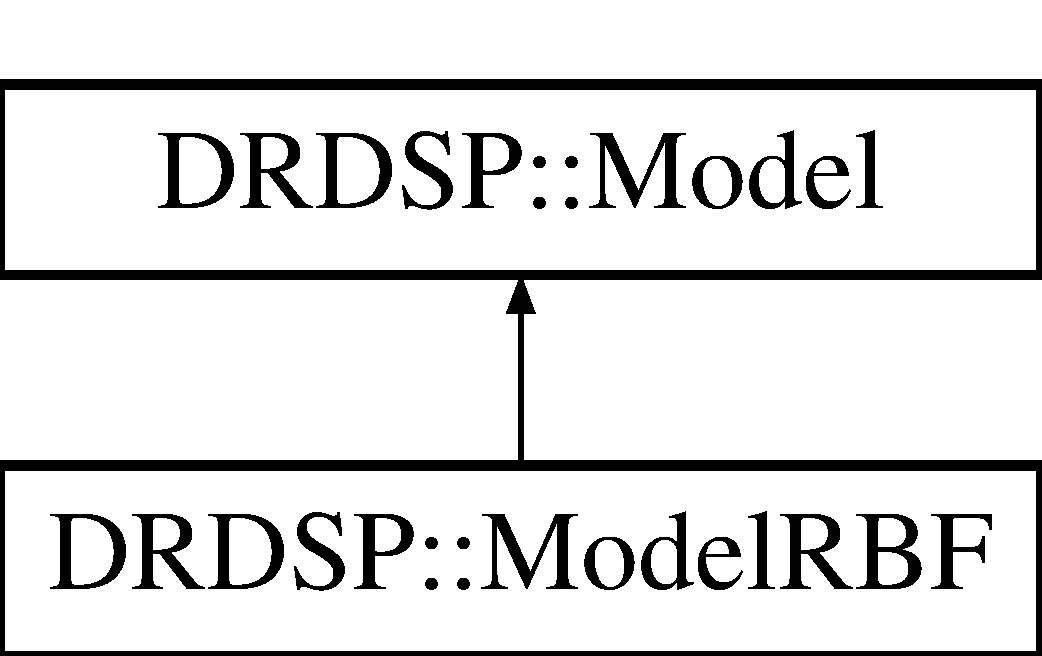
\includegraphics[height=2.000000cm]{struct_d_r_d_s_p_1_1_model}
\end{center}
\end{figure}
\subsection*{Public Member Functions}
\begin{DoxyCompactItemize}
\item 
\hypertarget{struct_d_r_d_s_p_1_1_model_af9ab80237f807fecc435534c8705ea8c}{{\bfseries Model} (const \hyperlink{struct_d_r_d_s_p_1_1_wrap_function}{Wrap\-Function}$<$ Vector\-Xd $>$ $\ast$wrap\-Func)}\label{struct_d_r_d_s_p_1_1_model_af9ab80237f807fecc435534c8705ea8c}

\item 
\hypertarget{struct_d_r_d_s_p_1_1_model_a79dabe991f920ca21ac23066270ab1b7}{{\bfseries Model} (uint32\-\_\-t dim)}\label{struct_d_r_d_s_p_1_1_model_a79dabe991f920ca21ac23066270ab1b7}

\item 
\hypertarget{struct_d_r_d_s_p_1_1_model_a6e682e5b23ddca692c45a3bc6be9dd15}{{\bfseries Model} (const \hyperlink{struct_d_r_d_s_p_1_1_wrap_function}{Wrap\-Function}$<$ Vector\-Xd $>$ $\ast$wrap\-Func, uint32\-\_\-t dim)}\label{struct_d_r_d_s_p_1_1_model_a6e682e5b23ddca692c45a3bc6be9dd15}

\item 
\hypertarget{struct_d_r_d_s_p_1_1_model_a3dd65a7f5c3b1e5e89920a309ff2abec}{virtual Vector\-Xd \hyperlink{struct_d_r_d_s_p_1_1_model_a3dd65a7f5c3b1e5e89920a309ff2abec}{Vector\-Field} (const Vector\-Xd \&state)=0}\label{struct_d_r_d_s_p_1_1_model_a3dd65a7f5c3b1e5e89920a309ff2abec}

\begin{DoxyCompactList}\small\item\em The vector field. \end{DoxyCompactList}\item 
\hypertarget{struct_d_r_d_s_p_1_1_model_a36f5e07d59e484b0ddfc12ed820e55d1}{virtual Matrix\-Xd \hyperlink{struct_d_r_d_s_p_1_1_model_a36f5e07d59e484b0ddfc12ed820e55d1}{Partials} (const Vector\-Xd \&state)=0}\label{struct_d_r_d_s_p_1_1_model_a36f5e07d59e484b0ddfc12ed820e55d1}

\begin{DoxyCompactList}\small\item\em The partial derivatives of the vector field. \end{DoxyCompactList}\end{DoxyCompactItemize}
\subsection*{Public Attributes}
\begin{DoxyCompactItemize}
\item 
\hypertarget{struct_d_r_d_s_p_1_1_model_a286bbeaa673d5e756b1b4e97bdab30f6}{const \hyperlink{struct_d_r_d_s_p_1_1_wrap_function}{Wrap\-Function}$<$ Vector\-Xd $>$ $\ast$ {\bfseries wrap\-Function}}\label{struct_d_r_d_s_p_1_1_model_a286bbeaa673d5e756b1b4e97bdab30f6}

\item 
\hypertarget{struct_d_r_d_s_p_1_1_model_af1e4d4ae5a0dec4460845a58dbd312e9}{uint32\-\_\-t \hyperlink{struct_d_r_d_s_p_1_1_model_af1e4d4ae5a0dec4460845a58dbd312e9}{dimension}}\label{struct_d_r_d_s_p_1_1_model_af1e4d4ae5a0dec4460845a58dbd312e9}

\begin{DoxyCompactList}\small\item\em Dimension of the model's state space. \end{DoxyCompactList}\end{DoxyCompactItemize}


\subsection{Detailed Description}
Interface for a model without parameters. 

The documentation for this struct was generated from the following file\-:\begin{DoxyCompactItemize}
\item 
include/\-D\-R\-D\-S\-P/dynamics/model.\-h\end{DoxyCompactItemize}

\hypertarget{struct_d_r_d_s_p_1_1_model_c_w}{\section{D\-R\-D\-S\-P\-:\-:Model\-C\-W Struct Reference}
\label{struct_d_r_d_s_p_1_1_model_c_w}\index{D\-R\-D\-S\-P\-::\-Model\-C\-W@{D\-R\-D\-S\-P\-::\-Model\-C\-W}}
}


Interface for a model without parameters, whose derivatives are to be evaluated component-\/wise.  




{\ttfamily \#include $<$model.\-h$>$}

\subsection*{Public Member Functions}
\begin{DoxyCompactItemize}
\item 
\hypertarget{struct_d_r_d_s_p_1_1_model_c_w_aad20306afd9f81ea9533041b4a71b35c}{{\bfseries Model\-C\-W} (const \hyperlink{struct_d_r_d_s_p_1_1_wrap_function}{Wrap\-Function}$<$ Vector\-Xd $>$ $\ast$wrap\-Func)}\label{struct_d_r_d_s_p_1_1_model_c_w_aad20306afd9f81ea9533041b4a71b35c}

\item 
\hypertarget{struct_d_r_d_s_p_1_1_model_c_w_a49ebb648ddbec569e773bd6370f47116}{{\bfseries Model\-C\-W} (uint32\-\_\-t dim)}\label{struct_d_r_d_s_p_1_1_model_c_w_a49ebb648ddbec569e773bd6370f47116}

\item 
\hypertarget{struct_d_r_d_s_p_1_1_model_c_w_a2b62d9bd8355ee9661e64818d0de8667}{{\bfseries Model\-C\-W} (const \hyperlink{struct_d_r_d_s_p_1_1_wrap_function}{Wrap\-Function}$<$ Vector\-Xd $>$ $\ast$wrap\-Func, uint32\-\_\-t dim)}\label{struct_d_r_d_s_p_1_1_model_c_w_a2b62d9bd8355ee9661e64818d0de8667}

\item 
\hypertarget{struct_d_r_d_s_p_1_1_model_c_w_a4c01cef09698f8bed8ef2e90e130ad8f}{virtual double {\bfseries Vector\-Field} (const Vector\-Xd \&state, uint32\-\_\-t i)=0}\label{struct_d_r_d_s_p_1_1_model_c_w_a4c01cef09698f8bed8ef2e90e130ad8f}

\item 
\hypertarget{struct_d_r_d_s_p_1_1_model_c_w_a54b6149ba78bba42b360868fa8ecfc20}{virtual double \hyperlink{struct_d_r_d_s_p_1_1_model_c_w_a54b6149ba78bba42b360868fa8ecfc20}{Partials} (const Vector\-Xd \&state, uint32\-\_\-t i, uint32\-\_\-t j)=0}\label{struct_d_r_d_s_p_1_1_model_c_w_a54b6149ba78bba42b360868fa8ecfc20}

\begin{DoxyCompactList}\small\item\em The ith component of the vector field. \end{DoxyCompactList}\end{DoxyCompactItemize}
\subsection*{Public Attributes}
\begin{DoxyCompactItemize}
\item 
\hypertarget{struct_d_r_d_s_p_1_1_model_c_w_ae05ac52c41fef18a0285344ba7a795fb}{const \hyperlink{struct_d_r_d_s_p_1_1_wrap_function}{Wrap\-Function}$<$ Vector\-Xd $>$ $\ast$ {\bfseries wrap\-Function}}\label{struct_d_r_d_s_p_1_1_model_c_w_ae05ac52c41fef18a0285344ba7a795fb}

\item 
\hypertarget{struct_d_r_d_s_p_1_1_model_c_w_adf7c5e5a8f7e2b277ec6df7df675d582}{uint32\-\_\-t {\bfseries dimension}}\label{struct_d_r_d_s_p_1_1_model_c_w_adf7c5e5a8f7e2b277ec6df7df675d582}

\end{DoxyCompactItemize}


\subsection{Detailed Description}
Interface for a model without parameters, whose derivatives are to be evaluated component-\/wise. 

This version of the model interface is for very high-\/dimensional systems whose matrix of partial derivatives is too large to store in memory. These systems will have their derivatives evaluated one element at a time. 

The documentation for this struct was generated from the following file\-:\begin{DoxyCompactItemize}
\item 
include/\-D\-R\-D\-S\-P/dynamics/model.\-h\end{DoxyCompactItemize}

\hypertarget{struct_d_r_d_s_p_1_1_model_embedded}{\section{D\-R\-D\-S\-P\-:\-:Model\-Embedded Struct Reference}
\label{struct_d_r_d_s_p_1_1_model_embedded}\index{D\-R\-D\-S\-P\-::\-Model\-Embedded@{D\-R\-D\-S\-P\-::\-Model\-Embedded}}
}


A model without parameters whose state space is embedded into R$^\wedge$n.  




{\ttfamily \#include $<$model.\-h$>$}

\subsection*{Public Member Functions}
\begin{DoxyCompactItemize}
\item 
\hypertarget{struct_d_r_d_s_p_1_1_model_embedded_aac8110fc1d52b006311cc1ca9377a8d4}{{\bfseries Model\-Embedded} (\hyperlink{struct_d_r_d_s_p_1_1_model}{Model} \&m, \hyperlink{struct_d_r_d_s_p_1_1_embedding}{Embedding} \&e)}\label{struct_d_r_d_s_p_1_1_model_embedded_aac8110fc1d52b006311cc1ca9377a8d4}

\item 
\hypertarget{struct_d_r_d_s_p_1_1_model_embedded_a4f33e3c6473e997ae92c75771aa918fd}{Vector\-Xd \hyperlink{struct_d_r_d_s_p_1_1_model_embedded_a4f33e3c6473e997ae92c75771aa918fd}{Vector\-Field} (const Vector\-Xd \&state)}\label{struct_d_r_d_s_p_1_1_model_embedded_a4f33e3c6473e997ae92c75771aa918fd}

\begin{DoxyCompactList}\small\item\em The vector field on R$^\wedge$n. \end{DoxyCompactList}\item 
\hypertarget{struct_d_r_d_s_p_1_1_model_embedded_a6aaa71ce7c8a2b11f86e7950498249c0}{Matrix\-Xd \hyperlink{struct_d_r_d_s_p_1_1_model_embedded_a6aaa71ce7c8a2b11f86e7950498249c0}{Partials} (const Vector\-Xd \&state)}\label{struct_d_r_d_s_p_1_1_model_embedded_a6aaa71ce7c8a2b11f86e7950498249c0}

\begin{DoxyCompactList}\small\item\em The partial derivative of the vector field on R$^\wedge$n with respect to the underlying state. \end{DoxyCompactList}\end{DoxyCompactItemize}
\subsection*{Public Attributes}
\begin{DoxyCompactItemize}
\item 
\hypertarget{struct_d_r_d_s_p_1_1_model_embedded_a2d021cf215cdd084fde36bbd46101cc5}{\hyperlink{struct_d_r_d_s_p_1_1_model}{Model} \& \hyperlink{struct_d_r_d_s_p_1_1_model_embedded_a2d021cf215cdd084fde36bbd46101cc5}{model}}\label{struct_d_r_d_s_p_1_1_model_embedded_a2d021cf215cdd084fde36bbd46101cc5}

\begin{DoxyCompactList}\small\item\em The underlying model. \end{DoxyCompactList}\item 
\hypertarget{struct_d_r_d_s_p_1_1_model_embedded_a22aeda6bb7f303b3e79a6f133887439b}{\hyperlink{struct_d_r_d_s_p_1_1_embedding}{Embedding} \& \hyperlink{struct_d_r_d_s_p_1_1_model_embedded_a22aeda6bb7f303b3e79a6f133887439b}{embedding}}\label{struct_d_r_d_s_p_1_1_model_embedded_a22aeda6bb7f303b3e79a6f133887439b}

\begin{DoxyCompactList}\small\item\em An embedding into R$^\wedge$n. \end{DoxyCompactList}\end{DoxyCompactItemize}


\subsection{Detailed Description}
A model without parameters whose state space is embedded into R$^\wedge$n. 

The documentation for this struct was generated from the following files\-:\begin{DoxyCompactItemize}
\item 
include/\-D\-R\-D\-S\-P/dynamics/model.\-h\item 
src/dynamics/model.\-cpp\end{DoxyCompactItemize}

\hypertarget{struct_d_r_d_s_p_1_1_model_embedded_c_w}{\section{D\-R\-D\-S\-P\-:\-:Model\-Embedded\-C\-W Struct Reference}
\label{struct_d_r_d_s_p_1_1_model_embedded_c_w}\index{D\-R\-D\-S\-P\-::\-Model\-Embedded\-C\-W@{D\-R\-D\-S\-P\-::\-Model\-Embedded\-C\-W}}
}
\subsection*{Public Member Functions}
\begin{DoxyCompactItemize}
\item 
\hypertarget{struct_d_r_d_s_p_1_1_model_embedded_c_w_aa4d612f6d5c9060c38c99008b04b10dd}{{\bfseries Model\-Embedded\-C\-W} (\hyperlink{struct_d_r_d_s_p_1_1_model_c_w}{Model\-C\-W} \&m, \hyperlink{struct_d_r_d_s_p_1_1_embedding_c_w}{Embedding\-C\-W} \&e)}\label{struct_d_r_d_s_p_1_1_model_embedded_c_w_aa4d612f6d5c9060c38c99008b04b10dd}

\item 
\hypertarget{struct_d_r_d_s_p_1_1_model_embedded_c_w_a0d7f5f41f6211498d63de4e882b12dea}{double {\bfseries Vector\-Field} (const Vector\-Xd \&state, uint32\-\_\-t i)}\label{struct_d_r_d_s_p_1_1_model_embedded_c_w_a0d7f5f41f6211498d63de4e882b12dea}

\item 
\hypertarget{struct_d_r_d_s_p_1_1_model_embedded_c_w_a6d82aae83ad411ddf8459aeeebc93d14}{double {\bfseries Partials} (const Vector\-Xd \&state, uint32\-\_\-t i, uint32\-\_\-t j)}\label{struct_d_r_d_s_p_1_1_model_embedded_c_w_a6d82aae83ad411ddf8459aeeebc93d14}

\end{DoxyCompactItemize}
\subsection*{Public Attributes}
\begin{DoxyCompactItemize}
\item 
\hypertarget{struct_d_r_d_s_p_1_1_model_embedded_c_w_a8f582175d25ab090a16ac5ca44c3424e}{\hyperlink{struct_d_r_d_s_p_1_1_model_c_w}{Model\-C\-W} \& {\bfseries model}}\label{struct_d_r_d_s_p_1_1_model_embedded_c_w_a8f582175d25ab090a16ac5ca44c3424e}

\item 
\hypertarget{struct_d_r_d_s_p_1_1_model_embedded_c_w_abd957dbddb85f3625f5029604a88b5a8}{\hyperlink{struct_d_r_d_s_p_1_1_embedding_c_w}{Embedding\-C\-W} \& {\bfseries embedding}}\label{struct_d_r_d_s_p_1_1_model_embedded_c_w_abd957dbddb85f3625f5029604a88b5a8}

\end{DoxyCompactItemize}


The documentation for this struct was generated from the following files\-:\begin{DoxyCompactItemize}
\item 
include/\-D\-R\-D\-S\-P/dynamics/model.\-h\item 
src/dynamics/model.\-cpp\end{DoxyCompactItemize}

\hypertarget{struct_d_r_d_s_p_1_1_model_interface}{\section{D\-R\-D\-S\-P\-:\-:Model\-Interface Struct Reference}
\label{struct_d_r_d_s_p_1_1_model_interface}\index{D\-R\-D\-S\-P\-::\-Model\-Interface@{D\-R\-D\-S\-P\-::\-Model\-Interface}}
}
Inheritance diagram for D\-R\-D\-S\-P\-:\-:Model\-Interface\-:\begin{figure}[H]
\begin{center}
\leavevmode
\includegraphics[height=2.000000cm]{struct_d_r_d_s_p_1_1_model_interface}
\end{center}
\end{figure}
\subsection*{Public Member Functions}
\begin{DoxyCompactItemize}
\item 
\hypertarget{struct_d_r_d_s_p_1_1_model_interface_ac14844dbb4d85776d5722b5f5703a6c6}{{\bfseries Model\-Interface} (\hyperlink{struct_d_r_d_s_p_1_1_model}{Model} \&m)}\label{struct_d_r_d_s_p_1_1_model_interface_ac14844dbb4d85776d5722b5f5703a6c6}

\item 
\hypertarget{struct_d_r_d_s_p_1_1_model_interface_aa62fa799b797bb964b20dc62a64f507e}{Vector\-Xd {\bfseries operator()} (const Vector\-Xd \&x, double t)}\label{struct_d_r_d_s_p_1_1_model_interface_aa62fa799b797bb964b20dc62a64f507e}

\end{DoxyCompactItemize}
\subsection*{Public Attributes}
\begin{DoxyCompactItemize}
\item 
\hypertarget{struct_d_r_d_s_p_1_1_model_interface_a2a74d38144a22d3f12184a88ac3fb147}{\hyperlink{struct_d_r_d_s_p_1_1_model}{Model} \& {\bfseries model}}\label{struct_d_r_d_s_p_1_1_model_interface_a2a74d38144a22d3f12184a88ac3fb147}

\end{DoxyCompactItemize}


The documentation for this struct was generated from the following file\-:\begin{DoxyCompactItemize}
\item 
include/\-D\-R\-D\-S\-P/dynamics/generate\-\_\-data.\-h\end{DoxyCompactItemize}

\hypertarget{struct_d_r_d_s_p_1_1_model_parameterized}{\section{D\-R\-D\-S\-P\-:\-:Model\-Parameterized Struct Reference}
\label{struct_d_r_d_s_p_1_1_model_parameterized}\index{D\-R\-D\-S\-P\-::\-Model\-Parameterized@{D\-R\-D\-S\-P\-::\-Model\-Parameterized}}
}
Inheritance diagram for D\-R\-D\-S\-P\-:\-:Model\-Parameterized\-:\begin{figure}[H]
\begin{center}
\leavevmode
\includegraphics[height=2.000000cm]{struct_d_r_d_s_p_1_1_model_parameterized}
\end{center}
\end{figure}
\subsection*{Public Member Functions}
\begin{DoxyCompactItemize}
\item 
\hypertarget{struct_d_r_d_s_p_1_1_model_parameterized_a0cd93ae8805e21e731e65a732048c2b7}{{\bfseries Model\-Parameterized} (const \hyperlink{struct_d_r_d_s_p_1_1_wrap_function}{Wrap\-Function}$<$ Vector\-Xd $>$ $\ast$wrap\-Func)}\label{struct_d_r_d_s_p_1_1_model_parameterized_a0cd93ae8805e21e731e65a732048c2b7}

\item 
\hypertarget{struct_d_r_d_s_p_1_1_model_parameterized_ad23b430d7e7494f9c2142097391fc01d}{{\bfseries Model\-Parameterized} (uint32\-\_\-t dim, uint32\-\_\-t p\-Dim)}\label{struct_d_r_d_s_p_1_1_model_parameterized_ad23b430d7e7494f9c2142097391fc01d}

\item 
\hypertarget{struct_d_r_d_s_p_1_1_model_parameterized_a2f6be3362a944408c097b5981e6fbbaa}{{\bfseries Model\-Parameterized} (const \hyperlink{struct_d_r_d_s_p_1_1_wrap_function}{Wrap\-Function}$<$ Vector\-Xd $>$ $\ast$wrap\-Func, uint32\-\_\-t dim, uint32\-\_\-t p\-Dim)}\label{struct_d_r_d_s_p_1_1_model_parameterized_a2f6be3362a944408c097b5981e6fbbaa}

\item 
\hypertarget{struct_d_r_d_s_p_1_1_model_parameterized_a7fc3a7f0f10a3e4215bf67cb6e302e05}{virtual Vector\-Xd {\bfseries Vector\-Field} (const Vector\-Xd \&state, const Vector\-Xd \&parameter)=0}\label{struct_d_r_d_s_p_1_1_model_parameterized_a7fc3a7f0f10a3e4215bf67cb6e302e05}

\item 
\hypertarget{struct_d_r_d_s_p_1_1_model_parameterized_a1aa9163a2e1e92e8bc2e644832721de7}{virtual Matrix\-Xd {\bfseries Partials} (const Vector\-Xd \&state, const Vector\-Xd \&parameter)=0}\label{struct_d_r_d_s_p_1_1_model_parameterized_a1aa9163a2e1e92e8bc2e644832721de7}

\end{DoxyCompactItemize}
\subsection*{Public Attributes}
\begin{DoxyCompactItemize}
\item 
\hypertarget{struct_d_r_d_s_p_1_1_model_parameterized_a65c8933121ff4801985cea23d00a3b1d}{const \hyperlink{struct_d_r_d_s_p_1_1_wrap_function}{Wrap\-Function}$<$ Vector\-Xd $>$ $\ast$ {\bfseries wrap\-Function}}\label{struct_d_r_d_s_p_1_1_model_parameterized_a65c8933121ff4801985cea23d00a3b1d}

\item 
\hypertarget{struct_d_r_d_s_p_1_1_model_parameterized_a80a78be5602accbde02f804ec1284be8}{uint32\-\_\-t {\bfseries dimension}}\label{struct_d_r_d_s_p_1_1_model_parameterized_a80a78be5602accbde02f804ec1284be8}

\item 
\hypertarget{struct_d_r_d_s_p_1_1_model_parameterized_a0ac0ef55c53f1b2361c32b9594ad081e}{uint8\-\_\-t {\bfseries parameter\-Dimension}}\label{struct_d_r_d_s_p_1_1_model_parameterized_a0ac0ef55c53f1b2361c32b9594ad081e}

\end{DoxyCompactItemize}


The documentation for this struct was generated from the following file\-:\begin{DoxyCompactItemize}
\item 
include/\-D\-R\-D\-S\-P/dynamics/model.\-h\end{DoxyCompactItemize}

\hypertarget{struct_d_r_d_s_p_1_1_model_parameterized_c_w}{\section{D\-R\-D\-S\-P\-:\-:Model\-Parameterized\-C\-W Struct Reference}
\label{struct_d_r_d_s_p_1_1_model_parameterized_c_w}\index{D\-R\-D\-S\-P\-::\-Model\-Parameterized\-C\-W@{D\-R\-D\-S\-P\-::\-Model\-Parameterized\-C\-W}}
}


Interface for a model with parameters, whose derivatives are to be evaluated component-\/wise.  




{\ttfamily \#include $<$model.\-h$>$}

\subsection*{Public Member Functions}
\begin{DoxyCompactItemize}
\item 
\hypertarget{struct_d_r_d_s_p_1_1_model_parameterized_c_w_a2be94490482d194c8c25aed1b8f99b4d}{\hyperlink{struct_d_r_d_s_p_1_1_model_parameterized_c_w_a2be94490482d194c8c25aed1b8f99b4d}{Model\-Parameterized\-C\-W} ()}\label{struct_d_r_d_s_p_1_1_model_parameterized_c_w_a2be94490482d194c8c25aed1b8f99b4d}

\begin{DoxyCompactList}\small\item\em Dimension of the parameter space. \end{DoxyCompactList}\item 
\hypertarget{struct_d_r_d_s_p_1_1_model_parameterized_c_w_a6dc3f89073452ab9fe6e0060aa14ad24}{{\bfseries Model\-Parameterized\-C\-W} (const \hyperlink{struct_d_r_d_s_p_1_1_wrap_function}{Wrap\-Function}$<$ Vector\-Xd $>$ $\ast$wrap\-Func)}\label{struct_d_r_d_s_p_1_1_model_parameterized_c_w_a6dc3f89073452ab9fe6e0060aa14ad24}

\item 
\hypertarget{struct_d_r_d_s_p_1_1_model_parameterized_c_w_a81d7ee9a3974ed8bee6664609ee96b69}{{\bfseries Model\-Parameterized\-C\-W} (uint32\-\_\-t dim, uint32\-\_\-t p\-Dim)}\label{struct_d_r_d_s_p_1_1_model_parameterized_c_w_a81d7ee9a3974ed8bee6664609ee96b69}

\item 
\hypertarget{struct_d_r_d_s_p_1_1_model_parameterized_c_w_a9ce0b83304e3da9c41142baf2e5f8b75}{{\bfseries Model\-Parameterized\-C\-W} (const \hyperlink{struct_d_r_d_s_p_1_1_wrap_function}{Wrap\-Function}$<$ Vector\-Xd $>$ $\ast$wrap\-Func, uint32\-\_\-t dim, uint32\-\_\-t p\-Dim)}\label{struct_d_r_d_s_p_1_1_model_parameterized_c_w_a9ce0b83304e3da9c41142baf2e5f8b75}

\item 
\hypertarget{struct_d_r_d_s_p_1_1_model_parameterized_c_w_a21a471d9a6eebf3939b6605a9243253d}{virtual double {\bfseries Vector\-Field} (const Vector\-Xd \&state, const Vector\-Xd \&parameter, uint32\-\_\-t i)=0}\label{struct_d_r_d_s_p_1_1_model_parameterized_c_w_a21a471d9a6eebf3939b6605a9243253d}

\item 
\hypertarget{struct_d_r_d_s_p_1_1_model_parameterized_c_w_a6b8e4d5f583b7553db1986a6ef859c86}{virtual double \hyperlink{struct_d_r_d_s_p_1_1_model_parameterized_c_w_a6b8e4d5f583b7553db1986a6ef859c86}{Partials} (const Vector\-Xd \&state, const Vector\-Xd \&parameter, uint32\-\_\-t i, uint32\-\_\-t j)=0}\label{struct_d_r_d_s_p_1_1_model_parameterized_c_w_a6b8e4d5f583b7553db1986a6ef859c86}

\begin{DoxyCompactList}\small\item\em The ith component of the vector field. \end{DoxyCompactList}\end{DoxyCompactItemize}
\subsection*{Public Attributes}
\begin{DoxyCompactItemize}
\item 
\hypertarget{struct_d_r_d_s_p_1_1_model_parameterized_c_w_a185304f801d2372b66f5f08f4458a684}{const \hyperlink{struct_d_r_d_s_p_1_1_wrap_function}{Wrap\-Function}$<$ Vector\-Xd $>$ $\ast$ {\bfseries wrap\-Function}}\label{struct_d_r_d_s_p_1_1_model_parameterized_c_w_a185304f801d2372b66f5f08f4458a684}

\item 
\hypertarget{struct_d_r_d_s_p_1_1_model_parameterized_c_w_ac840c2c4704f71998043ea2c27fa6b8b}{uint32\-\_\-t {\bfseries dimension}}\label{struct_d_r_d_s_p_1_1_model_parameterized_c_w_ac840c2c4704f71998043ea2c27fa6b8b}

\item 
\hypertarget{struct_d_r_d_s_p_1_1_model_parameterized_c_w_a618fb5f5113e0a04bec9cd2221f30b00}{uint8\-\_\-t \hyperlink{struct_d_r_d_s_p_1_1_model_parameterized_c_w_a618fb5f5113e0a04bec9cd2221f30b00}{parameter\-Dimension}}\label{struct_d_r_d_s_p_1_1_model_parameterized_c_w_a618fb5f5113e0a04bec9cd2221f30b00}

\begin{DoxyCompactList}\small\item\em Dimension of the state space. \end{DoxyCompactList}\end{DoxyCompactItemize}


\subsection{Detailed Description}
Interface for a model with parameters, whose derivatives are to be evaluated component-\/wise. 

This version of the model interface is for very high-\/dimensional systems whose matrix of partial derivatives is too large to store in memory. These systems will have their derivatives evaluated one element at a time. 

The documentation for this struct was generated from the following file\-:\begin{DoxyCompactItemize}
\item 
include/\-D\-R\-D\-S\-P/dynamics/model.\-h\end{DoxyCompactItemize}

\hypertarget{struct_d_r_d_s_p_1_1_model_parameterized_embedded}{\section{D\-R\-D\-S\-P\-:\-:Model\-Parameterized\-Embedded Struct Reference}
\label{struct_d_r_d_s_p_1_1_model_parameterized_embedded}\index{D\-R\-D\-S\-P\-::\-Model\-Parameterized\-Embedded@{D\-R\-D\-S\-P\-::\-Model\-Parameterized\-Embedded}}
}
\subsection*{Public Member Functions}
\begin{DoxyCompactItemize}
\item 
\hypertarget{struct_d_r_d_s_p_1_1_model_parameterized_embedded_a3a8a9503f4175ab7c015912661a93fad}{{\bfseries Model\-Parameterized\-Embedded} (\hyperlink{struct_d_r_d_s_p_1_1_model_parameterized}{Model\-Parameterized} \&m, \hyperlink{struct_d_r_d_s_p_1_1_embedding}{Embedding} \&e)}\label{struct_d_r_d_s_p_1_1_model_parameterized_embedded_a3a8a9503f4175ab7c015912661a93fad}

\item 
\hypertarget{struct_d_r_d_s_p_1_1_model_parameterized_embedded_a1b2616cdd5889d38bfcf68116aaa9355}{Vector\-Xd {\bfseries Vector\-Field} (const Vector\-Xd \&state, const Vector\-Xd \&parameter)}\label{struct_d_r_d_s_p_1_1_model_parameterized_embedded_a1b2616cdd5889d38bfcf68116aaa9355}

\item 
\hypertarget{struct_d_r_d_s_p_1_1_model_parameterized_embedded_ae7ba4d682d23057bdb6d09b1b0005f33}{Matrix\-Xd {\bfseries Partials} (const Vector\-Xd \&state, const Vector\-Xd \&parameter)}\label{struct_d_r_d_s_p_1_1_model_parameterized_embedded_ae7ba4d682d23057bdb6d09b1b0005f33}

\end{DoxyCompactItemize}
\subsection*{Public Attributes}
\begin{DoxyCompactItemize}
\item 
\hypertarget{struct_d_r_d_s_p_1_1_model_parameterized_embedded_ad28b3f0f264467c90fdf0577247b78c9}{\hyperlink{struct_d_r_d_s_p_1_1_model_parameterized}{Model\-Parameterized} \& {\bfseries model}}\label{struct_d_r_d_s_p_1_1_model_parameterized_embedded_ad28b3f0f264467c90fdf0577247b78c9}

\item 
\hypertarget{struct_d_r_d_s_p_1_1_model_parameterized_embedded_acb6dafec5e47012779a1b7fcbee6227d}{\hyperlink{struct_d_r_d_s_p_1_1_embedding}{Embedding} \& {\bfseries embedding}}\label{struct_d_r_d_s_p_1_1_model_parameterized_embedded_acb6dafec5e47012779a1b7fcbee6227d}

\end{DoxyCompactItemize}


The documentation for this struct was generated from the following files\-:\begin{DoxyCompactItemize}
\item 
include/\-D\-R\-D\-S\-P/dynamics/model.\-h\item 
src/dynamics/model.\-cpp\end{DoxyCompactItemize}

\hypertarget{struct_d_r_d_s_p_1_1_model_parameterized_embedded_c_w}{\section{D\-R\-D\-S\-P\-:\-:Model\-Parameterized\-Embedded\-C\-W Struct Reference}
\label{struct_d_r_d_s_p_1_1_model_parameterized_embedded_c_w}\index{D\-R\-D\-S\-P\-::\-Model\-Parameterized\-Embedded\-C\-W@{D\-R\-D\-S\-P\-::\-Model\-Parameterized\-Embedded\-C\-W}}
}


A model with parameters whose state space is embedded into R$^\wedge$n, and whose derivatives are to be evaluated component-\/wise.  




{\ttfamily \#include $<$model.\-h$>$}

\subsection*{Public Member Functions}
\begin{DoxyCompactItemize}
\item 
\hypertarget{struct_d_r_d_s_p_1_1_model_parameterized_embedded_c_w_a4744a0ef259bc046f7f06f2d49ff4756}{\hyperlink{struct_d_r_d_s_p_1_1_model_parameterized_embedded_c_w_a4744a0ef259bc046f7f06f2d49ff4756}{Model\-Parameterized\-Embedded\-C\-W} (\hyperlink{struct_d_r_d_s_p_1_1_model_parameterized_c_w}{Model\-Parameterized\-C\-W} \&m, \hyperlink{struct_d_r_d_s_p_1_1_embedding_c_w}{Embedding\-C\-W} \&e)}\label{struct_d_r_d_s_p_1_1_model_parameterized_embedded_c_w_a4744a0ef259bc046f7f06f2d49ff4756}

\begin{DoxyCompactList}\small\item\em An embedding into R$^\wedge$n. \end{DoxyCompactList}\item 
\hypertarget{struct_d_r_d_s_p_1_1_model_parameterized_embedded_c_w_a7a798d3588c97da4596db6625111201c}{double {\bfseries Vector\-Field} (const Vector\-Xd \&state, const Vector\-Xd \&parameter, uint32\-\_\-t i)}\label{struct_d_r_d_s_p_1_1_model_parameterized_embedded_c_w_a7a798d3588c97da4596db6625111201c}

\item 
\hypertarget{struct_d_r_d_s_p_1_1_model_parameterized_embedded_c_w_a9dd7e110f102eac42adcbd79877cfbd6}{double \hyperlink{struct_d_r_d_s_p_1_1_model_parameterized_embedded_c_w_a9dd7e110f102eac42adcbd79877cfbd6}{Partials} (const Vector\-Xd \&state, const Vector\-Xd \&parameter, uint32\-\_\-t i, uint32\-\_\-t j)}\label{struct_d_r_d_s_p_1_1_model_parameterized_embedded_c_w_a9dd7e110f102eac42adcbd79877cfbd6}

\begin{DoxyCompactList}\small\item\em The ith component of the vector field on R$^\wedge$n. \end{DoxyCompactList}\end{DoxyCompactItemize}
\subsection*{Public Attributes}
\begin{DoxyCompactItemize}
\item 
\hypertarget{struct_d_r_d_s_p_1_1_model_parameterized_embedded_c_w_a33c7f535c705ffc2d8fd30842757b093}{\hyperlink{struct_d_r_d_s_p_1_1_model_parameterized_c_w}{Model\-Parameterized\-C\-W} \& {\bfseries model}}\label{struct_d_r_d_s_p_1_1_model_parameterized_embedded_c_w_a33c7f535c705ffc2d8fd30842757b093}

\item 
\hypertarget{struct_d_r_d_s_p_1_1_model_parameterized_embedded_c_w_a38c7555dcaadd84066f2746b035d35c4}{\hyperlink{struct_d_r_d_s_p_1_1_embedding_c_w}{Embedding\-C\-W} \& \hyperlink{struct_d_r_d_s_p_1_1_model_parameterized_embedded_c_w_a38c7555dcaadd84066f2746b035d35c4}{embedding}}\label{struct_d_r_d_s_p_1_1_model_parameterized_embedded_c_w_a38c7555dcaadd84066f2746b035d35c4}

\begin{DoxyCompactList}\small\item\em The underlying model. \end{DoxyCompactList}\end{DoxyCompactItemize}


\subsection{Detailed Description}
A model with parameters whose state space is embedded into R$^\wedge$n, and whose derivatives are to be evaluated component-\/wise. 

The documentation for this struct was generated from the following files\-:\begin{DoxyCompactItemize}
\item 
include/\-D\-R\-D\-S\-P/dynamics/model.\-h\item 
src/dynamics/model.\-cpp\end{DoxyCompactItemize}

\hypertarget{struct_d_r_d_s_p_1_1_model_parameterized_interface}{\section{D\-R\-D\-S\-P\-:\-:Model\-Parameterized\-Interface Struct Reference}
\label{struct_d_r_d_s_p_1_1_model_parameterized_interface}\index{D\-R\-D\-S\-P\-::\-Model\-Parameterized\-Interface@{D\-R\-D\-S\-P\-::\-Model\-Parameterized\-Interface}}
}
Inheritance diagram for D\-R\-D\-S\-P\-:\-:Model\-Parameterized\-Interface\-:\begin{figure}[H]
\begin{center}
\leavevmode
\includegraphics[height=2.000000cm]{struct_d_r_d_s_p_1_1_model_parameterized_interface}
\end{center}
\end{figure}
\subsection*{Public Member Functions}
\begin{DoxyCompactItemize}
\item 
\hypertarget{struct_d_r_d_s_p_1_1_model_parameterized_interface_aed86936d810d30ed09ded7c2ed0a41ab}{{\bfseries Model\-Parameterized\-Interface} (\hyperlink{struct_d_r_d_s_p_1_1_model_parameterized}{Model\-Parameterized} \&m)}\label{struct_d_r_d_s_p_1_1_model_parameterized_interface_aed86936d810d30ed09ded7c2ed0a41ab}

\item 
\hypertarget{struct_d_r_d_s_p_1_1_model_parameterized_interface_a47b0c2d5c543f54e47746022be6bad44}{Vector\-Xd {\bfseries operator()} (const Vector\-Xd \&x, double t)}\label{struct_d_r_d_s_p_1_1_model_parameterized_interface_a47b0c2d5c543f54e47746022be6bad44}

\end{DoxyCompactItemize}
\subsection*{Public Attributes}
\begin{DoxyCompactItemize}
\item 
\hypertarget{struct_d_r_d_s_p_1_1_model_parameterized_interface_a9695712adaeab9d57aa4c42936473c00}{\hyperlink{struct_d_r_d_s_p_1_1_model_parameterized}{Model\-Parameterized} \& {\bfseries model}}\label{struct_d_r_d_s_p_1_1_model_parameterized_interface_a9695712adaeab9d57aa4c42936473c00}

\item 
\hypertarget{struct_d_r_d_s_p_1_1_model_parameterized_interface_a18b50a78faedf392ad77a4cda99b01cc}{Vector\-Xd {\bfseries parameter}}\label{struct_d_r_d_s_p_1_1_model_parameterized_interface_a18b50a78faedf392ad77a4cda99b01cc}

\end{DoxyCompactItemize}


The documentation for this struct was generated from the following file\-:\begin{DoxyCompactItemize}
\item 
include/\-D\-R\-D\-S\-P/dynamics/generate\-\_\-data.\-h\end{DoxyCompactItemize}

\hypertarget{struct_d_r_d_s_p_1_1_model_r_b_f}{\section{D\-R\-D\-S\-P\-:\-:Model\-R\-B\-F Struct Reference}
\label{struct_d_r_d_s_p_1_1_model_r_b_f}\index{D\-R\-D\-S\-P\-::\-Model\-R\-B\-F@{D\-R\-D\-S\-P\-::\-Model\-R\-B\-F}}
}
Inheritance diagram for D\-R\-D\-S\-P\-:\-:Model\-R\-B\-F\-:\begin{figure}[H]
\begin{center}
\leavevmode
\includegraphics[height=2.000000cm]{struct_d_r_d_s_p_1_1_model_r_b_f}
\end{center}
\end{figure}
\subsection*{Public Member Functions}
\begin{DoxyCompactItemize}
\item 
\hypertarget{struct_d_r_d_s_p_1_1_model_r_b_f_a522bcf2a1a005f1b6cd8b5c02ce3581d}{{\bfseries Model\-R\-B\-F} (const \hyperlink{struct_d_r_d_s_p_1_1_model_r_b_f}{Model\-R\-B\-F} \&rhs)}\label{struct_d_r_d_s_p_1_1_model_r_b_f_a522bcf2a1a005f1b6cd8b5c02ce3581d}

\item 
\hypertarget{struct_d_r_d_s_p_1_1_model_r_b_f_ae8b354a93aa99c49a47ff16b102318cf}{{\bfseries Model\-R\-B\-F} (\hyperlink{struct_d_r_d_s_p_1_1_model_r_b_f}{Model\-R\-B\-F} \&\&rhs)}\label{struct_d_r_d_s_p_1_1_model_r_b_f_ae8b354a93aa99c49a47ff16b102318cf}

\item 
\hypertarget{struct_d_r_d_s_p_1_1_model_r_b_f_af63987b1b17a01b305559ee063fee0e4}{{\bfseries Model\-R\-B\-F} (uint16\-\_\-t dim, uint16\-\_\-t n\-R\-B\-Fs)}\label{struct_d_r_d_s_p_1_1_model_r_b_f_af63987b1b17a01b305559ee063fee0e4}

\item 
\hypertarget{struct_d_r_d_s_p_1_1_model_r_b_f_a1ffbbfde016961350a833e6c1c0195fb}{\hyperlink{struct_d_r_d_s_p_1_1_model_r_b_f}{Model\-R\-B\-F} \& {\bfseries operator=} (const \hyperlink{struct_d_r_d_s_p_1_1_model_r_b_f}{Model\-R\-B\-F} \&rhs)}\label{struct_d_r_d_s_p_1_1_model_r_b_f_a1ffbbfde016961350a833e6c1c0195fb}

\item 
\hypertarget{struct_d_r_d_s_p_1_1_model_r_b_f_a93d779d4a6d429230f70c977758f3c69}{\hyperlink{struct_d_r_d_s_p_1_1_model_r_b_f}{Model\-R\-B\-F} \& {\bfseries operator=} (\hyperlink{struct_d_r_d_s_p_1_1_model_r_b_f}{Model\-R\-B\-F} \&\&rhs)}\label{struct_d_r_d_s_p_1_1_model_r_b_f_a93d779d4a6d429230f70c977758f3c69}

\item 
\hypertarget{struct_d_r_d_s_p_1_1_model_r_b_f_a12e7074523536761287d718afb705ba6}{void {\bfseries Create} (uint16\-\_\-t dim, uint16\-\_\-t n\-R\-B\-Fs)}\label{struct_d_r_d_s_p_1_1_model_r_b_f_a12e7074523536761287d718afb705ba6}

\item 
\hypertarget{struct_d_r_d_s_p_1_1_model_r_b_f_ae0cec70852be0d9ed29fd6e23c08f94f}{void {\bfseries Destroy} ()}\label{struct_d_r_d_s_p_1_1_model_r_b_f_ae0cec70852be0d9ed29fd6e23c08f94f}

\item 
\hypertarget{struct_d_r_d_s_p_1_1_model_r_b_f_a368c91d7df8ea3c0183dac748526e44c}{Vector\-Xd {\bfseries Vector\-Field} (const Vector\-Xd \&x)}\label{struct_d_r_d_s_p_1_1_model_r_b_f_a368c91d7df8ea3c0183dac748526e44c}

\item 
\hypertarget{struct_d_r_d_s_p_1_1_model_r_b_f_a926c68bffcc90d16e5000659846e7a61}{Matrix\-Xd \hyperlink{struct_d_r_d_s_p_1_1_model_r_b_f_a926c68bffcc90d16e5000659846e7a61}{Partials} (const Vector\-Xd \&x)}\label{struct_d_r_d_s_p_1_1_model_r_b_f_a926c68bffcc90d16e5000659846e7a61}

\begin{DoxyCompactList}\small\item\em The vector field. \end{DoxyCompactList}\item 
\hypertarget{struct_d_r_d_s_p_1_1_model_r_b_f_a09e9a5e98036cdc2afa0efeee79120fe}{void {\bfseries Set\-Centres\-Random} (const \hyperlink{struct_d_r_d_s_p_1_1_a_a_b_b}{A\-A\-B\-B} \&box)}\label{struct_d_r_d_s_p_1_1_model_r_b_f_a09e9a5e98036cdc2afa0efeee79120fe}

\item 
\hypertarget{struct_d_r_d_s_p_1_1_model_r_b_f_a5e71e8da6a59afb2e84a5474c4eafc15}{void {\bfseries Set\-R\-B\-F\-Type} (const \hyperlink{struct_d_r_d_s_p_1_1_function}{Function} \&f)}\label{struct_d_r_d_s_p_1_1_model_r_b_f_a5e71e8da6a59afb2e84a5474c4eafc15}

\item 
\hypertarget{struct_d_r_d_s_p_1_1_model_r_b_f_ad08c2b2bb4ef5e2568b864d07a881591}{void {\bfseries Load\-Centres\-Text} (const char $\ast$filename)}\label{struct_d_r_d_s_p_1_1_model_r_b_f_ad08c2b2bb4ef5e2568b864d07a881591}

\item 
\hypertarget{struct_d_r_d_s_p_1_1_model_r_b_f_a5fba4f6a427ec8359e81926aa9e4a58d}{void {\bfseries Load\-Centres\-Binary} (const char $\ast$filename)}\label{struct_d_r_d_s_p_1_1_model_r_b_f_a5fba4f6a427ec8359e81926aa9e4a58d}

\item 
\hypertarget{struct_d_r_d_s_p_1_1_model_r_b_f_a04accc1f2dfafb57beef56fb8f845b48}{void {\bfseries Write\-C\-S\-V} (const char $\ast$filename) const }\label{struct_d_r_d_s_p_1_1_model_r_b_f_a04accc1f2dfafb57beef56fb8f845b48}

\end{DoxyCompactItemize}
\subsection*{Public Attributes}
\begin{DoxyCompactItemize}
\item 
\hypertarget{struct_d_r_d_s_p_1_1_model_r_b_f_a295c1bdd680acbc4dce1ae1b7ae2743d}{Matrix\-Xd {\bfseries linear}}\label{struct_d_r_d_s_p_1_1_model_r_b_f_a295c1bdd680acbc4dce1ae1b7ae2743d}

\item 
\hypertarget{struct_d_r_d_s_p_1_1_model_r_b_f_af487cf67bfa20fac1153f115526cd637}{Vector\-Xd $\ast$ {\bfseries weights}}\label{struct_d_r_d_s_p_1_1_model_r_b_f_af487cf67bfa20fac1153f115526cd637}

\item 
\hypertarget{struct_d_r_d_s_p_1_1_model_r_b_f_a8022160fcd8b300a8dac26aaba154c55}{\hyperlink{struct_d_r_d_s_p_1_1_radial_function}{Radial\-Function} $\ast$ {\bfseries rbfs}}\label{struct_d_r_d_s_p_1_1_model_r_b_f_a8022160fcd8b300a8dac26aaba154c55}

\item 
\hypertarget{struct_d_r_d_s_p_1_1_model_r_b_f_aabf99925c656c768e46f1ddd5096f2d5}{uint16\-\_\-t {\bfseries num\-R\-B\-Fs}}\label{struct_d_r_d_s_p_1_1_model_r_b_f_aabf99925c656c768e46f1ddd5096f2d5}

\item 
\hypertarget{struct_d_r_d_s_p_1_1_model_r_b_f_a50c0bfe964e3d4e0471d243df45339ac}{mt19937 {\bfseries mt}}\label{struct_d_r_d_s_p_1_1_model_r_b_f_a50c0bfe964e3d4e0471d243df45339ac}

\item 
\hypertarget{struct_d_r_d_s_p_1_1_model_r_b_f_a98593874be4ffe6191cec267cefa773d}{uniform\-\_\-real\-\_\-distribution$<$ double $>$ {\bfseries dist}}\label{struct_d_r_d_s_p_1_1_model_r_b_f_a98593874be4ffe6191cec267cefa773d}

\end{DoxyCompactItemize}


The documentation for this struct was generated from the following files\-:\begin{DoxyCompactItemize}
\item 
include/\-D\-R\-D\-S\-P/dynamics/model\-\_\-rbf.\-h\item 
src/dynamics/model\-\_\-rbf.\-cpp\end{DoxyCompactItemize}

\hypertarget{struct_d_r_d_s_p_1_1_model_r_b_f_producer}{\section{D\-R\-D\-S\-P\-:\-:Model\-R\-B\-F\-Producer Struct Reference}
\label{struct_d_r_d_s_p_1_1_model_r_b_f_producer}\index{D\-R\-D\-S\-P\-::\-Model\-R\-B\-F\-Producer@{D\-R\-D\-S\-P\-::\-Model\-R\-B\-F\-Producer}}
}
\subsection*{Public Member Functions}
\begin{DoxyCompactItemize}
\item 
\hypertarget{struct_d_r_d_s_p_1_1_model_r_b_f_producer_a7d367cacba6270ef6a72432e07db8efb}{double {\bfseries Compute\-Total\-Cost} (\hyperlink{struct_d_r_d_s_p_1_1_model_r_b_f}{Model\-R\-B\-F} \&model, const \hyperlink{struct_d_r_d_s_p_1_1_reduced_data}{Reduced\-Data} \&data) const }\label{struct_d_r_d_s_p_1_1_model_r_b_f_producer_a7d367cacba6270ef6a72432e07db8efb}

\item 
\hypertarget{struct_d_r_d_s_p_1_1_model_r_b_f_producer_a400a0fee1030b359e2d4df51cebb520f}{\hyperlink{struct_d_r_d_s_p_1_1_model_r_b_f}{Model\-R\-B\-F} {\bfseries Compute\-Model\-R\-B\-F} (const \hyperlink{struct_d_r_d_s_p_1_1_reduced_data}{Reduced\-Data} \&data)}\label{struct_d_r_d_s_p_1_1_model_r_b_f_producer_a400a0fee1030b359e2d4df51cebb520f}

\item 
\hypertarget{struct_d_r_d_s_p_1_1_model_r_b_f_producer_a650ade3b485d5e9b5d2dc2a22da126fd}{void {\bfseries Fit} (\hyperlink{struct_d_r_d_s_p_1_1_model_r_b_f}{Model\-R\-B\-F} \&model, const \hyperlink{struct_d_r_d_s_p_1_1_reduced_data}{Reduced\-Data} \&data) const }\label{struct_d_r_d_s_p_1_1_model_r_b_f_producer_a650ade3b485d5e9b5d2dc2a22da126fd}

\item 
\hypertarget{struct_d_r_d_s_p_1_1_model_r_b_f_producer_af0de40c33f79ce580cc52bc510987a0e}{\hyperlink{struct_d_r_d_s_p_1_1_model_r_b_f}{Model\-R\-B\-F} {\bfseries Brute\-Force} (const \hyperlink{struct_d_r_d_s_p_1_1_reduced_data}{Reduced\-Data} \&data, uint32\-\_\-t num\-Iterations) const }\label{struct_d_r_d_s_p_1_1_model_r_b_f_producer_af0de40c33f79ce580cc52bc510987a0e}

\end{DoxyCompactItemize}
\subsection*{Public Attributes}
\begin{DoxyCompactItemize}
\item 
\hypertarget{struct_d_r_d_s_p_1_1_model_r_b_f_producer_a5d35a43063696662599f445eeef7acaa}{double {\bfseries fit\-Weight} \mbox{[}2\mbox{]}}\label{struct_d_r_d_s_p_1_1_model_r_b_f_producer_a5d35a43063696662599f445eeef7acaa}

\item 
\hypertarget{struct_d_r_d_s_p_1_1_model_r_b_f_producer_a2ba6c5222df9a07b22103bec640d25f6}{uint16\-\_\-t {\bfseries num\-R\-B\-Fs}}\label{struct_d_r_d_s_p_1_1_model_r_b_f_producer_a2ba6c5222df9a07b22103bec640d25f6}

\end{DoxyCompactItemize}


The documentation for this struct was generated from the following files\-:\begin{DoxyCompactItemize}
\item 
include/\-D\-R\-D\-S\-P/dynamics/model\-\_\-rbf\-\_\-producer.\-h\item 
src/dynamics/model\-\_\-rbf\-\_\-producer.\-cpp\end{DoxyCompactItemize}

\hypertarget{struct_d_r_d_s_p_1_1_model_reduced}{\section{D\-R\-D\-S\-P\-:\-:Model\-Reduced Struct Reference}
\label{struct_d_r_d_s_p_1_1_model_reduced}\index{D\-R\-D\-S\-P\-::\-Model\-Reduced@{D\-R\-D\-S\-P\-::\-Model\-Reduced}}
}
Inheritance diagram for D\-R\-D\-S\-P\-:\-:Model\-Reduced\-:\begin{figure}[H]
\begin{center}
\leavevmode
\includegraphics[height=2.000000cm]{struct_d_r_d_s_p_1_1_model_reduced}
\end{center}
\end{figure}
\subsection*{Public Member Functions}
\begin{DoxyCompactItemize}
\item 
\hypertarget{struct_d_r_d_s_p_1_1_model_reduced_a630dfd8ee437ac00762db55a59fd8e05}{void {\bfseries Create} (uint16\-\_\-t dim, uint8\-\_\-t param\-Dim, uint16\-\_\-t n\-R\-B\-Fs)}\label{struct_d_r_d_s_p_1_1_model_reduced_a630dfd8ee437ac00762db55a59fd8e05}

\item 
\hypertarget{struct_d_r_d_s_p_1_1_model_reduced_a0cf3cf3e2dc9b7e9f905387bdd5ee941}{void {\bfseries Destroy} ()}\label{struct_d_r_d_s_p_1_1_model_reduced_a0cf3cf3e2dc9b7e9f905387bdd5ee941}

\item 
\hypertarget{struct_d_r_d_s_p_1_1_model_reduced_accd8ad44819268f2d49aeb426b4439c2}{\hyperlink{struct_d_r_d_s_p_1_1_model_r_b_f}{Model\-R\-B\-F} {\bfseries Compute\-Model\-R\-B\-F} (const Vector\-Xd \&parameter)}\label{struct_d_r_d_s_p_1_1_model_reduced_accd8ad44819268f2d49aeb426b4439c2}

\item 
\hypertarget{struct_d_r_d_s_p_1_1_model_reduced_a3e4dde2aa65d53f6033c0248bafab699}{Vector\-Xd {\bfseries Vector\-Field} (const Vector\-Xd \&x, const Vector\-Xd \&parameter)}\label{struct_d_r_d_s_p_1_1_model_reduced_a3e4dde2aa65d53f6033c0248bafab699}

\item 
\hypertarget{struct_d_r_d_s_p_1_1_model_reduced_a3ae282852370f25a33b346beb3ba2751}{Matrix\-Xd {\bfseries Partials} (const Vector\-Xd \&x, const Vector\-Xd \&parameter)}\label{struct_d_r_d_s_p_1_1_model_reduced_a3ae282852370f25a33b346beb3ba2751}

\item 
\hypertarget{struct_d_r_d_s_p_1_1_model_reduced_a3da2cd9ed93e71e44c00718e49ec4d2a}{void {\bfseries Write\-C\-S\-V} (const char $\ast$filename) const }\label{struct_d_r_d_s_p_1_1_model_reduced_a3da2cd9ed93e71e44c00718e49ec4d2a}

\end{DoxyCompactItemize}
\subsection*{Public Attributes}
\begin{DoxyCompactItemize}
\item 
\hypertarget{struct_d_r_d_s_p_1_1_model_reduced_a8e8cdc1418a769f687f566f43d76d27e}{\hyperlink{struct_d_r_d_s_p_1_1_affine_parameter_map}{Affine\-Parameter\-Map} {\bfseries affine}}\label{struct_d_r_d_s_p_1_1_model_reduced_a8e8cdc1418a769f687f566f43d76d27e}

\item 
\hypertarget{struct_d_r_d_s_p_1_1_model_reduced_a8e8c5050d7ebc6f7c0d62cdd2fca3401}{\hyperlink{struct_d_r_d_s_p_1_1_model_r_b_f}{Model\-R\-B\-F} {\bfseries model}}\label{struct_d_r_d_s_p_1_1_model_reduced_a8e8c5050d7ebc6f7c0d62cdd2fca3401}

\end{DoxyCompactItemize}


The documentation for this struct was generated from the following files\-:\begin{DoxyCompactItemize}
\item 
include/\-D\-R\-D\-S\-P/dynamics/model\-\_\-reduced.\-h\item 
src/dynamics/model\-\_\-reduced.\-cpp\end{DoxyCompactItemize}

\hypertarget{struct_d_r_d_s_p_1_1_model_reduced_producer}{\section{D\-R\-D\-S\-P\-:\-:Model\-Reduced\-Producer Struct Reference}
\label{struct_d_r_d_s_p_1_1_model_reduced_producer}\index{D\-R\-D\-S\-P\-::\-Model\-Reduced\-Producer@{D\-R\-D\-S\-P\-::\-Model\-Reduced\-Producer}}
}
\subsection*{Public Member Functions}
\begin{DoxyCompactItemize}
\item 
\hypertarget{struct_d_r_d_s_p_1_1_model_reduced_producer_ae56451d134cc6789c5605bce0dbe005c}{{\bfseries Model\-Reduced\-Producer} (uint16\-\_\-t n\-R\-B\-Fs)}\label{struct_d_r_d_s_p_1_1_model_reduced_producer_ae56451d134cc6789c5605bce0dbe005c}

\item 
\hypertarget{struct_d_r_d_s_p_1_1_model_reduced_producer_aef28bf6e7d463b6891a49be22e1a292f}{double {\bfseries Compute\-Total\-Cost} (\hyperlink{struct_d_r_d_s_p_1_1_model_reduced}{Model\-Reduced} \&model, const \hyperlink{struct_d_r_d_s_p_1_1_reduced_data_system}{Reduced\-Data\-System} \&data, const Vector\-Xd $\ast$parameters) const }\label{struct_d_r_d_s_p_1_1_model_reduced_producer_aef28bf6e7d463b6891a49be22e1a292f}

\item 
\hypertarget{struct_d_r_d_s_p_1_1_model_reduced_producer_a8c3f3e9c4261bb92362fa6bb41b9a0d4}{\hyperlink{struct_d_r_d_s_p_1_1_model_reduced}{Model\-Reduced} {\bfseries Compute\-Model\-Reduced} (const \hyperlink{struct_d_r_d_s_p_1_1_reduced_data_system}{Reduced\-Data\-System} \&data, uint8\-\_\-t parameter\-Dimension, const Vector\-Xd $\ast$parameters) const }\label{struct_d_r_d_s_p_1_1_model_reduced_producer_a8c3f3e9c4261bb92362fa6bb41b9a0d4}

\item 
\hypertarget{struct_d_r_d_s_p_1_1_model_reduced_producer_a509fca4a7d4fcf6c62edb061eaad6352}{\hyperlink{struct_d_r_d_s_p_1_1_model_reduced}{Model\-Reduced} {\bfseries Brute\-Force} (const \hyperlink{struct_d_r_d_s_p_1_1_reduced_data_system}{Reduced\-Data\-System} \&data, uint8\-\_\-t parameter\-Dimension, const Vector\-Xd $\ast$parameters, uint32\-\_\-t num\-Iterations) const }\label{struct_d_r_d_s_p_1_1_model_reduced_producer_a509fca4a7d4fcf6c62edb061eaad6352}

\item 
\hypertarget{struct_d_r_d_s_p_1_1_model_reduced_producer_aee82ad4aa16823c53056004a0c6f035e}{void {\bfseries Fit} (\hyperlink{struct_d_r_d_s_p_1_1_model_reduced}{Model\-Reduced} \&reduced, const \hyperlink{struct_d_r_d_s_p_1_1_reduced_data_system}{Reduced\-Data\-System} \&data, uint8\-\_\-t parameter\-Dimension, const Vector\-Xd $\ast$parameters) const }\label{struct_d_r_d_s_p_1_1_model_reduced_producer_aee82ad4aa16823c53056004a0c6f035e}

\end{DoxyCompactItemize}
\subsection*{Public Attributes}
\begin{DoxyCompactItemize}
\item 
\hypertarget{struct_d_r_d_s_p_1_1_model_reduced_producer_a4e9f5becf0b34a66d51e58c3ae01cc95}{double {\bfseries fit\-Weight} \mbox{[}2\mbox{]}}\label{struct_d_r_d_s_p_1_1_model_reduced_producer_a4e9f5becf0b34a66d51e58c3ae01cc95}

\item 
\hypertarget{struct_d_r_d_s_p_1_1_model_reduced_producer_aea6a94427883e4d4368ace49982cbd7e}{uint16\-\_\-t {\bfseries num\-R\-B\-Fs}}\label{struct_d_r_d_s_p_1_1_model_reduced_producer_aea6a94427883e4d4368ace49982cbd7e}

\end{DoxyCompactItemize}
\subsection*{Protected Member Functions}
\begin{DoxyCompactItemize}
\item 
\hypertarget{struct_d_r_d_s_p_1_1_model_reduced_producer_a14d6748b64822a8e1cbf9cb931d84f74}{void {\bfseries Compute\-Matrices} (const \hyperlink{struct_d_r_d_s_p_1_1_model_r_b_f}{Model\-R\-B\-F} \&model, const \hyperlink{struct_d_r_d_s_p_1_1_reduced_data}{Reduced\-Data} \&data, const Vector\-Xd \&parameter, Matrix\-Xd \&A, Matrix\-Xd \&B) const }\label{struct_d_r_d_s_p_1_1_model_reduced_producer_a14d6748b64822a8e1cbf9cb931d84f74}

\end{DoxyCompactItemize}


The documentation for this struct was generated from the following files\-:\begin{DoxyCompactItemize}
\item 
include/\-D\-R\-D\-S\-P/dynamics/model\-\_\-reduced\-\_\-producer.\-h\item 
src/dynamics/model\-\_\-reduced\-\_\-producer.\-cpp\end{DoxyCompactItemize}

\hypertarget{struct_d_r_d_s_p_1_1_multiquadratic}{\section{D\-R\-D\-S\-P\-:\-:Multiquadratic Struct Reference}
\label{struct_d_r_d_s_p_1_1_multiquadratic}\index{D\-R\-D\-S\-P\-::\-Multiquadratic@{D\-R\-D\-S\-P\-::\-Multiquadratic}}
}
\subsection*{Public Member Functions}
\begin{DoxyCompactItemize}
\item 
\hypertarget{struct_d_r_d_s_p_1_1_multiquadratic_a9676531016bae341f6c2e9163041b899}{{\bfseries Multiquadratic} (double scale)}\label{struct_d_r_d_s_p_1_1_multiquadratic_a9676531016bae341f6c2e9163041b899}

\item 
\hypertarget{struct_d_r_d_s_p_1_1_multiquadratic_aca54d746ab7b550198d005901bff0470}{{\footnotesize template$<$typename T $>$ }\\T {\bfseries operator()} (T r) const }\label{struct_d_r_d_s_p_1_1_multiquadratic_aca54d746ab7b550198d005901bff0470}

\item 
\hypertarget{struct_d_r_d_s_p_1_1_multiquadratic_a74604d43e27612cd26b42b7e825ca161}{{\footnotesize template$<$typename T $>$ }\\T {\bfseries Derivative} (T r) const }\label{struct_d_r_d_s_p_1_1_multiquadratic_a74604d43e27612cd26b42b7e825ca161}

\end{DoxyCompactItemize}
\subsection*{Public Attributes}
\begin{DoxyCompactItemize}
\item 
\hypertarget{struct_d_r_d_s_p_1_1_multiquadratic_ad075ed2b3b85cab9d74369163eab65cf}{double {\bfseries scale} = 1.\-0}\label{struct_d_r_d_s_p_1_1_multiquadratic_ad075ed2b3b85cab9d74369163eab65cf}

\end{DoxyCompactItemize}


The documentation for this struct was generated from the following file\-:\begin{DoxyCompactItemize}
\item 
include/\-D\-R\-D\-S\-P/dynamics/radial\-\_\-basis.\-h\end{DoxyCompactItemize}

\hypertarget{struct_d_r_d_s_p_1_1_optimization}{\section{D\-R\-D\-S\-P\-:\-:Optimization$<$ T\-Geo, T\-Met $>$ Struct Template Reference}
\label{struct_d_r_d_s_p_1_1_optimization}\index{D\-R\-D\-S\-P\-::\-Optimization$<$ T\-Geo, T\-Met $>$@{D\-R\-D\-S\-P\-::\-Optimization$<$ T\-Geo, T\-Met $>$}}
}
Inheritance diagram for D\-R\-D\-S\-P\-:\-:Optimization$<$ T\-Geo, T\-Met $>$\-:\begin{figure}[H]
\begin{center}
\leavevmode
\includegraphics[height=2.000000cm]{struct_d_r_d_s_p_1_1_optimization}
\end{center}
\end{figure}
\subsection*{Public Types}
\begin{DoxyCompactItemize}
\item 
\hypertarget{struct_d_r_d_s_p_1_1_optimization_ad6d026546d45eb190013c6d7645b3694}{typedef T\-Met\-::\-T\-Vec {\bfseries T\-Vec}}\label{struct_d_r_d_s_p_1_1_optimization_ad6d026546d45eb190013c6d7645b3694}

\end{DoxyCompactItemize}
\subsection*{Public Member Functions}
\begin{DoxyCompactItemize}
\item 
\hypertarget{struct_d_r_d_s_p_1_1_optimization_acc45588d4d16e35af8469c93978d9c9a}{virtual bool {\bfseries Step} (T\-Vec \&X)=0}\label{struct_d_r_d_s_p_1_1_optimization_acc45588d4d16e35af8469c93978d9c9a}

\item 
\hypertarget{struct_d_r_d_s_p_1_1_optimization_ac0186a6fcfb176a49b3573728f6b17ce}{virtual bool {\bfseries Optimize} (T\-Vec \&X)}\label{struct_d_r_d_s_p_1_1_optimization_ac0186a6fcfb176a49b3573728f6b17ce}

\end{DoxyCompactItemize}
\subsection*{Public Attributes}
\begin{DoxyCompactItemize}
\item 
\hypertarget{struct_d_r_d_s_p_1_1_optimization_a868b3e8e79ef495f081147505ab908be}{\hyperlink{struct_d_r_d_s_p_1_1_line_search}{Line\-Search}$<$ T\-Met $>$ {\bfseries line\-Search}}\label{struct_d_r_d_s_p_1_1_optimization_a868b3e8e79ef495f081147505ab908be}

\item 
\hypertarget{struct_d_r_d_s_p_1_1_optimization_a4b66199eaeee602f929cdf762ffce5ad}{uint32\-\_\-t {\bfseries n}}\label{struct_d_r_d_s_p_1_1_optimization_a4b66199eaeee602f929cdf762ffce5ad}

\item 
\hypertarget{struct_d_r_d_s_p_1_1_optimization_a7649b04369aa08774cb1dcb9ecbac98c}{uint32\-\_\-t {\bfseries max\-Steps}}\label{struct_d_r_d_s_p_1_1_optimization_a7649b04369aa08774cb1dcb9ecbac98c}

\end{DoxyCompactItemize}
\subsection*{Protected Attributes}
\begin{DoxyCompactItemize}
\item 
\hypertarget{struct_d_r_d_s_p_1_1_optimization_ac12c54ff1526af07708cfa1ca818c133}{T\-Geo {\bfseries geodesic}}\label{struct_d_r_d_s_p_1_1_optimization_ac12c54ff1526af07708cfa1ca818c133}

\end{DoxyCompactItemize}


The documentation for this struct was generated from the following file\-:\begin{DoxyCompactItemize}
\item 
include/\-D\-R\-D\-S\-P/optimization/optimization.\-h\end{DoxyCompactItemize}

\hypertarget{struct_d_r_d_s_p_1_1_polyharmonic_spline3}{\section{D\-R\-D\-S\-P\-:\-:Polyharmonic\-Spline3 Struct Reference}
\label{struct_d_r_d_s_p_1_1_polyharmonic_spline3}\index{D\-R\-D\-S\-P\-::\-Polyharmonic\-Spline3@{D\-R\-D\-S\-P\-::\-Polyharmonic\-Spline3}}
}
\subsection*{Public Member Functions}
\begin{DoxyCompactItemize}
\item 
\hypertarget{struct_d_r_d_s_p_1_1_polyharmonic_spline3_aefc5eef7e68a6cf816a46e9952e3d990}{double {\bfseries operator()} (double r) const }\label{struct_d_r_d_s_p_1_1_polyharmonic_spline3_aefc5eef7e68a6cf816a46e9952e3d990}

\item 
\hypertarget{struct_d_r_d_s_p_1_1_polyharmonic_spline3_a96ce1e41bbc790d39fa51d806d6fad10}{double {\bfseries Derivative} (double r) const }\label{struct_d_r_d_s_p_1_1_polyharmonic_spline3_a96ce1e41bbc790d39fa51d806d6fad10}

\end{DoxyCompactItemize}


The documentation for this struct was generated from the following files\-:\begin{DoxyCompactItemize}
\item 
include/\-D\-R\-D\-S\-P/dynamics/radial\-\_\-basis.\-h\item 
src/dynamics/radial\-\_\-basis.\-cpp\end{DoxyCompactItemize}

\hypertarget{struct_d_r_d_s_p_1_1_proj_p_o_d}{\section{D\-R\-D\-S\-P\-:\-:Proj\-P\-O\-D Struct Reference}
\label{struct_d_r_d_s_p_1_1_proj_p_o_d}\index{D\-R\-D\-S\-P\-::\-Proj\-P\-O\-D@{D\-R\-D\-S\-P\-::\-Proj\-P\-O\-D}}
}
\subsection*{Public Member Functions}
\begin{DoxyCompactItemize}
\item 
\hypertarget{struct_d_r_d_s_p_1_1_proj_p_o_d_aca597efa4efe8a9f3632b4648ab3bee6}{{\bfseries Proj\-P\-O\-D} (uint32\-\_\-t target\-Dimension)}\label{struct_d_r_d_s_p_1_1_proj_p_o_d_aca597efa4efe8a9f3632b4648ab3bee6}

\item 
\hypertarget{struct_d_r_d_s_p_1_1_proj_p_o_d_ad852a4b068691732d2be2b0fc6a50fef}{\hyperlink{struct_d_r_d_s_p_1_1_proj_p_o_d}{Proj\-P\-O\-D} \& {\bfseries Find} (const \hyperlink{struct_d_r_d_s_p_1_1_data_set}{Data\-Set} \&data)}\label{struct_d_r_d_s_p_1_1_proj_p_o_d_ad852a4b068691732d2be2b0fc6a50fef}

\item 
\hypertarget{struct_d_r_d_s_p_1_1_proj_p_o_d_a00d7aa64d9f4c3e396bb37aa2e493747}{\hyperlink{struct_d_r_d_s_p_1_1_proj_p_o_d}{Proj\-P\-O\-D} \& {\bfseries Find} (const \hyperlink{struct_d_r_d_s_p_1_1_data_system}{Data\-System} \&data)}\label{struct_d_r_d_s_p_1_1_proj_p_o_d_a00d7aa64d9f4c3e396bb37aa2e493747}

\item 
\hypertarget{struct_d_r_d_s_p_1_1_proj_p_o_d_a01949683f073d757884e0dc86f9fe26d}{const \hyperlink{struct_d_r_d_s_p_1_1_proj_p_o_d}{Proj\-P\-O\-D} \& {\bfseries Write} (const char $\ast$filename) const }\label{struct_d_r_d_s_p_1_1_proj_p_o_d_a01949683f073d757884e0dc86f9fe26d}

\end{DoxyCompactItemize}
\subsection*{Public Attributes}
\begin{DoxyCompactItemize}
\item 
\hypertarget{struct_d_r_d_s_p_1_1_proj_p_o_d_accfcb1fe9ae69a35a85d74732a04c9c7}{Matrix\-Xd {\bfseries W}}\label{struct_d_r_d_s_p_1_1_proj_p_o_d_accfcb1fe9ae69a35a85d74732a04c9c7}

\item 
\hypertarget{struct_d_r_d_s_p_1_1_proj_p_o_d_acdfe762ff68aa2be10d16797312a8215}{uint32\-\_\-t {\bfseries target\-Dimension} = 2}\label{struct_d_r_d_s_p_1_1_proj_p_o_d_acdfe762ff68aa2be10d16797312a8215}

\end{DoxyCompactItemize}
\subsection*{Protected Attributes}
\begin{DoxyCompactItemize}
\item 
\hypertarget{struct_d_r_d_s_p_1_1_proj_p_o_d_a063bb5fe4abf916c3c7108164de3c5fe}{Jacobi\-S\-V\-D$<$ Matrix\-Xd $>$\\*
\-::Singular\-Values\-Type {\bfseries singular\-Values}}\label{struct_d_r_d_s_p_1_1_proj_p_o_d_a063bb5fe4abf916c3c7108164de3c5fe}

\end{DoxyCompactItemize}


The documentation for this struct was generated from the following files\-:\begin{DoxyCompactItemize}
\item 
include/\-D\-R\-D\-S\-P/projection/proj\-\_\-pod.\-h\item 
src/projection/proj\-\_\-pod.\-cpp\end{DoxyCompactItemize}

\hypertarget{struct_d_r_d_s_p_1_1_proj_secant}{\section{D\-R\-D\-S\-P\-:\-:Proj\-Secant Struct Reference}
\label{struct_d_r_d_s_p_1_1_proj_secant}\index{D\-R\-D\-S\-P\-::\-Proj\-Secant@{D\-R\-D\-S\-P\-::\-Proj\-Secant}}
}
\subsection*{Public Member Functions}
\begin{DoxyCompactItemize}
\item 
\hypertarget{struct_d_r_d_s_p_1_1_proj_secant_a6b9225aa855d0379f792542de6a9f074}{{\bfseries Proj\-Secant} (uint32\-\_\-t target\-Dimension)}\label{struct_d_r_d_s_p_1_1_proj_secant_a6b9225aa855d0379f792542de6a9f074}

\item 
\hypertarget{struct_d_r_d_s_p_1_1_proj_secant_aa55fa8720a3fc21364865b8a7939ab57}{\hyperlink{struct_d_r_d_s_p_1_1_proj_secant}{Proj\-Secant} \& {\bfseries Compute\-Initial} (const \hyperlink{struct_d_r_d_s_p_1_1_data_set}{Data\-Set} \&data)}\label{struct_d_r_d_s_p_1_1_proj_secant_aa55fa8720a3fc21364865b8a7939ab57}

\item 
\hypertarget{struct_d_r_d_s_p_1_1_proj_secant_aa6efb6dce18044a7284965904b1ac755}{\hyperlink{struct_d_r_d_s_p_1_1_proj_secant}{Proj\-Secant} \& {\bfseries Compute\-Initial} (const \hyperlink{struct_d_r_d_s_p_1_1_data_system}{Data\-System} \&data)}\label{struct_d_r_d_s_p_1_1_proj_secant_aa6efb6dce18044a7284965904b1ac755}

\item 
\hypertarget{struct_d_r_d_s_p_1_1_proj_secant_a1b4b5d140093eab8a0313a035ad35f7a}{\hyperlink{struct_d_r_d_s_p_1_1_proj_secant}{Proj\-Secant} \& {\bfseries Find} (const \hyperlink{struct_d_r_d_s_p_1_1_secants}{Secants} \&secants)}\label{struct_d_r_d_s_p_1_1_proj_secant_a1b4b5d140093eab8a0313a035ad35f7a}

\item 
\hypertarget{struct_d_r_d_s_p_1_1_proj_secant_ad6422b7edf25dec73c435bbbc83179d2}{\hyperlink{struct_d_r_d_s_p_1_1_proj_secant}{Proj\-Secant} \& {\bfseries Find} (const \hyperlink{struct_d_r_d_s_p_1_1_secants}{Secants} $\ast$secants, size\-\_\-t N)}\label{struct_d_r_d_s_p_1_1_proj_secant_ad6422b7edf25dec73c435bbbc83179d2}

\item 
\hypertarget{struct_d_r_d_s_p_1_1_proj_secant_af6176307efdb61f11ba39aa8bd155322}{\hyperlink{struct_d_r_d_s_p_1_1_proj_secant}{Proj\-Secant} \& {\bfseries Find} (const vector$<$ \hyperlink{struct_d_r_d_s_p_1_1_secants}{Secants} $>$ \&secants)}\label{struct_d_r_d_s_p_1_1_proj_secant_af6176307efdb61f11ba39aa8bd155322}

\item 
\hypertarget{struct_d_r_d_s_p_1_1_proj_secant_a4c12f28ba578c22c206b0d92ad6eb490}{const \hyperlink{struct_d_r_d_s_p_1_1_proj_secant}{Proj\-Secant} \& {\bfseries Analyse\-Secants} (const \hyperlink{struct_d_r_d_s_p_1_1_secants}{Secants} \&secants) const }\label{struct_d_r_d_s_p_1_1_proj_secant_a4c12f28ba578c22c206b0d92ad6eb490}

\item 
\hypertarget{struct_d_r_d_s_p_1_1_proj_secant_a314a6742c209f41d347eaf652db24761}{const \hyperlink{struct_d_r_d_s_p_1_1_proj_secant}{Proj\-Secant} \& {\bfseries Analyse\-Secants} (const vector$<$ \hyperlink{struct_d_r_d_s_p_1_1_secants}{Secants} $>$ \&secants) const }\label{struct_d_r_d_s_p_1_1_proj_secant_a314a6742c209f41d347eaf652db24761}

\item 
\hypertarget{struct_d_r_d_s_p_1_1_proj_secant_a1b8c61ea307a758c789ae424cd72006c}{const \hyperlink{struct_d_r_d_s_p_1_1_proj_secant}{Proj\-Secant} \& {\bfseries Write\-C\-S\-V} (const char $\ast$filename) const }\label{struct_d_r_d_s_p_1_1_proj_secant_a1b8c61ea307a758c789ae424cd72006c}

\item 
\hypertarget{struct_d_r_d_s_p_1_1_proj_secant_afbb9d6b0aa69ba44619363a69d7f7cef}{const \hyperlink{struct_d_r_d_s_p_1_1_proj_secant}{Proj\-Secant} \& {\bfseries Write\-Binary} (const char $\ast$filename) const }\label{struct_d_r_d_s_p_1_1_proj_secant_afbb9d6b0aa69ba44619363a69d7f7cef}

\item 
\hypertarget{struct_d_r_d_s_p_1_1_proj_secant_ae37dfe0f561f61c3ecfda5abc02e8b25}{bool {\bfseries Read\-Binary} (const char $\ast$filename)}\label{struct_d_r_d_s_p_1_1_proj_secant_ae37dfe0f561f61c3ecfda5abc02e8b25}

\end{DoxyCompactItemize}
\subsection*{Public Attributes}
\begin{DoxyCompactItemize}
\item 
\hypertarget{struct_d_r_d_s_p_1_1_proj_secant_a99ab0daf8cb539f9ecf07132d3994357}{Matrix\-Xd {\bfseries W}}\label{struct_d_r_d_s_p_1_1_proj_secant_a99ab0daf8cb539f9ecf07132d3994357}

\item 
\hypertarget{struct_d_r_d_s_p_1_1_proj_secant_a422dde54e49a8b5ab4f631fc0b8cf829}{double {\bfseries target\-Min\-Projected\-Length} = 0.\-5}\label{struct_d_r_d_s_p_1_1_proj_secant_a422dde54e49a8b5ab4f631fc0b8cf829}

\item 
\hypertarget{struct_d_r_d_s_p_1_1_proj_secant_aa74d47b541db9bf256f9602e2ae0646a}{uint32\-\_\-t {\bfseries target\-Dimension} = 2}\label{struct_d_r_d_s_p_1_1_proj_secant_aa74d47b541db9bf256f9602e2ae0646a}

\item 
\hypertarget{struct_d_r_d_s_p_1_1_proj_secant_afa9954dc50be3af121c7590879782afa}{uint32\-\_\-t {\bfseries max\-Iterations} = 100}\label{struct_d_r_d_s_p_1_1_proj_secant_afa9954dc50be3af121c7590879782afa}

\end{DoxyCompactItemize}


The documentation for this struct was generated from the following files\-:\begin{DoxyCompactItemize}
\item 
include/\-D\-R\-D\-S\-P/projection/proj\-\_\-secant.\-h\item 
src/projection/proj\-\_\-secant.\-cpp\end{DoxyCompactItemize}

\hypertarget{struct_d_r_d_s_p_1_1_proj_secant_system}{\section{D\-R\-D\-S\-P\-:\-:Proj\-Secant\-System Struct Reference}
\label{struct_d_r_d_s_p_1_1_proj_secant_system}\index{D\-R\-D\-S\-P\-::\-Proj\-Secant\-System@{D\-R\-D\-S\-P\-::\-Proj\-Secant\-System}}
}
\subsection*{Public Member Functions}
\begin{DoxyCompactItemize}
\item 
\hypertarget{struct_d_r_d_s_p_1_1_proj_secant_system_a5d6a4518affe542bad190d8acebdfee1}{void {\bfseries Get\-Initial} ()}\label{struct_d_r_d_s_p_1_1_proj_secant_system_a5d6a4518affe542bad190d8acebdfee1}

\item 
\hypertarget{struct_d_r_d_s_p_1_1_proj_secant_system_a186551a11c603366a4d093b17d4a2ceb}{void {\bfseries Write} ()}\label{struct_d_r_d_s_p_1_1_proj_secant_system_a186551a11c603366a4d093b17d4a2ceb}

\item 
\hypertarget{struct_d_r_d_s_p_1_1_proj_secant_system_adef1918c84d8dd639d82213e49264335}{bool {\bfseries Read} (const char $\ast$filename)}\label{struct_d_r_d_s_p_1_1_proj_secant_system_adef1918c84d8dd639d82213e49264335}

\item 
\hypertarget{struct_d_r_d_s_p_1_1_proj_secant_system_aca95544bd5bad501f62d19c84f5e2d45}{void {\bfseries Analyse\-Secants} ()}\label{struct_d_r_d_s_p_1_1_proj_secant_system_aca95544bd5bad501f62d19c84f5e2d45}

\item 
\hypertarget{struct_d_r_d_s_p_1_1_proj_secant_system_a64bb2261a1d2dde458030ace8d9d42df}{Matrix\-Xd {\bfseries Find} (const \hyperlink{struct_d_r_d_s_p_1_1_secants_system}{Secants\-System} \&secants)}\label{struct_d_r_d_s_p_1_1_proj_secant_system_a64bb2261a1d2dde458030ace8d9d42df}

\end{DoxyCompactItemize}
\subsection*{Static Public Member Functions}
\begin{DoxyCompactItemize}
\item 
\hypertarget{struct_d_r_d_s_p_1_1_proj_secant_system_a69dac3dd0783981a641d7115028165c0}{static double {\bfseries Cost\-Function} (const \hyperlink{struct_d_r_d_s_p_1_1_secants_system}{Secants\-System} \&secants, const Matrix\-Xd \&X)}\label{struct_d_r_d_s_p_1_1_proj_secant_system_a69dac3dd0783981a641d7115028165c0}

\item 
\hypertarget{struct_d_r_d_s_p_1_1_proj_secant_system_a20c8477442964ff4304c455e537d0aa4}{static Matrix\-Xd {\bfseries Cost\-Function\-Derivative} (const \hyperlink{struct_d_r_d_s_p_1_1_secants_system}{Secants\-System} \&secants, const Matrix\-Xd \&X)}\label{struct_d_r_d_s_p_1_1_proj_secant_system_a20c8477442964ff4304c455e537d0aa4}

\item 
\hypertarget{struct_d_r_d_s_p_1_1_proj_secant_system_a079c799893a97957b2768bd9a1f95241}{static double {\bfseries Cost} (const Matrix\-Xd \&X, const void $\ast$obj)}\label{struct_d_r_d_s_p_1_1_proj_secant_system_a079c799893a97957b2768bd9a1f95241}

\item 
\hypertarget{struct_d_r_d_s_p_1_1_proj_secant_system_ab7a08c6ecb10ba5f179aa2cd34410997}{static Matrix\-Xd {\bfseries Grad\-Cost} (const Matrix\-Xd \&X, const void $\ast$obj)}\label{struct_d_r_d_s_p_1_1_proj_secant_system_ab7a08c6ecb10ba5f179aa2cd34410997}

\end{DoxyCompactItemize}
\subsection*{Public Attributes}
\begin{DoxyCompactItemize}
\item 
\hypertarget{struct_d_r_d_s_p_1_1_proj_secant_system_a3fdf7ca5bba8efbaa050cc39689d2564}{Matrix\-Xd {\bfseries W}}\label{struct_d_r_d_s_p_1_1_proj_secant_system_a3fdf7ca5bba8efbaa050cc39689d2564}

\item 
\hypertarget{struct_d_r_d_s_p_1_1_proj_secant_system_a93c87691b22dc0d95d1c728cfb345d22}{double {\bfseries target\-Min\-Projected\-Length}}\label{struct_d_r_d_s_p_1_1_proj_secant_system_a93c87691b22dc0d95d1c728cfb345d22}

\item 
\hypertarget{struct_d_r_d_s_p_1_1_proj_secant_system_abb68167de37e504f0f5db1c8b98d32bf}{double {\bfseries min\-Projected\-Length}}\label{struct_d_r_d_s_p_1_1_proj_secant_system_abb68167de37e504f0f5db1c8b98d32bf}

\item 
\hypertarget{struct_d_r_d_s_p_1_1_proj_secant_system_a7040f9fdb379fc79273a7a74f08d6c75}{double {\bfseries cost}}\label{struct_d_r_d_s_p_1_1_proj_secant_system_a7040f9fdb379fc79273a7a74f08d6c75}

\item 
\hypertarget{struct_d_r_d_s_p_1_1_proj_secant_system_aa368a44944ac9666ca0586213147cf52}{uint32\-\_\-t {\bfseries max\-Iterations}}\label{struct_d_r_d_s_p_1_1_proj_secant_system_aa368a44944ac9666ca0586213147cf52}

\item 
\hypertarget{struct_d_r_d_s_p_1_1_proj_secant_system_aacf857ec290a0ab9cfcf008fd97aeb07}{uint32\-\_\-t {\bfseries target\-Dimension}}\label{struct_d_r_d_s_p_1_1_proj_secant_system_aacf857ec290a0ab9cfcf008fd97aeb07}

\end{DoxyCompactItemize}


The documentation for this struct was generated from the following files\-:\begin{DoxyCompactItemize}
\item 
include/\-D\-R\-D\-S\-P/projection/proj\-\_\-system.\-h\item 
src/projection/proj\-\_\-system.\-cpp\end{DoxyCompactItemize}

\hypertarget{struct_d_r_d_s_p_1_1_radial_function}{\section{D\-R\-D\-S\-P\-:\-:Radial\-Function Struct Reference}
\label{struct_d_r_d_s_p_1_1_radial_function}\index{D\-R\-D\-S\-P\-::\-Radial\-Function@{D\-R\-D\-S\-P\-::\-Radial\-Function}}
}
\subsection*{Public Member Functions}
\begin{DoxyCompactItemize}
\item 
\hypertarget{struct_d_r_d_s_p_1_1_radial_function_af76c1242733062aa4e8c9d678c184699}{{\bfseries Radial\-Function} (const \hyperlink{struct_d_r_d_s_p_1_1_function}{Function} \&f)}\label{struct_d_r_d_s_p_1_1_radial_function_af76c1242733062aa4e8c9d678c184699}

\item 
\hypertarget{struct_d_r_d_s_p_1_1_radial_function_ac910711325cf75fd03c5f6d606a1998d}{double {\bfseries operator()} (const Vector\-Xd \&x) const }\label{struct_d_r_d_s_p_1_1_radial_function_ac910711325cf75fd03c5f6d606a1998d}

\item 
\hypertarget{struct_d_r_d_s_p_1_1_radial_function_a3591cc597921ae48dc823c65536e90fb}{Vector\-Xd {\bfseries Derivative} (const Vector\-Xd \&x) const }\label{struct_d_r_d_s_p_1_1_radial_function_a3591cc597921ae48dc823c65536e90fb}

\end{DoxyCompactItemize}
\subsection*{Public Attributes}
\begin{DoxyCompactItemize}
\item 
\hypertarget{struct_d_r_d_s_p_1_1_radial_function_ab3187b18b805dbc39704916d1a57697f}{const \hyperlink{struct_d_r_d_s_p_1_1_function}{Function} $\ast$ {\bfseries function}}\label{struct_d_r_d_s_p_1_1_radial_function_ab3187b18b805dbc39704916d1a57697f}

\item 
\hypertarget{struct_d_r_d_s_p_1_1_radial_function_ae854a39065305d4ca7dd614ca914c3a1}{Vector\-Xd {\bfseries centre}}\label{struct_d_r_d_s_p_1_1_radial_function_ae854a39065305d4ca7dd614ca914c3a1}

\end{DoxyCompactItemize}
\subsection*{Static Public Attributes}
\begin{DoxyCompactItemize}
\item 
\hypertarget{struct_d_r_d_s_p_1_1_radial_function_a3127a8f8bc519d3844e1411585d52f29}{static \hyperlink{struct_d_r_d_s_p_1_1_thin_plate_spline}{Thin\-Plate\-Spline} {\bfseries thin\-Plate\-Spline}}\label{struct_d_r_d_s_p_1_1_radial_function_a3127a8f8bc519d3844e1411585d52f29}

\item 
\hypertarget{struct_d_r_d_s_p_1_1_radial_function_a37de083f32f66b1cd77c0ee7e49f032f}{static \hyperlink{struct_d_r_d_s_p_1_1_polyharmonic_spline3}{Polyharmonic\-Spline3} {\bfseries polyharmonic\-Spline3}}\label{struct_d_r_d_s_p_1_1_radial_function_a37de083f32f66b1cd77c0ee7e49f032f}

\item 
\hypertarget{struct_d_r_d_s_p_1_1_radial_function_ad100a3aa9c46c4c4790162747cd5494d}{static \hyperlink{struct_d_r_d_s_p_1_1_gaussian}{Gaussian} {\bfseries gaussian}}\label{struct_d_r_d_s_p_1_1_radial_function_ad100a3aa9c46c4c4790162747cd5494d}

\item 
\hypertarget{struct_d_r_d_s_p_1_1_radial_function_aeb20eb1b47b6e68ea16e610a8d41f948}{static \hyperlink{struct_d_r_d_s_p_1_1_multiquadratic}{Multiquadratic} {\bfseries multiquadratic}}\label{struct_d_r_d_s_p_1_1_radial_function_aeb20eb1b47b6e68ea16e610a8d41f948}

\item 
\hypertarget{struct_d_r_d_s_p_1_1_radial_function_a216209cd1f401c6ce3d1b0b30e5e1cf6}{static \hyperlink{struct_d_r_d_s_p_1_1_inverse_quadratic}{Inverse\-Quadratic} {\bfseries inverse\-Quadratic}}\label{struct_d_r_d_s_p_1_1_radial_function_a216209cd1f401c6ce3d1b0b30e5e1cf6}

\item 
\hypertarget{struct_d_r_d_s_p_1_1_radial_function_a3c076d35277e84cc9bfb64035f98c28d}{static \hyperlink{struct_d_r_d_s_p_1_1_inverse_multiquadratic}{Inverse\-Multiquadratic} {\bfseries inverse\-Multiquadratic}}\label{struct_d_r_d_s_p_1_1_radial_function_a3c076d35277e84cc9bfb64035f98c28d}

\end{DoxyCompactItemize}


The documentation for this struct was generated from the following files\-:\begin{DoxyCompactItemize}
\item 
include/\-D\-R\-D\-S\-P/dynamics/radial\-\_\-basis.\-h\item 
src/dynamics/radial\-\_\-basis.\-cpp\end{DoxyCompactItemize}

\hypertarget{struct_d_r_d_s_p_1_1_reduced_data}{\section{D\-R\-D\-S\-P\-:\-:Reduced\-Data Struct Reference}
\label{struct_d_r_d_s_p_1_1_reduced_data}\index{D\-R\-D\-S\-P\-::\-Reduced\-Data@{D\-R\-D\-S\-P\-::\-Reduced\-Data}}
}
\subsection*{Public Member Functions}
\begin{DoxyCompactItemize}
\item 
\hypertarget{struct_d_r_d_s_p_1_1_reduced_data_aaff26858fe467422cfcb125996759ce9}{{\bfseries Reduced\-Data} (uint16\-\_\-t dim, uint32\-\_\-t num\-Points)}\label{struct_d_r_d_s_p_1_1_reduced_data_aaff26858fe467422cfcb125996759ce9}

\item 
\hypertarget{struct_d_r_d_s_p_1_1_reduced_data_a2260037d761f2dc5154c60b4fcba95b3}{{\bfseries Reduced\-Data} (const \hyperlink{struct_d_r_d_s_p_1_1_reduced_data}{Reduced\-Data} \&rhs)}\label{struct_d_r_d_s_p_1_1_reduced_data_a2260037d761f2dc5154c60b4fcba95b3}

\item 
\hypertarget{struct_d_r_d_s_p_1_1_reduced_data_a746ac3e59554e6299e31f79025f4d5f3}{{\bfseries Reduced\-Data} (\hyperlink{struct_d_r_d_s_p_1_1_reduced_data}{Reduced\-Data} \&\&rhs)}\label{struct_d_r_d_s_p_1_1_reduced_data_a746ac3e59554e6299e31f79025f4d5f3}

\item 
\hypertarget{struct_d_r_d_s_p_1_1_reduced_data_a65c05f12dad9db478dd1aaca4486bf3c}{\hyperlink{struct_d_r_d_s_p_1_1_reduced_data}{Reduced\-Data} \& {\bfseries operator=} (const \hyperlink{struct_d_r_d_s_p_1_1_reduced_data}{Reduced\-Data} \&rhs)}\label{struct_d_r_d_s_p_1_1_reduced_data_a65c05f12dad9db478dd1aaca4486bf3c}

\item 
\hypertarget{struct_d_r_d_s_p_1_1_reduced_data_a74732d52875f87cbbbbdb75bb8d51837}{\hyperlink{struct_d_r_d_s_p_1_1_reduced_data}{Reduced\-Data} \& {\bfseries operator=} (\hyperlink{struct_d_r_d_s_p_1_1_reduced_data}{Reduced\-Data} \&\&rhs)}\label{struct_d_r_d_s_p_1_1_reduced_data_a74732d52875f87cbbbbdb75bb8d51837}

\item 
\hypertarget{struct_d_r_d_s_p_1_1_reduced_data_ac53310fd4248f636f24a2041b2df3285}{void {\bfseries Create} (uint16\-\_\-t dim, uint32\-\_\-t num\-Points)}\label{struct_d_r_d_s_p_1_1_reduced_data_ac53310fd4248f636f24a2041b2df3285}

\item 
\hypertarget{struct_d_r_d_s_p_1_1_reduced_data_ae7d05055cf7f171a698dd8bb789cd14d}{void {\bfseries Destroy} ()}\label{struct_d_r_d_s_p_1_1_reduced_data_ae7d05055cf7f171a698dd8bb789cd14d}

\item 
\hypertarget{struct_d_r_d_s_p_1_1_reduced_data_a14c8be432ab0dcd6bf55e22611446440}{void {\bfseries Compute\-Data} (\hyperlink{struct_d_r_d_s_p_1_1_model}{Model} \&model, const \hyperlink{struct_d_r_d_s_p_1_1_data_set}{Data\-Set} \&data, const Matrix\-Xd \&W)}\label{struct_d_r_d_s_p_1_1_reduced_data_a14c8be432ab0dcd6bf55e22611446440}

\item 
\hypertarget{struct_d_r_d_s_p_1_1_reduced_data_a28ffe7941ba57202393ff840a540531f}{void {\bfseries Compute\-Data} (\hyperlink{struct_d_r_d_s_p_1_1_model_c_w}{Model\-C\-W} \&model, const \hyperlink{struct_d_r_d_s_p_1_1_data_set}{Data\-Set} \&data, const Matrix\-Xd \&W)}\label{struct_d_r_d_s_p_1_1_reduced_data_a28ffe7941ba57202393ff840a540531f}

\item 
\hypertarget{struct_d_r_d_s_p_1_1_reduced_data_a49482d08e81e41191b890138f5bfa66e}{void {\bfseries Compute\-Data} (\hyperlink{struct_d_r_d_s_p_1_1_model_parameterized}{Model\-Parameterized} \&model, const Vector\-Xd \&parameter, const \hyperlink{struct_d_r_d_s_p_1_1_data_set}{Data\-Set} \&data, const Matrix\-Xd \&W)}\label{struct_d_r_d_s_p_1_1_reduced_data_a49482d08e81e41191b890138f5bfa66e}

\item 
\hypertarget{struct_d_r_d_s_p_1_1_reduced_data_acea33e5759b6cd9ba56c1b67bb02fb2f}{void {\bfseries Compute\-Data} (\hyperlink{struct_d_r_d_s_p_1_1_model_parameterized_c_w}{Model\-Parameterized\-C\-W} \&model, const Vector\-Xd \&parameter, const \hyperlink{struct_d_r_d_s_p_1_1_data_set}{Data\-Set} \&data, const Matrix\-Xd \&W)}\label{struct_d_r_d_s_p_1_1_reduced_data_acea33e5759b6cd9ba56c1b67bb02fb2f}

\item 
\hypertarget{struct_d_r_d_s_p_1_1_reduced_data_a56bfd420c9dd4e7b9004ef0454fe7abd}{void {\bfseries Compute\-Data} (\hyperlink{struct_d_r_d_s_p_1_1_model_embedded}{Model\-Embedded} \&model, const \hyperlink{struct_d_r_d_s_p_1_1_data_set}{Data\-Set} \&data, const Matrix\-Xd \&W)}\label{struct_d_r_d_s_p_1_1_reduced_data_a56bfd420c9dd4e7b9004ef0454fe7abd}

\item 
\hypertarget{struct_d_r_d_s_p_1_1_reduced_data_a2eb42687ef6683254b9259ce25bfdc00}{void {\bfseries Compute\-Data} (\hyperlink{struct_d_r_d_s_p_1_1_model_parameterized_embedded}{Model\-Parameterized\-Embedded} \&model, const Vector\-Xd \&parameter, const \hyperlink{struct_d_r_d_s_p_1_1_data_set}{Data\-Set} \&data, const Matrix\-Xd \&W)}\label{struct_d_r_d_s_p_1_1_reduced_data_a2eb42687ef6683254b9259ce25bfdc00}

\item 
\hypertarget{struct_d_r_d_s_p_1_1_reduced_data_a13cf0745aa959c739253cd0d19b77d02}{void {\bfseries Compute\-Data} (\hyperlink{struct_d_r_d_s_p_1_1_model_parameterized_embedded_c_w}{Model\-Parameterized\-Embedded\-C\-W} \&model, const Vector\-Xd \&parameter, const \hyperlink{struct_d_r_d_s_p_1_1_data_set}{Data\-Set} \&data, const Matrix\-Xd \&W)}\label{struct_d_r_d_s_p_1_1_reduced_data_a13cf0745aa959c739253cd0d19b77d02}

\item 
\hypertarget{struct_d_r_d_s_p_1_1_reduced_data_ae8d15e5d1a61ed5e495112e4941b9ecb}{\hyperlink{struct_d_r_d_s_p_1_1_a_a_b_b}{A\-A\-B\-B} {\bfseries Compute\-Bounding\-Box} () const }\label{struct_d_r_d_s_p_1_1_reduced_data_ae8d15e5d1a61ed5e495112e4941b9ecb}

\item 
\hypertarget{struct_d_r_d_s_p_1_1_reduced_data_a603dadcceb2b793a76851ec687adad12}{double {\bfseries Compute\-Vector\-Scale} ()}\label{struct_d_r_d_s_p_1_1_reduced_data_a603dadcceb2b793a76851ec687adad12}

\item 
\hypertarget{struct_d_r_d_s_p_1_1_reduced_data_a6b5e802882a81572f3db17e5d1b0afa2}{double {\bfseries Compute\-Derivative\-Scale} ()}\label{struct_d_r_d_s_p_1_1_reduced_data_a6b5e802882a81572f3db17e5d1b0afa2}

\item 
\hypertarget{struct_d_r_d_s_p_1_1_reduced_data_a2eaa9d6f19f0c80998fb06c3f2ef4035}{void {\bfseries Write\-Data} (const char $\ast$filename) const }\label{struct_d_r_d_s_p_1_1_reduced_data_a2eaa9d6f19f0c80998fb06c3f2ef4035}

\item 
\hypertarget{struct_d_r_d_s_p_1_1_reduced_data_a0eedb12f1ca3d0775d10472f491fc72b}{bool {\bfseries Read\-Data} (const char $\ast$filename)}\label{struct_d_r_d_s_p_1_1_reduced_data_a0eedb12f1ca3d0775d10472f491fc72b}

\item 
\hypertarget{struct_d_r_d_s_p_1_1_reduced_data_a79e492ae200fb5da34340f410e158354}{void {\bfseries Write\-Points\-C\-S\-V} (const char $\ast$filename) const }\label{struct_d_r_d_s_p_1_1_reduced_data_a79e492ae200fb5da34340f410e158354}

\item 
\hypertarget{struct_d_r_d_s_p_1_1_reduced_data_a972703812e0d0194e5287966a74df79f}{void {\bfseries Write\-Vectors\-C\-S\-V} (const char $\ast$filename) const }\label{struct_d_r_d_s_p_1_1_reduced_data_a972703812e0d0194e5287966a74df79f}

\end{DoxyCompactItemize}
\subsection*{Public Attributes}
\begin{DoxyCompactItemize}
\item 
\hypertarget{struct_d_r_d_s_p_1_1_reduced_data_a243558842669f45f826d8832931a28da}{Vector\-Xd $\ast$ {\bfseries points}}\label{struct_d_r_d_s_p_1_1_reduced_data_a243558842669f45f826d8832931a28da}

\item 
\hypertarget{struct_d_r_d_s_p_1_1_reduced_data_a07690a84c8d57a4b420e8b889a5d5175}{Vector\-Xd $\ast$ {\bfseries vectors}}\label{struct_d_r_d_s_p_1_1_reduced_data_a07690a84c8d57a4b420e8b889a5d5175}

\item 
\hypertarget{struct_d_r_d_s_p_1_1_reduced_data_a85c036cd52e0d2d6740530f1f4653dff}{Matrix\-Xd $\ast$ {\bfseries derivatives}}\label{struct_d_r_d_s_p_1_1_reduced_data_a85c036cd52e0d2d6740530f1f4653dff}

\item 
\hypertarget{struct_d_r_d_s_p_1_1_reduced_data_ab96e3e52f0f3645ed735c01739b565bb}{double {\bfseries scales} \mbox{[}2\mbox{]}}\label{struct_d_r_d_s_p_1_1_reduced_data_ab96e3e52f0f3645ed735c01739b565bb}

\item 
\hypertarget{struct_d_r_d_s_p_1_1_reduced_data_aed326b4250187f62055aec8fbafc4c45}{uint32\-\_\-t {\bfseries count}}\label{struct_d_r_d_s_p_1_1_reduced_data_aed326b4250187f62055aec8fbafc4c45}

\item 
\hypertarget{struct_d_r_d_s_p_1_1_reduced_data_a15608e335ef89232f565c550262483ba}{uint16\-\_\-t {\bfseries dimension}}\label{struct_d_r_d_s_p_1_1_reduced_data_a15608e335ef89232f565c550262483ba}

\end{DoxyCompactItemize}


The documentation for this struct was generated from the following files\-:\begin{DoxyCompactItemize}
\item 
include/\-D\-R\-D\-S\-P/dynamics/reduced\-\_\-data.\-h\item 
src/dynamics/reduced\-\_\-data.\-cpp\end{DoxyCompactItemize}

\hypertarget{struct_d_r_d_s_p_1_1_reduced_data_system}{\section{D\-R\-D\-S\-P\-:\-:Reduced\-Data\-System Struct Reference}
\label{struct_d_r_d_s_p_1_1_reduced_data_system}\index{D\-R\-D\-S\-P\-::\-Reduced\-Data\-System@{D\-R\-D\-S\-P\-::\-Reduced\-Data\-System}}
}
\subsection*{Public Member Functions}
\begin{DoxyCompactItemize}
\item 
\hypertarget{struct_d_r_d_s_p_1_1_reduced_data_system_ae3906c230fa802913600f69500cc966c}{{\bfseries Reduced\-Data\-System} (uint32\-\_\-t N)}\label{struct_d_r_d_s_p_1_1_reduced_data_system_ae3906c230fa802913600f69500cc966c}

\item 
\hypertarget{struct_d_r_d_s_p_1_1_reduced_data_system_a3c21ec70fddfeef04494c8bb8839bb3f}{void {\bfseries Create} (uint32\-\_\-t N)}\label{struct_d_r_d_s_p_1_1_reduced_data_system_a3c21ec70fddfeef04494c8bb8839bb3f}

\item 
\hypertarget{struct_d_r_d_s_p_1_1_reduced_data_system_a76b4ebd3a5728b1fd48f71361414b046}{{\footnotesize template$<$typename Family $>$ }\\\hyperlink{struct_d_r_d_s_p_1_1_reduced_data_system}{Reduced\-Data\-System} \& {\bfseries Compute\-Data} (\hyperlink{struct_d_r_d_s_p_1_1_family}{Family} \&\&family, const \hyperlink{struct_d_r_d_s_p_1_1_data_system}{Data\-System} \&data, const Matrix\-Xd \&W)}\label{struct_d_r_d_s_p_1_1_reduced_data_system_a76b4ebd3a5728b1fd48f71361414b046}

\item 
\hypertarget{struct_d_r_d_s_p_1_1_reduced_data_system_a343e5c8b1196db0186c0fb7624bdaa1c}{{\footnotesize template$<$typename Family $>$ }\\\hyperlink{struct_d_r_d_s_p_1_1_reduced_data_system}{Reduced\-Data\-System} \& {\bfseries Compute\-Data} (\hyperlink{struct_d_r_d_s_p_1_1_family}{Family} \&\&family, const \hyperlink{struct_d_r_d_s_p_1_1_data_system}{Data\-System} \&data, const Matrix\-Xd \&W, uint32\-\_\-t num\-Threads)}\label{struct_d_r_d_s_p_1_1_reduced_data_system_a343e5c8b1196db0186c0fb7624bdaa1c}

\item 
\hypertarget{struct_d_r_d_s_p_1_1_reduced_data_system_a7b13c371216aa735dd870d2413f66878}{{\footnotesize template$<$typename Family $>$ }\\\hyperlink{struct_d_r_d_s_p_1_1_reduced_data_system}{Reduced\-Data\-System} \& {\bfseries Compute\-Data\-Embedded} (\hyperlink{struct_d_r_d_s_p_1_1_family}{Family} \&\&family, const \hyperlink{struct_d_r_d_s_p_1_1_data_system}{Data\-System} \&data, const Matrix\-Xd \&W)}\label{struct_d_r_d_s_p_1_1_reduced_data_system_a7b13c371216aa735dd870d2413f66878}

\item 
\hypertarget{struct_d_r_d_s_p_1_1_reduced_data_system_a355ad1977811ebdf2924386c82c13f5c}{{\footnotesize template$<$typename Family $>$ }\\\hyperlink{struct_d_r_d_s_p_1_1_reduced_data_system}{Reduced\-Data\-System} \& {\bfseries Compute\-Data\-Embedded} (\hyperlink{struct_d_r_d_s_p_1_1_family}{Family} \&\&family, const \hyperlink{struct_d_r_d_s_p_1_1_data_system}{Data\-System} \&data, const Matrix\-Xd \&W, uint32\-\_\-t num\-Threads)}\label{struct_d_r_d_s_p_1_1_reduced_data_system_a355ad1977811ebdf2924386c82c13f5c}

\item 
\hypertarget{struct_d_r_d_s_p_1_1_reduced_data_system_a21853627f8229be7b5ec278faa31257e}{\hyperlink{struct_d_r_d_s_p_1_1_a_a_b_b}{A\-A\-B\-B} {\bfseries Compute\-Bounding\-Box} () const }\label{struct_d_r_d_s_p_1_1_reduced_data_system_a21853627f8229be7b5ec278faa31257e}

\item 
\hypertarget{struct_d_r_d_s_p_1_1_reduced_data_system_a97f0da184ef7de7c00fb2240aba8a80d}{const \hyperlink{struct_d_r_d_s_p_1_1_reduced_data_system}{Reduced\-Data\-System} \& {\bfseries Write\-Points\-C\-S\-V} (const char $\ast$file\-Prefix, const char $\ast$file\-Suffix) const }\label{struct_d_r_d_s_p_1_1_reduced_data_system_a97f0da184ef7de7c00fb2240aba8a80d}

\item 
\hypertarget{struct_d_r_d_s_p_1_1_reduced_data_system_afd34f28deedaa1e659f4c01b1d1baae5}{const \hyperlink{struct_d_r_d_s_p_1_1_reduced_data_system}{Reduced\-Data\-System} \& {\bfseries Write\-Vectors\-C\-S\-V} (const char $\ast$file\-Prefix, const char $\ast$file\-Suffix) const }\label{struct_d_r_d_s_p_1_1_reduced_data_system_afd34f28deedaa1e659f4c01b1d1baae5}

\item 
\hypertarget{struct_d_r_d_s_p_1_1_reduced_data_system_aec7390d62ee740bf632ab02609eb61f1}{const \hyperlink{struct_d_r_d_s_p_1_1_reduced_data_system}{Reduced\-Data\-System} \& {\bfseries Write\-Derivatives\-C\-S\-V} (const char $\ast$file\-Prefix, const char $\ast$file\-Suffix) const }\label{struct_d_r_d_s_p_1_1_reduced_data_system_aec7390d62ee740bf632ab02609eb61f1}

\item 
\hypertarget{struct_d_r_d_s_p_1_1_reduced_data_system_a0988fce584de39a969f21063198901c5}{size\-\_\-t {\bfseries Total\-Points} () const }\label{struct_d_r_d_s_p_1_1_reduced_data_system_a0988fce584de39a969f21063198901c5}

\item 
\hypertarget{struct_d_r_d_s_p_1_1_reduced_data_system_a483aaca2f16682806e08043b0407767e}{\hyperlink{struct_d_r_d_s_p_1_1_reduced_data}{Reduced\-Data} \& {\bfseries operator\mbox{[}$\,$\mbox{]}} (size\-\_\-t i)}\label{struct_d_r_d_s_p_1_1_reduced_data_system_a483aaca2f16682806e08043b0407767e}

\item 
\hypertarget{struct_d_r_d_s_p_1_1_reduced_data_system_aa14bf1bc623695cc20f1b4187ce0374b}{const \hyperlink{struct_d_r_d_s_p_1_1_reduced_data}{Reduced\-Data} \& {\bfseries operator\mbox{[}$\,$\mbox{]}} (size\-\_\-t i) const }\label{struct_d_r_d_s_p_1_1_reduced_data_system_aa14bf1bc623695cc20f1b4187ce0374b}

\end{DoxyCompactItemize}
\subsection*{Public Attributes}
\begin{DoxyCompactItemize}
\item 
\hypertarget{struct_d_r_d_s_p_1_1_reduced_data_system_ae4b8454c60cadde78da603168aa840f4}{vector$<$ \hyperlink{struct_d_r_d_s_p_1_1_reduced_data}{Reduced\-Data} $>$ {\bfseries reduced\-Data}}\label{struct_d_r_d_s_p_1_1_reduced_data_system_ae4b8454c60cadde78da603168aa840f4}

\item 
\hypertarget{struct_d_r_d_s_p_1_1_reduced_data_system_a18caccb6ac437c79aeb23e8b6c57389c}{uint32\-\_\-t {\bfseries num\-Parameters} = 0}\label{struct_d_r_d_s_p_1_1_reduced_data_system_a18caccb6ac437c79aeb23e8b6c57389c}

\end{DoxyCompactItemize}


The documentation for this struct was generated from the following files\-:\begin{DoxyCompactItemize}
\item 
include/\-D\-R\-D\-S\-P/dynamics/reduced\-\_\-data\-\_\-system.\-h\item 
src/dynamics/reduced\-\_\-data\-\_\-system.\-cpp\end{DoxyCompactItemize}

\hypertarget{struct_d_r_d_s_p_1_1_r_k}{\section{D\-R\-D\-S\-P\-:\-:R\-K$<$ T\-State $>$ Struct Template Reference}
\label{struct_d_r_d_s_p_1_1_r_k}\index{D\-R\-D\-S\-P\-::\-R\-K$<$ T\-State $>$@{D\-R\-D\-S\-P\-::\-R\-K$<$ T\-State $>$}}
}
Inheritance diagram for D\-R\-D\-S\-P\-:\-:R\-K$<$ T\-State $>$\-:\begin{figure}[H]
\begin{center}
\leavevmode
\includegraphics[height=2.000000cm]{struct_d_r_d_s_p_1_1_r_k}
\end{center}
\end{figure}
\subsection*{Public Member Functions}
\begin{DoxyCompactItemize}
\item 
\hypertarget{struct_d_r_d_s_p_1_1_r_k_a1cb82fb295a1f09c57d2d609784444c9}{{\bfseries R\-K} (\hyperlink{struct_d_r_d_s_p_1_1_solver_function}{Solver\-Function}$<$ double, T\-State $>$ \&f)}\label{struct_d_r_d_s_p_1_1_r_k_a1cb82fb295a1f09c57d2d609784444c9}

\item 
\hypertarget{struct_d_r_d_s_p_1_1_r_k_a4560ed112880dabb357dac85065470c5}{{\bfseries R\-K} (uint8\-\_\-t R\-K\-\_\-order, const \hyperlink{struct_d_r_d_s_p_1_1_solver_function}{Solver\-Function}$<$ double, T\-State $>$ \&f)}\label{struct_d_r_d_s_p_1_1_r_k_a4560ed112880dabb357dac85065470c5}

\item 
\hypertarget{struct_d_r_d_s_p_1_1_r_k_ad0031ee3d9abd083e2c6843bc66cdce5}{void {\bfseries Create} (uint8\-\_\-t R\-K\-\_\-order)}\label{struct_d_r_d_s_p_1_1_r_k_ad0031ee3d9abd083e2c6843bc66cdce5}

\item 
\hypertarget{struct_d_r_d_s_p_1_1_r_k_a389f4e279b3228ecd2aaae8d36f4ed87}{void {\bfseries Destroy} ()}\label{struct_d_r_d_s_p_1_1_r_k_a389f4e279b3228ecd2aaae8d36f4ed87}

\item 
\hypertarget{struct_d_r_d_s_p_1_1_r_k_a1a1a120ec2a39c1dd611dae123d01e85}{void {\bfseries Integrate} (T\-State \&x, double \&t, double dt)}\label{struct_d_r_d_s_p_1_1_r_k_a1a1a120ec2a39c1dd611dae123d01e85}

\end{DoxyCompactItemize}
\subsection*{Protected Member Functions}
\begin{DoxyCompactItemize}
\item 
\hypertarget{struct_d_r_d_s_p_1_1_r_k_a0dda6c176ad6bdbc3ab9a0335e93ac41}{void {\bfseries Load\-Butcher\-Tableau} ()}\label{struct_d_r_d_s_p_1_1_r_k_a0dda6c176ad6bdbc3ab9a0335e93ac41}

\end{DoxyCompactItemize}
\subsection*{Protected Attributes}
\begin{DoxyCompactItemize}
\item 
\hypertarget{struct_d_r_d_s_p_1_1_r_k_a3aaae4938fda4233eb534a0b8f00447a}{bool {\bfseries created}}\label{struct_d_r_d_s_p_1_1_r_k_a3aaae4938fda4233eb534a0b8f00447a}

\item 
\hypertarget{struct_d_r_d_s_p_1_1_r_k_aa1cb4cf6e8c886bdf302b94fd4c956a7}{uint8\-\_\-t {\bfseries order}}\label{struct_d_r_d_s_p_1_1_r_k_aa1cb4cf6e8c886bdf302b94fd4c956a7}

\item 
\hypertarget{struct_d_r_d_s_p_1_1_r_k_a41e74067cd7a50cb695b9ba9c91ad010}{double $\ast$$\ast$ {\bfseries R\-K\-\_\-a}}\label{struct_d_r_d_s_p_1_1_r_k_a41e74067cd7a50cb695b9ba9c91ad010}

\item 
\hypertarget{struct_d_r_d_s_p_1_1_r_k_afe71dbe94bf903d9c46a783ca7bd13a5}{double $\ast$ {\bfseries R\-K\-\_\-b}}\label{struct_d_r_d_s_p_1_1_r_k_afe71dbe94bf903d9c46a783ca7bd13a5}

\item 
\hypertarget{struct_d_r_d_s_p_1_1_r_k_aac56ed66a48db4bf8720dc4ae238296a}{double $\ast$ {\bfseries R\-K\-\_\-c}}\label{struct_d_r_d_s_p_1_1_r_k_aac56ed66a48db4bf8720dc4ae238296a}

\item 
\hypertarget{struct_d_r_d_s_p_1_1_r_k_a90a22b2e8c64a41a2f32a52086c39d53}{T\-State $\ast$ {\bfseries R\-Kt}}\label{struct_d_r_d_s_p_1_1_r_k_a90a22b2e8c64a41a2f32a52086c39d53}

\item 
\hypertarget{struct_d_r_d_s_p_1_1_r_k_a0bdd656619dd1cb0a9ff8712b4843910}{T\-State {\bfseries R\-K\-Temp}}\label{struct_d_r_d_s_p_1_1_r_k_a0bdd656619dd1cb0a9ff8712b4843910}

\item 
\hypertarget{struct_d_r_d_s_p_1_1_r_k_a977b11717ba5059cea913cd995634551}{T\-State {\bfseries R\-K\-Sum}}\label{struct_d_r_d_s_p_1_1_r_k_a977b11717ba5059cea913cd995634551}

\end{DoxyCompactItemize}
\subsection*{Additional Inherited Members}


The documentation for this struct was generated from the following file\-:\begin{DoxyCompactItemize}
\item 
include/\-D\-R\-D\-S\-P/dynamics/rk.\-h\end{DoxyCompactItemize}

\hypertarget{struct_d_r_d_s_p_1_1_r_k_dynamical_system}{\section{D\-R\-D\-S\-P\-:\-:R\-K\-Dynamical\-System$<$ F, Wrap\-Function $>$ Struct Template Reference}
\label{struct_d_r_d_s_p_1_1_r_k_dynamical_system}\index{D\-R\-D\-S\-P\-::\-R\-K\-Dynamical\-System$<$ F, Wrap\-Function $>$@{D\-R\-D\-S\-P\-::\-R\-K\-Dynamical\-System$<$ F, Wrap\-Function $>$}}
}
Inheritance diagram for D\-R\-D\-S\-P\-:\-:R\-K\-Dynamical\-System$<$ F, Wrap\-Function $>$\-:\begin{figure}[H]
\begin{center}
\leavevmode
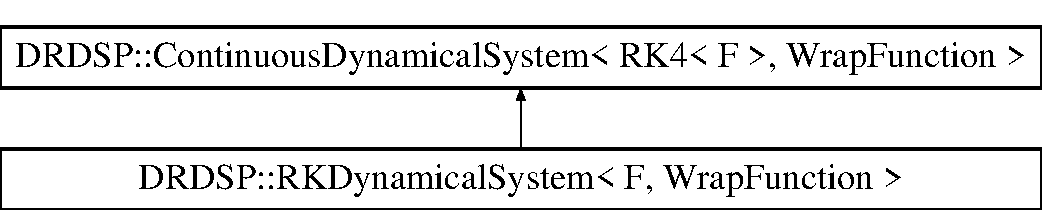
\includegraphics[height=2.000000cm]{struct_d_r_d_s_p_1_1_r_k_dynamical_system}
\end{center}
\end{figure}
\subsection*{Public Member Functions}
\begin{DoxyCompactItemize}
\item 
\hypertarget{struct_d_r_d_s_p_1_1_r_k_dynamical_system_ac4fddbaa65ce84accc167fc446fcfac7}{{\bfseries R\-K\-Dynamical\-System} (const F \&f)}\label{struct_d_r_d_s_p_1_1_r_k_dynamical_system_ac4fddbaa65ce84accc167fc446fcfac7}

\end{DoxyCompactItemize}
\subsection*{Additional Inherited Members}


The documentation for this struct was generated from the following file\-:\begin{DoxyCompactItemize}
\item 
include/\-D\-R\-D\-S\-P/dynamics/dynamical\-System.\-h\end{DoxyCompactItemize}

\hypertarget{struct_d_r_d_s_p_1_1_secants}{\section{D\-R\-D\-S\-P\-:\-:Secants Struct Reference}
\label{struct_d_r_d_s_p_1_1_secants}\index{D\-R\-D\-S\-P\-::\-Secants@{D\-R\-D\-S\-P\-::\-Secants}}
}
Inheritance diagram for D\-R\-D\-S\-P\-:\-:Secants\-:\begin{figure}[H]
\begin{center}
\leavevmode
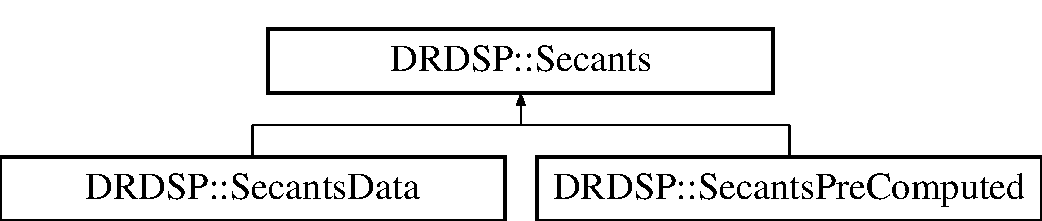
\includegraphics[height=2.000000cm]{struct_d_r_d_s_p_1_1_secants}
\end{center}
\end{figure}
\subsection*{Public Member Functions}
\begin{DoxyCompactItemize}
\item 
\hypertarget{struct_d_r_d_s_p_1_1_secants_a9fd886acfd2ffd083685f1c3a58db4fc}{virtual Vector\-Xd {\bfseries Get\-Secant} (uint32\-\_\-t k) const =0}\label{struct_d_r_d_s_p_1_1_secants_a9fd886acfd2ffd083685f1c3a58db4fc}

\item 
\hypertarget{struct_d_r_d_s_p_1_1_secants_a9b6763bc1541a775e842e437448200ef}{\hyperlink{struct_d_r_d_s_p_1_1_secants_pre_computed}{Secants\-Pre\-Computed} {\bfseries Cull\-Secants} (double tolerance) const }\label{struct_d_r_d_s_p_1_1_secants_a9b6763bc1541a775e842e437448200ef}

\item 
\hypertarget{struct_d_r_d_s_p_1_1_secants_abc02bf01e73c2d89848a090c88666291}{\hyperlink{struct_d_r_d_s_p_1_1_secants_pre_computed}{Secants\-Pre\-Computed} {\bfseries Cull\-Secants\-Degrees} (double degrees) const }\label{struct_d_r_d_s_p_1_1_secants_abc02bf01e73c2d89848a090c88666291}

\item 
\hypertarget{struct_d_r_d_s_p_1_1_secants_aec22fc746a9047366d7b81729a2e4f8a}{\hyperlink{struct_d_r_d_s_p_1_1_secants_pre_computed}{Secants\-Pre\-Computed} {\bfseries Cull\-Secants\-Radians} (double radians) const }\label{struct_d_r_d_s_p_1_1_secants_aec22fc746a9047366d7b81729a2e4f8a}

\end{DoxyCompactItemize}
\subsection*{Public Attributes}
\begin{DoxyCompactItemize}
\item 
\hypertarget{struct_d_r_d_s_p_1_1_secants_a0c6a707afa517ee01f1a2a76e1ed76bf}{uint32\-\_\-t {\bfseries count}}\label{struct_d_r_d_s_p_1_1_secants_a0c6a707afa517ee01f1a2a76e1ed76bf}

\item 
\hypertarget{struct_d_r_d_s_p_1_1_secants_a950d625f7d298f93eaad20062f79db1b}{uint32\-\_\-t {\bfseries dimension}}\label{struct_d_r_d_s_p_1_1_secants_a950d625f7d298f93eaad20062f79db1b}

\end{DoxyCompactItemize}


The documentation for this struct was generated from the following files\-:\begin{DoxyCompactItemize}
\item 
include/\-D\-R\-D\-S\-P/data/secants.\-h\item 
src/data/secants.\-cpp\end{DoxyCompactItemize}

\hypertarget{struct_d_r_d_s_p_1_1_secants_data}{\section{D\-R\-D\-S\-P\-:\-:Secants\-Data Struct Reference}
\label{struct_d_r_d_s_p_1_1_secants_data}\index{D\-R\-D\-S\-P\-::\-Secants\-Data@{D\-R\-D\-S\-P\-::\-Secants\-Data}}
}
Inheritance diagram for D\-R\-D\-S\-P\-:\-:Secants\-Data\-:\begin{figure}[H]
\begin{center}
\leavevmode
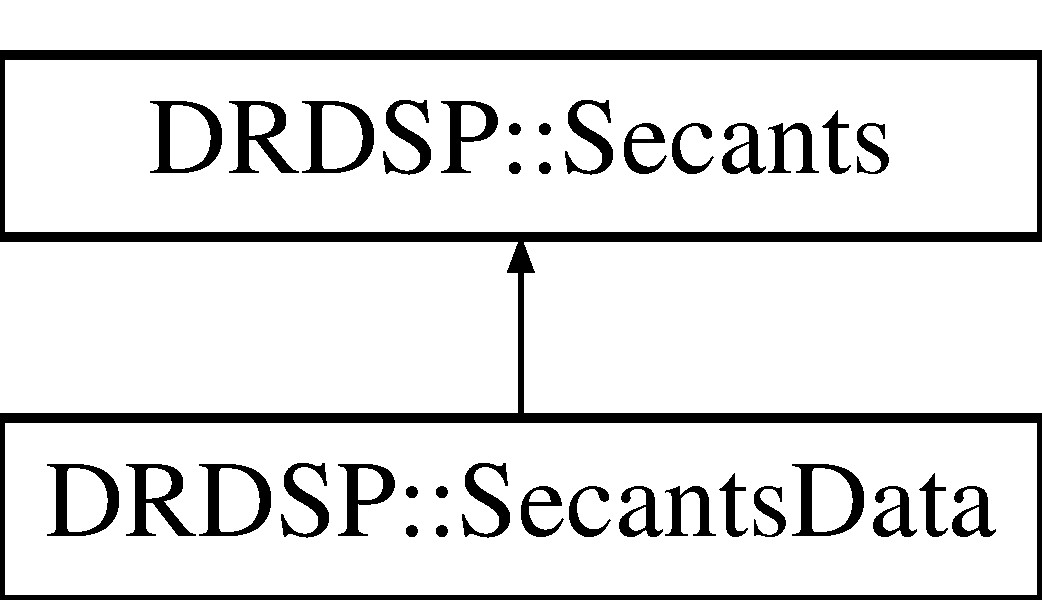
\includegraphics[height=2.000000cm]{struct_d_r_d_s_p_1_1_secants_data}
\end{center}
\end{figure}
\subsection*{Public Member Functions}
\begin{DoxyCompactItemize}
\item 
\hypertarget{struct_d_r_d_s_p_1_1_secants_data_a1c1383e3f4eca99473eba63d7a50a024}{void {\bfseries Set\-Data} (const \hyperlink{struct_d_r_d_s_p_1_1_data_set}{Data\-Set} \&data\-Set)}\label{struct_d_r_d_s_p_1_1_secants_data_a1c1383e3f4eca99473eba63d7a50a024}

\item 
\hypertarget{struct_d_r_d_s_p_1_1_secants_data_a7b94a05552fbbf08335ff1d4270ef13a}{Vector\-Xd {\bfseries Get\-Secant} (uint32\-\_\-t k) const }\label{struct_d_r_d_s_p_1_1_secants_data_a7b94a05552fbbf08335ff1d4270ef13a}

\end{DoxyCompactItemize}
\subsection*{Static Public Member Functions}
\begin{DoxyCompactItemize}
\item 
\hypertarget{struct_d_r_d_s_p_1_1_secants_data_abd9b205c7f0555f87195b241225e988b}{static uint32\-\_\-t {\bfseries Get\-Index\-I} (uint32\-\_\-t k, uint32\-\_\-t N)}\label{struct_d_r_d_s_p_1_1_secants_data_abd9b205c7f0555f87195b241225e988b}

\item 
\hypertarget{struct_d_r_d_s_p_1_1_secants_data_a7a609eef6b36cdd56d4920e312cc310e}{static uint32\-\_\-t {\bfseries Get\-Index\-J} (uint32\-\_\-t k, uint32\-\_\-t i, uint32\-\_\-t N)}\label{struct_d_r_d_s_p_1_1_secants_data_a7a609eef6b36cdd56d4920e312cc310e}

\end{DoxyCompactItemize}
\subsection*{Public Attributes}
\begin{DoxyCompactItemize}
\item 
\hypertarget{struct_d_r_d_s_p_1_1_secants_data_a1f2646fe6bfc11fdcf779344fc8d532c}{const \hyperlink{struct_d_r_d_s_p_1_1_data_set}{Data\-Set} $\ast$ {\bfseries data}}\label{struct_d_r_d_s_p_1_1_secants_data_a1f2646fe6bfc11fdcf779344fc8d532c}

\end{DoxyCompactItemize}


The documentation for this struct was generated from the following files\-:\begin{DoxyCompactItemize}
\item 
include/\-D\-R\-D\-S\-P/data/secants.\-h\item 
src/data/secants.\-cpp\end{DoxyCompactItemize}

\hypertarget{struct_d_r_d_s_p_1_1_secants_pre_computed}{\section{D\-R\-D\-S\-P\-:\-:Secants\-Pre\-Computed Struct Reference}
\label{struct_d_r_d_s_p_1_1_secants_pre_computed}\index{D\-R\-D\-S\-P\-::\-Secants\-Pre\-Computed@{D\-R\-D\-S\-P\-::\-Secants\-Pre\-Computed}}
}


Set of secants that have been pre-\/computed.  




{\ttfamily \#include $<$secants.\-h$>$}

Inheritance diagram for D\-R\-D\-S\-P\-:\-:Secants\-Pre\-Computed\-:\begin{figure}[H]
\begin{center}
\leavevmode
\includegraphics[height=2.000000cm]{struct_d_r_d_s_p_1_1_secants_pre_computed}
\end{center}
\end{figure}
\subsection*{Public Member Functions}
\begin{DoxyCompactItemize}
\item 
\hypertarget{struct_d_r_d_s_p_1_1_secants_pre_computed_a11e28de45102b068cf71cb2c9d6fca68}{{\bfseries Secants\-Pre\-Computed} (const \hyperlink{struct_d_r_d_s_p_1_1_secants_pre_computed}{Secants\-Pre\-Computed} \&rhs)}\label{struct_d_r_d_s_p_1_1_secants_pre_computed_a11e28de45102b068cf71cb2c9d6fca68}

\item 
\hypertarget{struct_d_r_d_s_p_1_1_secants_pre_computed_a9a23b0c9136fe8990a00be33787cb0f5}{{\bfseries Secants\-Pre\-Computed} (\hyperlink{struct_d_r_d_s_p_1_1_secants_pre_computed}{Secants\-Pre\-Computed} \&\&rhs)}\label{struct_d_r_d_s_p_1_1_secants_pre_computed_a9a23b0c9136fe8990a00be33787cb0f5}

\item 
\hypertarget{struct_d_r_d_s_p_1_1_secants_pre_computed_a7ca923d368f7131f8628eaf2bcf0d715}{\hyperlink{struct_d_r_d_s_p_1_1_secants_pre_computed}{Secants\-Pre\-Computed} \& {\bfseries operator=} (const \hyperlink{struct_d_r_d_s_p_1_1_secants_pre_computed}{Secants\-Pre\-Computed} \&rhs)}\label{struct_d_r_d_s_p_1_1_secants_pre_computed_a7ca923d368f7131f8628eaf2bcf0d715}

\item 
\hypertarget{struct_d_r_d_s_p_1_1_secants_pre_computed_afd36138af8143a3daa493d988938e784}{\hyperlink{struct_d_r_d_s_p_1_1_secants_pre_computed}{Secants\-Pre\-Computed} \& {\bfseries operator=} (\hyperlink{struct_d_r_d_s_p_1_1_secants_pre_computed}{Secants\-Pre\-Computed} \&\&rhs)}\label{struct_d_r_d_s_p_1_1_secants_pre_computed_afd36138af8143a3daa493d988938e784}

\item 
\hypertarget{struct_d_r_d_s_p_1_1_secants_pre_computed_a07644fb406546e3e6f5adbebd472a968}{void \hyperlink{struct_d_r_d_s_p_1_1_secants_pre_computed_a07644fb406546e3e6f5adbebd472a968}{Compute\-From\-Data} (const \hyperlink{struct_d_r_d_s_p_1_1_data_set}{Data\-Set} \&data\-Set)}\label{struct_d_r_d_s_p_1_1_secants_pre_computed_a07644fb406546e3e6f5adbebd472a968}

\begin{DoxyCompactList}\small\item\em Compute this set of secants from the given data set. \end{DoxyCompactList}\item 
\hypertarget{struct_d_r_d_s_p_1_1_secants_pre_computed_a6b9de4610d5af4f02ab7b0c6fc326ed8}{Vector\-Xd \hyperlink{struct_d_r_d_s_p_1_1_secants_pre_computed_a6b9de4610d5af4f02ab7b0c6fc326ed8}{Get\-Secant} (uint32\-\_\-t k) const }\label{struct_d_r_d_s_p_1_1_secants_pre_computed_a6b9de4610d5af4f02ab7b0c6fc326ed8}

\begin{DoxyCompactList}\small\item\em Get the kth secant (normalized) \end{DoxyCompactList}\item 
\hypertarget{struct_d_r_d_s_p_1_1_secants_pre_computed_aedd413333624ec2b3da2a70262b65481}{Vector\-Xd \hyperlink{struct_d_r_d_s_p_1_1_secants_pre_computed_aedd413333624ec2b3da2a70262b65481}{Get\-Secant\-No\-Normalize} (uint32\-\_\-t k) const }\label{struct_d_r_d_s_p_1_1_secants_pre_computed_aedd413333624ec2b3da2a70262b65481}

\begin{DoxyCompactList}\small\item\em Get the kth secant (not necessarily normalized) \end{DoxyCompactList}\item 
\hypertarget{struct_d_r_d_s_p_1_1_secants_pre_computed_a8dcdb9edcefeee50e17d6ab3b792f5e6}{\hyperlink{struct_d_r_d_s_p_1_1_secants_pre_computed}{Secants\-Pre\-Computed} {\bfseries Cull\-Secants} (double tolerance) const }\label{struct_d_r_d_s_p_1_1_secants_pre_computed_a8dcdb9edcefeee50e17d6ab3b792f5e6}

\end{DoxyCompactItemize}
\subsection*{Public Attributes}
\begin{DoxyCompactItemize}
\item 
\hypertarget{struct_d_r_d_s_p_1_1_secants_pre_computed_a15231ffddb89ae1eb2c83cbdc463905a}{Vector\-Xd $\ast$ \hyperlink{struct_d_r_d_s_p_1_1_secants_pre_computed_a15231ffddb89ae1eb2c83cbdc463905a}{secants}}\label{struct_d_r_d_s_p_1_1_secants_pre_computed_a15231ffddb89ae1eb2c83cbdc463905a}

\begin{DoxyCompactList}\small\item\em Array of pre-\/computed unit secants. \end{DoxyCompactList}\item 
\hypertarget{struct_d_r_d_s_p_1_1_secants_pre_computed_a4bb39354f325540fefe37eb7c3f59ad1}{weight\-Type $\ast$ \hyperlink{struct_d_r_d_s_p_1_1_secants_pre_computed_a4bb39354f325540fefe37eb7c3f59ad1}{weights}}\label{struct_d_r_d_s_p_1_1_secants_pre_computed_a4bb39354f325540fefe37eb7c3f59ad1}

\begin{DoxyCompactList}\small\item\em Array of secant weights produced by culling. \end{DoxyCompactList}\end{DoxyCompactItemize}


\subsection{Detailed Description}
Set of secants that have been pre-\/computed. 

The documentation for this struct was generated from the following files\-:\begin{DoxyCompactItemize}
\item 
include/\-D\-R\-D\-S\-P/data/secants.\-h\item 
src/data/secants.\-cpp\end{DoxyCompactItemize}

\hypertarget{struct_d_r_d_s_p_1_1_secants_system}{\section{D\-R\-D\-S\-P\-:\-:Secants\-System Struct Reference}
\label{struct_d_r_d_s_p_1_1_secants_system}\index{D\-R\-D\-S\-P\-::\-Secants\-System@{D\-R\-D\-S\-P\-::\-Secants\-System}}
}
\subsection*{Public Attributes}
\begin{DoxyCompactItemize}
\item 
\hypertarget{struct_d_r_d_s_p_1_1_secants_system_a9c69d703c71a37c58cf9202ef8726336}{const \hyperlink{struct_d_r_d_s_p_1_1_secants_pre_computed}{Secants\-Pre\-Computed} $\ast$ {\bfseries secants}}\label{struct_d_r_d_s_p_1_1_secants_system_a9c69d703c71a37c58cf9202ef8726336}

\item 
\hypertarget{struct_d_r_d_s_p_1_1_secants_system_ac656492eccbaef7e14330fdacfbecdb2}{uint16\-\_\-t {\bfseries N}}\label{struct_d_r_d_s_p_1_1_secants_system_ac656492eccbaef7e14330fdacfbecdb2}

\end{DoxyCompactItemize}


The documentation for this struct was generated from the following file\-:\begin{DoxyCompactItemize}
\item 
include/\-D\-R\-D\-S\-P/projection/proj\-\_\-secant.\-h\end{DoxyCompactItemize}

\hypertarget{struct_d_r_d_s_p_1_1_solver}{\section{D\-R\-D\-S\-P\-:\-:Solver$<$ T\-Time, T\-State $>$ Struct Template Reference}
\label{struct_d_r_d_s_p_1_1_solver}\index{D\-R\-D\-S\-P\-::\-Solver$<$ T\-Time, T\-State $>$@{D\-R\-D\-S\-P\-::\-Solver$<$ T\-Time, T\-State $>$}}
}
Inheritance diagram for D\-R\-D\-S\-P\-:\-:Solver$<$ T\-Time, T\-State $>$\-:\begin{figure}[H]
\begin{center}
\leavevmode
\includegraphics[height=2.000000cm]{struct_d_r_d_s_p_1_1_solver}
\end{center}
\end{figure}
\subsection*{Public Member Functions}
\begin{DoxyCompactItemize}
\item 
\hypertarget{struct_d_r_d_s_p_1_1_solver_a0e90b6f21779b243987578e2a5c9907a}{{\bfseries Solver} (\hyperlink{struct_d_r_d_s_p_1_1_solver_function}{Solver\-Function}$<$ T\-Time, T\-State $>$ \&f)}\label{struct_d_r_d_s_p_1_1_solver_a0e90b6f21779b243987578e2a5c9907a}

\item 
\hypertarget{struct_d_r_d_s_p_1_1_solver_ac92dbb47d907f32153deb365990b7f89}{virtual void {\bfseries Integrate} (T\-State \&x, T\-Time \&t, T\-Time dt)=0}\label{struct_d_r_d_s_p_1_1_solver_ac92dbb47d907f32153deb365990b7f89}

\end{DoxyCompactItemize}
\subsection*{Public Attributes}
\begin{DoxyCompactItemize}
\item 
\hypertarget{struct_d_r_d_s_p_1_1_solver_ab0322a69134c46c56debe861f8b1f98f}{\hyperlink{struct_d_r_d_s_p_1_1_solver_function}{Solver\-Function}$<$ T\-Time, T\-State $>$ \& {\bfseries Function}}\label{struct_d_r_d_s_p_1_1_solver_ab0322a69134c46c56debe861f8b1f98f}

\end{DoxyCompactItemize}


The documentation for this struct was generated from the following file\-:\begin{DoxyCompactItemize}
\item 
include/\-D\-R\-D\-S\-P/dynamics/solver.\-h\end{DoxyCompactItemize}

\hypertarget{struct_d_r_d_s_p_1_1_solver_function}{\section{D\-R\-D\-S\-P\-:\-:Solver\-Function$<$ T\-Time, T\-State $>$ Struct Template Reference}
\label{struct_d_r_d_s_p_1_1_solver_function}\index{D\-R\-D\-S\-P\-::\-Solver\-Function$<$ T\-Time, T\-State $>$@{D\-R\-D\-S\-P\-::\-Solver\-Function$<$ T\-Time, T\-State $>$}}
}
\subsection*{Public Member Functions}
\begin{DoxyCompactItemize}
\item 
\hypertarget{struct_d_r_d_s_p_1_1_solver_function_a4ced40af4a699021bc38a121e65babb5}{virtual T\-State {\bfseries operator()} (const T\-State \&x, T\-Time t)=0}\label{struct_d_r_d_s_p_1_1_solver_function_a4ced40af4a699021bc38a121e65babb5}

\end{DoxyCompactItemize}


The documentation for this struct was generated from the following file\-:\begin{DoxyCompactItemize}
\item 
include/\-D\-R\-D\-S\-P/dynamics/solver.\-h\end{DoxyCompactItemize}

\hypertarget{struct_d_r_d_s_p_1_1_thin_plate_spline}{\section{D\-R\-D\-S\-P\-:\-:Thin\-Plate\-Spline Struct Reference}
\label{struct_d_r_d_s_p_1_1_thin_plate_spline}\index{D\-R\-D\-S\-P\-::\-Thin\-Plate\-Spline@{D\-R\-D\-S\-P\-::\-Thin\-Plate\-Spline}}
}
Inheritance diagram for D\-R\-D\-S\-P\-:\-:Thin\-Plate\-Spline\-:\begin{figure}[H]
\begin{center}
\leavevmode
\includegraphics[height=2.000000cm]{struct_d_r_d_s_p_1_1_thin_plate_spline}
\end{center}
\end{figure}
\subsection*{Public Member Functions}
\begin{DoxyCompactItemize}
\item 
\hypertarget{struct_d_r_d_s_p_1_1_thin_plate_spline_a0282d868aa5e4f4cb077ed61dd343a0a}{double {\bfseries operator()} (double r) const }\label{struct_d_r_d_s_p_1_1_thin_plate_spline_a0282d868aa5e4f4cb077ed61dd343a0a}

\item 
\hypertarget{struct_d_r_d_s_p_1_1_thin_plate_spline_a42377bcfa0b624e7dc2569a411d06b19}{double {\bfseries Derivative} (double r) const }\label{struct_d_r_d_s_p_1_1_thin_plate_spline_a42377bcfa0b624e7dc2569a411d06b19}

\end{DoxyCompactItemize}


The documentation for this struct was generated from the following files\-:\begin{DoxyCompactItemize}
\item 
include/\-D\-R\-D\-S\-P/dynamics/radial\-\_\-basis.\-h\item 
src/dynamics/radial\-\_\-basis.\-cpp\end{DoxyCompactItemize}

\hypertarget{struct_d_r_d_s_p_1_1_traits}{\section{D\-R\-D\-S\-P\-:\-:Traits$<$ V $>$ Struct Template Reference}
\label{struct_d_r_d_s_p_1_1_traits}\index{D\-R\-D\-S\-P\-::\-Traits$<$ V $>$@{D\-R\-D\-S\-P\-::\-Traits$<$ V $>$}}
}


The documentation for this struct was generated from the following file\-:\begin{DoxyCompactItemize}
\item 
include/\-D\-R\-D\-S\-P/geometry/geodesic.\-h\end{DoxyCompactItemize}

\hypertarget{struct_d_r_d_s_p_1_1_traits_3_01double_01_4}{\section{D\-R\-D\-S\-P\-:\-:Traits$<$ double $>$ Struct Template Reference}
\label{struct_d_r_d_s_p_1_1_traits_3_01double_01_4}\index{D\-R\-D\-S\-P\-::\-Traits$<$ double $>$@{D\-R\-D\-S\-P\-::\-Traits$<$ double $>$}}
}
\subsection*{Public Types}
\begin{DoxyCompactItemize}
\item 
\hypertarget{struct_d_r_d_s_p_1_1_traits_3_01double_01_4_a7ca4b622dcdefa389bfbae5ba70f6467}{typedef double {\bfseries T\-Scalar}}\label{struct_d_r_d_s_p_1_1_traits_3_01double_01_4_a7ca4b622dcdefa389bfbae5ba70f6467}

\end{DoxyCompactItemize}


The documentation for this struct was generated from the following file\-:\begin{DoxyCompactItemize}
\item 
include/\-D\-R\-D\-S\-P/geometry/vector.\-h\end{DoxyCompactItemize}

\hypertarget{struct_d_r_d_s_p_1_1_traits_3_01float_01_4}{\section{D\-R\-D\-S\-P\-:\-:Traits$<$ float $>$ Struct Template Reference}
\label{struct_d_r_d_s_p_1_1_traits_3_01float_01_4}\index{D\-R\-D\-S\-P\-::\-Traits$<$ float $>$@{D\-R\-D\-S\-P\-::\-Traits$<$ float $>$}}
}
\subsection*{Public Types}
\begin{DoxyCompactItemize}
\item 
\hypertarget{struct_d_r_d_s_p_1_1_traits_3_01float_01_4_a743d312f54b9ce220bf37be4f12a5b6a}{typedef float {\bfseries T\-Scalar}}\label{struct_d_r_d_s_p_1_1_traits_3_01float_01_4_a743d312f54b9ce220bf37be4f12a5b6a}

\end{DoxyCompactItemize}


The documentation for this struct was generated from the following file\-:\begin{DoxyCompactItemize}
\item 
include/\-D\-R\-D\-S\-P/geometry/vector.\-h\end{DoxyCompactItemize}

\hypertarget{struct_d_r_d_s_p_1_1_traits_3_01_matrix_3_01___scalar_00_01___rows_00_01___cols_00_01___options_7f94984544c1bbd2d14e661033a6db2c}{\section{D\-R\-D\-S\-P\-:\-:Traits$<$ Matrix$<$ \-\_\-\-Scalar, \-\_\-\-Rows, \-\_\-\-Cols, \-\_\-\-Options, \-\_\-\-Max\-Rows, \-\_\-\-Max\-Cols $>$ $>$ Struct Template Reference}
\label{struct_d_r_d_s_p_1_1_traits_3_01_matrix_3_01___scalar_00_01___rows_00_01___cols_00_01___options_7f94984544c1bbd2d14e661033a6db2c}\index{D\-R\-D\-S\-P\-::\-Traits$<$ Matrix$<$ \-\_\-\-Scalar, \-\_\-\-Rows, \-\_\-\-Cols, \-\_\-\-Options, \-\_\-\-Max\-Rows, \-\_\-\-Max\-Cols $>$ $>$@{D\-R\-D\-S\-P\-::\-Traits$<$ Matrix$<$ \-\_\-\-Scalar, \-\_\-\-Rows, \-\_\-\-Cols, \-\_\-\-Options, \-\_\-\-Max\-Rows, \-\_\-\-Max\-Cols $>$ $>$}}
}
\subsection*{Public Types}
\begin{DoxyCompactItemize}
\item 
\hypertarget{struct_d_r_d_s_p_1_1_traits_3_01_matrix_3_01___scalar_00_01___rows_00_01___cols_00_01___options_7f94984544c1bbd2d14e661033a6db2c_afafc8db9b7ec6e18a81aa0b25cd2f729}{typedef Matrix$<$ \-\_\-\-Scalar, \-\_\-\-Rows, \\*
\-\_\-\-Cols, \-\_\-\-Options, \-\_\-\-Max\-Rows, \\*
\-\_\-\-Max\-Cols $>$\-::Scalar {\bfseries T\-Scalar}}\label{struct_d_r_d_s_p_1_1_traits_3_01_matrix_3_01___scalar_00_01___rows_00_01___cols_00_01___options_7f94984544c1bbd2d14e661033a6db2c_afafc8db9b7ec6e18a81aa0b25cd2f729}

\end{DoxyCompactItemize}


The documentation for this struct was generated from the following file\-:\begin{DoxyCompactItemize}
\item 
include/\-D\-R\-D\-S\-P/geometry/vector.\-h\end{DoxyCompactItemize}

\hypertarget{struct_d_r_d_s_p_1_1_traits_3_01_metric_uniform_3_01___t_i_p_01_4_01_4}{\section{D\-R\-D\-S\-P\-:\-:Traits$<$ Metric\-Uniform$<$ \-\_\-\-T\-I\-P $>$ $>$ Struct Template Reference}
\label{struct_d_r_d_s_p_1_1_traits_3_01_metric_uniform_3_01___t_i_p_01_4_01_4}\index{D\-R\-D\-S\-P\-::\-Traits$<$ Metric\-Uniform$<$ \-\_\-\-T\-I\-P $>$ $>$@{D\-R\-D\-S\-P\-::\-Traits$<$ Metric\-Uniform$<$ \-\_\-\-T\-I\-P $>$ $>$}}
}
\subsection*{Public Types}
\begin{DoxyCompactItemize}
\item 
\hypertarget{struct_d_r_d_s_p_1_1_traits_3_01_metric_uniform_3_01___t_i_p_01_4_01_4_a2e0cc0577541aa569740718f52f9902e}{typedef \-\_\-\-T\-I\-P {\bfseries T\-I\-P}}\label{struct_d_r_d_s_p_1_1_traits_3_01_metric_uniform_3_01___t_i_p_01_4_01_4_a2e0cc0577541aa569740718f52f9902e}

\item 
\hypertarget{struct_d_r_d_s_p_1_1_traits_3_01_metric_uniform_3_01___t_i_p_01_4_01_4_a5cd7d42a3d2518fb97d0c1afe74e5941}{typedef \hyperlink{struct_d_r_d_s_p_1_1_traits}{Traits}$<$ T\-I\-P $>$\-::T\-C\-V {\bfseries T\-C\-V}}\label{struct_d_r_d_s_p_1_1_traits_3_01_metric_uniform_3_01___t_i_p_01_4_01_4_a5cd7d42a3d2518fb97d0c1afe74e5941}

\item 
\hypertarget{struct_d_r_d_s_p_1_1_traits_3_01_metric_uniform_3_01___t_i_p_01_4_01_4_afba860f2dd7a97e53162db743b4acebd}{typedef \hyperlink{struct_d_r_d_s_p_1_1_traits}{Traits}$<$ T\-I\-P $>$\-::T\-Vec {\bfseries T\-Vec}}\label{struct_d_r_d_s_p_1_1_traits_3_01_metric_uniform_3_01___t_i_p_01_4_01_4_afba860f2dd7a97e53162db743b4acebd}

\item 
\hypertarget{struct_d_r_d_s_p_1_1_traits_3_01_metric_uniform_3_01___t_i_p_01_4_01_4_a392deed657c6716f92e17e4d541a6826}{typedef \hyperlink{struct_d_r_d_s_p_1_1_traits}{Traits}$<$ T\-I\-P $>$\-::T\-Scalar {\bfseries T\-Scalar}}\label{struct_d_r_d_s_p_1_1_traits_3_01_metric_uniform_3_01___t_i_p_01_4_01_4_a392deed657c6716f92e17e4d541a6826}

\end{DoxyCompactItemize}


The documentation for this struct was generated from the following file\-:\begin{DoxyCompactItemize}
\item 
include/\-D\-R\-D\-S\-P/geometry/metric.\-h\end{DoxyCompactItemize}

\hypertarget{struct_d_r_d_s_p_1_1_traits_3_01struct_01_co_matrix_xd_01_4}{\section{D\-R\-D\-S\-P\-:\-:Traits$<$ struct Co\-Matrix\-Xd $>$ Struct Template Reference}
\label{struct_d_r_d_s_p_1_1_traits_3_01struct_01_co_matrix_xd_01_4}\index{D\-R\-D\-S\-P\-::\-Traits$<$ struct Co\-Matrix\-Xd $>$@{D\-R\-D\-S\-P\-::\-Traits$<$ struct Co\-Matrix\-Xd $>$}}
}
\subsection*{Public Types}
\begin{DoxyCompactItemize}
\item 
\hypertarget{struct_d_r_d_s_p_1_1_traits_3_01struct_01_co_matrix_xd_01_4_a6702092e83b4ea57cdaa6ab3ba3c9819}{typedef Matrix\-Xd {\bfseries T\-Vec}}\label{struct_d_r_d_s_p_1_1_traits_3_01struct_01_co_matrix_xd_01_4_a6702092e83b4ea57cdaa6ab3ba3c9819}

\item 
\hypertarget{struct_d_r_d_s_p_1_1_traits_3_01struct_01_co_matrix_xd_01_4_ac5c1214e7dbb6927ad7edccb2e5ee12f}{typedef \hyperlink{struct_d_r_d_s_p_1_1_traits}{Traits}$<$ T\-Vec $>$\-::T\-Scalar {\bfseries T\-Scalar}}\label{struct_d_r_d_s_p_1_1_traits_3_01struct_01_co_matrix_xd_01_4_ac5c1214e7dbb6927ad7edccb2e5ee12f}

\end{DoxyCompactItemize}


The documentation for this struct was generated from the following file\-:\begin{DoxyCompactItemize}
\item 
include/\-D\-R\-D\-S\-P/geometry/vector.\-h\end{DoxyCompactItemize}

\hypertarget{struct_d_r_d_s_p_1_1_traits_3_01struct_01_co_vector_xd_01_4}{\section{D\-R\-D\-S\-P\-:\-:Traits$<$ struct Co\-Vector\-Xd $>$ Struct Template Reference}
\label{struct_d_r_d_s_p_1_1_traits_3_01struct_01_co_vector_xd_01_4}\index{D\-R\-D\-S\-P\-::\-Traits$<$ struct Co\-Vector\-Xd $>$@{D\-R\-D\-S\-P\-::\-Traits$<$ struct Co\-Vector\-Xd $>$}}
}
\subsection*{Public Types}
\begin{DoxyCompactItemize}
\item 
\hypertarget{struct_d_r_d_s_p_1_1_traits_3_01struct_01_co_vector_xd_01_4_aebf9a61ca9132aadba80b889a3e3e8c3}{typedef Vector\-Xd {\bfseries T\-Vec}}\label{struct_d_r_d_s_p_1_1_traits_3_01struct_01_co_vector_xd_01_4_aebf9a61ca9132aadba80b889a3e3e8c3}

\item 
\hypertarget{struct_d_r_d_s_p_1_1_traits_3_01struct_01_co_vector_xd_01_4_a399aec522527420dc77ba3fd95bdbf76}{typedef \hyperlink{struct_d_r_d_s_p_1_1_traits}{Traits}$<$ T\-Vec $>$\-::T\-Scalar {\bfseries T\-Scalar}}\label{struct_d_r_d_s_p_1_1_traits_3_01struct_01_co_vector_xd_01_4_a399aec522527420dc77ba3fd95bdbf76}

\end{DoxyCompactItemize}


The documentation for this struct was generated from the following file\-:\begin{DoxyCompactItemize}
\item 
include/\-D\-R\-D\-S\-P/geometry/vector.\-h\end{DoxyCompactItemize}

\hypertarget{struct_d_r_d_s_p_1_1_traits_3_01struct_01_i_p_dot_01_4}{\section{D\-R\-D\-S\-P\-:\-:Traits$<$ struct I\-P\-Dot $>$ Struct Template Reference}
\label{struct_d_r_d_s_p_1_1_traits_3_01struct_01_i_p_dot_01_4}\index{D\-R\-D\-S\-P\-::\-Traits$<$ struct I\-P\-Dot $>$@{D\-R\-D\-S\-P\-::\-Traits$<$ struct I\-P\-Dot $>$}}
}
\subsection*{Public Types}
\begin{DoxyCompactItemize}
\item 
\hypertarget{struct_d_r_d_s_p_1_1_traits_3_01struct_01_i_p_dot_01_4_aa9077bf7b2e5fd9130525e4442082f49}{typedef \hyperlink{struct_d_r_d_s_p_1_1_co_vector_xd}{Co\-Vector\-Xd} {\bfseries T\-C\-V}}\label{struct_d_r_d_s_p_1_1_traits_3_01struct_01_i_p_dot_01_4_aa9077bf7b2e5fd9130525e4442082f49}

\item 
\hypertarget{struct_d_r_d_s_p_1_1_traits_3_01struct_01_i_p_dot_01_4_a2c2052b4655b41dd1ad57407be283524}{typedef \hyperlink{struct_d_r_d_s_p_1_1_traits}{Traits}$<$ \hyperlink{struct_d_r_d_s_p_1_1_co_vector_xd}{T\-C\-V} $>$\-::T\-Vec {\bfseries T\-Vec}}\label{struct_d_r_d_s_p_1_1_traits_3_01struct_01_i_p_dot_01_4_a2c2052b4655b41dd1ad57407be283524}

\item 
\hypertarget{struct_d_r_d_s_p_1_1_traits_3_01struct_01_i_p_dot_01_4_a4079bbff8395a69eefb9352209db8227}{typedef \hyperlink{struct_d_r_d_s_p_1_1_traits}{Traits}$<$ T\-Vec $>$\-::T\-Scalar {\bfseries T\-Scalar}}\label{struct_d_r_d_s_p_1_1_traits_3_01struct_01_i_p_dot_01_4_a4079bbff8395a69eefb9352209db8227}

\end{DoxyCompactItemize}


The documentation for this struct was generated from the following file\-:\begin{DoxyCompactItemize}
\item 
include/\-D\-R\-D\-S\-P/geometry/inner\-\_\-product.\-h\end{DoxyCompactItemize}

\hypertarget{struct_d_r_d_s_p_1_1_traits_3_01struct_01_i_p_frobenius_01_4}{\section{D\-R\-D\-S\-P\-:\-:Traits$<$ struct I\-P\-Frobenius $>$ Struct Template Reference}
\label{struct_d_r_d_s_p_1_1_traits_3_01struct_01_i_p_frobenius_01_4}\index{D\-R\-D\-S\-P\-::\-Traits$<$ struct I\-P\-Frobenius $>$@{D\-R\-D\-S\-P\-::\-Traits$<$ struct I\-P\-Frobenius $>$}}
}
\subsection*{Public Types}
\begin{DoxyCompactItemize}
\item 
\hypertarget{struct_d_r_d_s_p_1_1_traits_3_01struct_01_i_p_frobenius_01_4_aa2dc7d64d9cb681fa92250cbb1dc81c2}{typedef \hyperlink{struct_d_r_d_s_p_1_1_co_matrix_xd}{Co\-Matrix\-Xd} {\bfseries T\-C\-V}}\label{struct_d_r_d_s_p_1_1_traits_3_01struct_01_i_p_frobenius_01_4_aa2dc7d64d9cb681fa92250cbb1dc81c2}

\item 
\hypertarget{struct_d_r_d_s_p_1_1_traits_3_01struct_01_i_p_frobenius_01_4_a406d1575c5f00fa20c68393270f154b8}{typedef \hyperlink{struct_d_r_d_s_p_1_1_traits}{Traits}$<$ \hyperlink{struct_d_r_d_s_p_1_1_co_matrix_xd}{T\-C\-V} $>$\-::T\-Vec {\bfseries T\-Vec}}\label{struct_d_r_d_s_p_1_1_traits_3_01struct_01_i_p_frobenius_01_4_a406d1575c5f00fa20c68393270f154b8}

\item 
\hypertarget{struct_d_r_d_s_p_1_1_traits_3_01struct_01_i_p_frobenius_01_4_a745fb704d12a2e95ba4c24b359e765e9}{typedef \hyperlink{struct_d_r_d_s_p_1_1_traits}{Traits}$<$ T\-Vec $>$\-::T\-Scalar {\bfseries T\-Scalar}}\label{struct_d_r_d_s_p_1_1_traits_3_01struct_01_i_p_frobenius_01_4_a745fb704d12a2e95ba4c24b359e765e9}

\end{DoxyCompactItemize}


The documentation for this struct was generated from the following file\-:\begin{DoxyCompactItemize}
\item 
include/\-D\-R\-D\-S\-P/geometry/inner\-\_\-product.\-h\end{DoxyCompactItemize}

\hypertarget{struct_d_r_d_s_p_1_1_traits_3_01struct_01_i_p_vector_01_4}{\section{D\-R\-D\-S\-P\-:\-:Traits$<$ struct I\-P\-Vector $>$ Struct Template Reference}
\label{struct_d_r_d_s_p_1_1_traits_3_01struct_01_i_p_vector_01_4}\index{D\-R\-D\-S\-P\-::\-Traits$<$ struct I\-P\-Vector $>$@{D\-R\-D\-S\-P\-::\-Traits$<$ struct I\-P\-Vector $>$}}
}
\subsection*{Public Types}
\begin{DoxyCompactItemize}
\item 
\hypertarget{struct_d_r_d_s_p_1_1_traits_3_01struct_01_i_p_vector_01_4_a4cd9c5279190cc8725fef7bc66830a5e}{typedef \hyperlink{struct_d_r_d_s_p_1_1_co_vector_xd}{Co\-Vector\-Xd} {\bfseries T\-C\-V}}\label{struct_d_r_d_s_p_1_1_traits_3_01struct_01_i_p_vector_01_4_a4cd9c5279190cc8725fef7bc66830a5e}

\item 
\hypertarget{struct_d_r_d_s_p_1_1_traits_3_01struct_01_i_p_vector_01_4_a4eba2a5c184d06a8f7e06ae6fe2f2664}{typedef \hyperlink{struct_d_r_d_s_p_1_1_traits}{Traits}$<$ \hyperlink{struct_d_r_d_s_p_1_1_co_vector_xd}{T\-C\-V} $>$\-::T\-Vec {\bfseries T\-Vec}}\label{struct_d_r_d_s_p_1_1_traits_3_01struct_01_i_p_vector_01_4_a4eba2a5c184d06a8f7e06ae6fe2f2664}

\item 
\hypertarget{struct_d_r_d_s_p_1_1_traits_3_01struct_01_i_p_vector_01_4_a3c954ce780dd48092a7bada2aaae8c89}{typedef \hyperlink{struct_d_r_d_s_p_1_1_traits}{Traits}$<$ T\-Vec $>$\-::T\-Scalar {\bfseries T\-Scalar}}\label{struct_d_r_d_s_p_1_1_traits_3_01struct_01_i_p_vector_01_4_a3c954ce780dd48092a7bada2aaae8c89}

\end{DoxyCompactItemize}


The documentation for this struct was generated from the following file\-:\begin{DoxyCompactItemize}
\item 
include/\-D\-R\-D\-S\-P/geometry/inner\-\_\-product.\-h\end{DoxyCompactItemize}

\hypertarget{struct_d_r_d_s_p_1_1_vector}{\section{D\-R\-D\-S\-P\-:\-:Vector$<$ Derived $>$ Struct Template Reference}
\label{struct_d_r_d_s_p_1_1_vector}\index{D\-R\-D\-S\-P\-::\-Vector$<$ Derived $>$@{D\-R\-D\-S\-P\-::\-Vector$<$ Derived $>$}}
}
Inheritance diagram for D\-R\-D\-S\-P\-:\-:Vector$<$ Derived $>$\-:\begin{figure}[H]
\begin{center}
\leavevmode
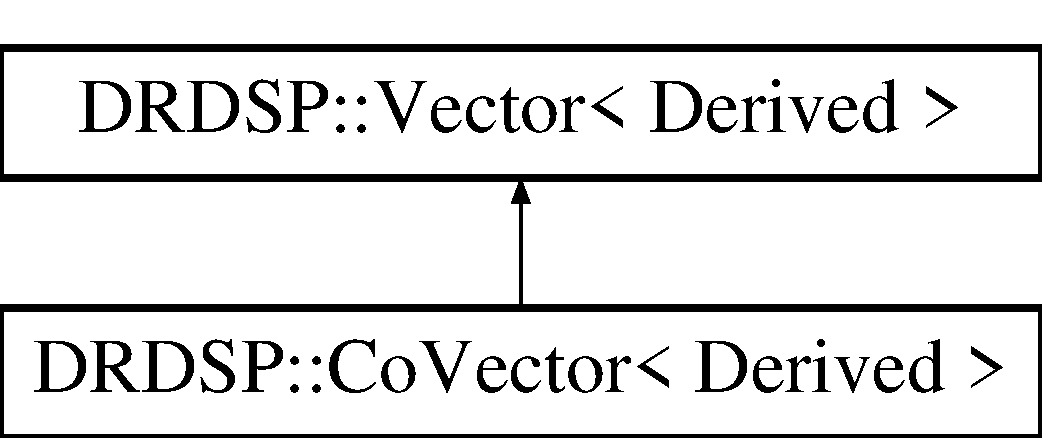
\includegraphics[height=2.000000cm]{struct_d_r_d_s_p_1_1_vector}
\end{center}
\end{figure}
\subsection*{Public Types}
\begin{DoxyCompactItemize}
\item 
\hypertarget{struct_d_r_d_s_p_1_1_vector_a579b48d72ce51c48a98e8bdd1d009782}{typedef \hyperlink{struct_d_r_d_s_p_1_1_traits}{Traits}$<$ Derived $>$\-::T\-Scalar {\bfseries T\-Scalar}}\label{struct_d_r_d_s_p_1_1_vector_a579b48d72ce51c48a98e8bdd1d009782}

\end{DoxyCompactItemize}
\subsection*{Public Member Functions}
\begin{DoxyCompactItemize}
\item 
\hypertarget{struct_d_r_d_s_p_1_1_vector_ae0414720f2f7df0f93db48ec06a5bffa}{virtual Derived {\bfseries operator+} (const Derived \&V) const =0}\label{struct_d_r_d_s_p_1_1_vector_ae0414720f2f7df0f93db48ec06a5bffa}

\item 
\hypertarget{struct_d_r_d_s_p_1_1_vector_af834765f99b0fb9bc831232130e65e9a}{virtual Derived \& {\bfseries operator+=} (const Derived \&V)=0}\label{struct_d_r_d_s_p_1_1_vector_af834765f99b0fb9bc831232130e65e9a}

\item 
\hypertarget{struct_d_r_d_s_p_1_1_vector_a8420652d7d12d600cfdf8b93c2d097f7}{virtual Derived {\bfseries operator-\/} (const Derived \&V) const =0}\label{struct_d_r_d_s_p_1_1_vector_a8420652d7d12d600cfdf8b93c2d097f7}

\item 
\hypertarget{struct_d_r_d_s_p_1_1_vector_afdbe13820fd8449fa9db2b5efdc6c63c}{virtual Derived \& {\bfseries operator-\/=} (const Derived \&V)=0}\label{struct_d_r_d_s_p_1_1_vector_afdbe13820fd8449fa9db2b5efdc6c63c}

\item 
\hypertarget{struct_d_r_d_s_p_1_1_vector_a18d15ba8f747ec0e8056aa009a755647}{virtual Derived {\bfseries operator$\ast$} (const T\-Scalar \&a) const =0}\label{struct_d_r_d_s_p_1_1_vector_a18d15ba8f747ec0e8056aa009a755647}

\item 
\hypertarget{struct_d_r_d_s_p_1_1_vector_a49fd2816abf9072c70f8f1ba99d596d2}{virtual Derived \& {\bfseries operator$\ast$=} (const T\-Scalar \&a)=0}\label{struct_d_r_d_s_p_1_1_vector_a49fd2816abf9072c70f8f1ba99d596d2}

\item 
\hypertarget{struct_d_r_d_s_p_1_1_vector_a8615194b57aad6762166047c28568175}{virtual Derived {\bfseries operator/} (const T\-Scalar \&a) const =0}\label{struct_d_r_d_s_p_1_1_vector_a8615194b57aad6762166047c28568175}

\item 
\hypertarget{struct_d_r_d_s_p_1_1_vector_af56f733484ef09cef2f7c439f754e636}{virtual Derived \& {\bfseries operator/=} (const T\-Scalar \&a)=0}\label{struct_d_r_d_s_p_1_1_vector_af56f733484ef09cef2f7c439f754e636}

\item 
\hypertarget{struct_d_r_d_s_p_1_1_vector_a237f4841398cd0822f2438b390864ee6}{virtual Derived {\bfseries operator-\/} () const =0}\label{struct_d_r_d_s_p_1_1_vector_a237f4841398cd0822f2438b390864ee6}

\end{DoxyCompactItemize}


The documentation for this struct was generated from the following file\-:\begin{DoxyCompactItemize}
\item 
include/\-D\-R\-D\-S\-P/geometry/vector.\-h\end{DoxyCompactItemize}

\hypertarget{struct_d_r_d_s_p_1_1_wrap_function}{\section{D\-R\-D\-S\-P\-:\-:Wrap\-Function$<$ T\-State $>$ Struct Template Reference}
\label{struct_d_r_d_s_p_1_1_wrap_function}\index{D\-R\-D\-S\-P\-::\-Wrap\-Function$<$ T\-State $>$@{D\-R\-D\-S\-P\-::\-Wrap\-Function$<$ T\-State $>$}}
}
\subsection*{Public Member Functions}
\begin{DoxyCompactItemize}
\item 
\hypertarget{struct_d_r_d_s_p_1_1_wrap_function_a0f13da3a6bb99181925b5d51eb4038e9}{virtual void {\bfseries operator()} (T\-State \&x) const }\label{struct_d_r_d_s_p_1_1_wrap_function_a0f13da3a6bb99181925b5d51eb4038e9}

\end{DoxyCompactItemize}
\subsection*{Static Public Attributes}
\begin{DoxyCompactItemize}
\item 
\hypertarget{struct_d_r_d_s_p_1_1_wrap_function_a5246f6950e2a2ded2892e6d9ee937310}{static const \hyperlink{struct_d_r_d_s_p_1_1_wrap_function}{Wrap\-Function}$<$ T\-State $>$ {\bfseries identity}}\label{struct_d_r_d_s_p_1_1_wrap_function_a5246f6950e2a2ded2892e6d9ee937310}

\end{DoxyCompactItemize}


The documentation for this struct was generated from the following file\-:\begin{DoxyCompactItemize}
\item 
include/\-D\-R\-D\-S\-P/dynamics/dynamical\-System.\-h\end{DoxyCompactItemize}

%--- End generated contents ---

% Index
\newpage
\phantomsection
\addcontentsline{toc}{part}{Index}
\printindex

\end{document}
